\documentclass[dissertacao,brazil]{ThesisPUC}


%%%%%%%%%%%%%%%%%%%%%%%%%%%%%%%%%%%%%%%%%%%%%%%%%%%%%%%%%%%%%%%%%%%%%%%%%%%%%%%%
%
% Stuff that LyX generates automatically in every document.
% -- Hisham Muhammad, 12/12/2006
%
%%%%%%%%%%%%%%%%%%%%%%%%%%%%%%%%%%%%%%%%%%%%%%%%%%%%%%%%%%%%%%%%%%%%%%%%%%%%%%%%

\newenvironment{lyxcode}
   {\begin{list}{}{
     \setlength{\rightmargin}{\leftmargin}
     \setlength{\listparindent}{0pt}% needed for AMS classes
     \raggedright
     \setlength{\itemsep}{0pt}
     \setlength{\parsep}{0pt}
     \normalfont\ttfamily}%
    \item[]}
   {\end{list}}



%%%%%%%%%%%%%%%%%%%%%%%%%%%%%%%%%%%%%%%%%%%%%%%%%%%%%%%%%%%%%%%%%%%%%%%%%%%%%%%%

\autor{Hisham Hashem Muhammad}
\autorR{Muhammad, Hisham Hashem}
\orientador{Roberto Ierusalmschy}
\orientadorR{Ierusalmschy, Roberto}
\titulo{Estudo sobre APIs de linguagens de script}
\dia{28} \mes{Agosto} \ano{2006}

\cidade{Rio de Janeiro}
\CDD{004}
\departamento{Inform�tica}
\programa{Inform�tica}
\centro{Centro T�cnico Cient�fico}
\universidade{Pontif�cia Universidade Cat�lica do Rio de Janeiro}
\uni{PUC--Rio}

%%%%%%%%%%%%%%%%%%%%%%%%%%%%%%%%%%%%%%%%%%%%%%%%%%%%%%%%%%%%%%%%%%%%%%%%%%%%%%%%

\banca{
  \membrodabanca{Noemi de la Rocque Rodriguez}{Departamento de Inform�tica --- PUC--Rio}
  \membrodabanca{Renato Fontoura de Gusm�o Cerqueira}{Departamento de Inform�tica --- PUC--Rio}
  \membrodabanca{Luiz Henrique de Figueiredo}{IMPA}
  \coordenador{Jos� Eugenio Leal}
}


%%%%%%%%%%%%%%%%%%%%%%%%%%%%%%%%%%%%%%%%%%%%%%%%%%%%%%%%%%%%%%%%%%%%%%%%%%%%%%%%

%% \curriculo{
%% Graduou-se em Ci�ncia da Computa��o na Universidade do Vale do Rio dos Sinos (S�o Leopoldo, Rio Grande do Sul).
%% }

%%%%%%%%%%%%%%%%%%%%%%%%%%%%%%%%%%%%%%%%%%%%%%%%%%%%%%%%%%%%%%%%%%%%%%%%%%%%%%%%

\agradecimentos{%
Agrade�o ao meu orientador, Prof. Roberto Ierusalimschy, pela confian�a, e aos
professores do Departamento de Inform�tica com quem tive a oportunidade de
estudar, pelo aprendizado.

Ao CNPq e � PUC--Rio, pelos aux�lios concedidos.

Ao amigo Alexandre Wolf pela grande ajuda quando da minha chegada no Rio.

Aos colegas da PUC, em especial ao pessoal do LabLua -- Fabio, S�rgio e Alexandra
-- que fizeram deste um ambiente �timo de se trabalhar, e ao Leonardo pela
parceria na reta final de noites em claro enquanto termin�vamos nossas
disserta��es.

Aos colegas de apartamento, Renato e Sabrina, pela acolhida quando do meu retorno
dos Estados Unidos e pelo bom ano e meio em que moramos juntos.

Ao Sport Club Internacional, pela inesquec�vel campanha da conquista da Am�rica,
que me fez sentir mais pr�ximo de casa durante esse ano.

E principalmente aos que mesmo longe estiveram sempre perto.
}

%%%%%%%%%%%%%%%%%%%%%%%%%%%%%%%%%%%%%%%%%%%%%%%%%%%%%%%%%%%%%%%%%%%%%%%%%%%%%%%%

\chaves{
  \chave{Linguagens de Programa��o}
  \chave{Linguagens de Script}
  \chave{Interfaces para Programa��o de Aplica��es}
}

\resumo{
Um cen�rio comum atualmente � o de aplica��es desenvolvidas usando
duas linguagens de programa��o a fim de otimizar partes onde o desempenho
� cr�tico e permitir extensibilidade atrav�s de \emph{scripts} escritos
pelo usu�rio. H� v�rias formas de se obter esse tipo de interoperabilidade;
idealmente, entretanto, uma linguagem deve prover uma interface de
acesso externo (\emph{foreign language interface}, FLI) que permita
ao programador receber e enviar tanto chamadas como dados para outra
linguagem. 

Este trabalho discute as principais quest�es envolvendo o projeto
de APIs para integra��o de ambientes de execu��o de linguagens em
aplica��es~C. Apresentamos os principais problemas enfrentados na
intera��o entre c�digo executando em um ambiente com caracter�sticas
inerentemente din�micas como o de uma linguagem de script com c�digo~C.
Comparamos aqui as abordagens empregadas por cinco linguagens no tratamento
da comunica��o entre os espa�os de dados de~C e do ambiente de execu��o
embutido e as conseq��ncias destas abordagens no gerenciamento de
mem�ria, bem como no compartilhamento de c�digo entre a aplica��o~C
e o da linguagem de script. 

Ilustramos as diferen�as das APIs destas linguagens e o impacto destas
no c�digo resultante de uma aplica��o~C atrav�s de um estudo de caso.
Diferentes linguagens de script s�o embutidas como plugins de uma
mesma biblioteca, que por sua vez exp�e a aplica��es clientes uma
API gen�rica de scripting. Assim, o c�digo de cada plugin permite
observar de forma clara e isolada os procedimentos adotados em cada
linguagem para chamada de fun��es, registro de fun��es~C e convers�o
de dados entre os ambientes.

}


%%%%%%%%%%%%%%%%%%%%%%%%%%%%%%%%%%%%%%%%%%%%%%%%%%%%%%%%%%%%%%%%%%%%%%%%%%%%%%%%

\chavesuk{
  \chave{Programming Languages}
  \chave{Scripting Languages}
  \chave{Application Programming Interfaces}
}

\titulouk{A study on APIs for scripting languages}

\resumouk{
Applications written in two programming languages, in order to optimize
parts where performance is critical or to obtain extensibility through
user-written scripts, are commonplace nowadays. There are several
ways to obtain this kind of interoperability; ideally, however, a
language should provide a foreign language interface (FLI), allowing
the programmer to send and receive both data and function calls to
the external language. 

This work discusses the main issues involving the design of APIs for
the integration of language environments within C~applications. We
present the main problems faced in the interaction between code executed
in an environment with inherently dynamic characteristics such as
a scripting language and C~code. We compare the approaches employed
by five languages when handling communication between the data spaces
of C and the embedded runtime environment and the consequences of
these approaches in memory management, as well as sharing of code
between the C~application and that from the scripting language.

We illustrate the differences of the APIs of those languages and their
impact in the resulting code of a C~application through a case study.
Different scripting languages were embedded as plugins for a library,
which on its turn exposes to client applications a generic scripting
API. This way, the code of each plugin allows us to observe in a clear
and isolated way the procedures adopted by each language for function
calls, registration of C~functions and conversion of data between
the environments.

}


%%%%%%%%%%%%%%%%%%%%%%%%%%%%%%%%%%%%%%%%%%%%%%%%%%%%%%%%%%%%%%%%%%%%%%%%%%%%%%%%

\modotabelas{fig} % nada, fig, tab ou figtab

%%%%%%%%%%%%%%%%%%%%%%%%%%%%%%%%%%%%%%%%%%%%%%%%%%%%%%%%%%%%%%%%%%%%%%%%%%%%%%%%


\epigrafe{%
``Dreams do come true.''
}
\epigrafeautor{Anthony Quinn}
\epigrafelivro{Grauman's Chinese Theater, 1968}


%%%%%%%%%%%%%%%%%%%%%%%%%%%%%%%%%%%%%%%%%%%%%%%%%%%%%%%%%%%%%%%%%%%%%%%%%%%%%%%%

\begin{document}

\chapter{Introdu��o}



Existem muitas situa��es onde � necess�rio ou interessante que haja
intera��o entre programas escritos em diferentes linguagens. Um caso
t�pico � o emprego de bibliotecas externas, como \emph{toolkits} gr�ficos,
APIs de acesso a banco de dados, ou at� mesmo chamadas ao sistema
operacional. Outro cen�rio ainda envolve aplica��es desenvolvidas
usando mais de uma linguagem de programa��o a fim de otimizar partes
onde o desempenho � cr�tico ou permitir extensibilidade atrav�s de
\emph{scripts} escritos pelo usu�rio.

Independentemente da finalidade, a comunica��o entre programas escritos
em linguagens diferentes traz consigo uma s�rie de quest�es de projeto,
n�o apenas no desenvolvimento das aplica��es, mas das linguagens em
si. H� v�rias formas de se obter esse tipo de interoperabilidade,
desde tradu��o de c�digo de uma linguagem para outra at� o uso de
uma m�quina virtual comum. Idealmente, entretanto, uma linguagem deve
prover uma interface de acesso externo (\emph{foreign language interface},
FLI) que permita ao programador receber e enviar tanto chamadas como
dados para outra linguagem~\cite{finne98haskellfli}. Entre os fatores
que devem ser levados em considera��o no desenvolvimento de tal interface
est�o as diferen�as entre os sistemas de tipos, problemas de ger�ncia
de mem�ria (como coleta de lixo e acesso direto a ponteiros) e modelos
de concorr�ncia. Al�m de lidar com diferen�as sem�nticas, o projeto
de uma interface entre linguagens envolve quest�es pragm�ticas como
o equil�brio entre o isolamento seguro dos ambientes de execu��o,
o desempenho e a simplicidade da API resultante.

Pode-se observar nas implementa��es existentes de FLIs um n�mero de
abordagens para estes problemas. De fato, FLIs de diferentes linguagens
(ou mesmo de diferentes revis�es de uma mesma linguagem) tendem a
ser bastante distintas entre si. Ainda assim � poss�vel tra�ar paralelos
entre as t�cnicas utilizadas, uma vez que os problemas fundamentais
que elas atacam s�o os mesmos.

Em fun��o da popularidade da linguagem C e do suporte oferecido a
ela pelos sistemas operacionais mais utilizados, grande parte das
implementa��es de interfaces de acesso externo s�o, na pr�tica, APIs
para C. Al�m disso, um modelo de intera��o entre linguagens que tem
se mostrado especialmente relevante na atualidade � o que se d� entre
linguagens compiladas tipadas estaticamente, como C, e linguagens
interpretadas tipadas dinamicamente, tipicamente chamadas de linguagens
de script, como defendido por Ousterhout~\cite{ousterhout98scripting}.
Estas duas categorias de linguagens possuem objetivos fundamentalmente
diferentes. Linguagens estaticamente tipadas s�o usualmente implementadas
visando alto desempenho e possuem um enfoque de mais baixo n�vel.
Em contraste, linguagens de script tendem a ser implementadas como
interpretadores ou m�quinas virtuais e fazem uso extensivo de constru��es
de alto n�vel, tais como listas e hashes, como sendo tipos b�sicos.
Estas caracter�sticas complementares t�m tornado popular o modelo
de programa��o baseado em duas linguagens, onde uma linguagem de mais
baixo n�vel � usada para o desenvolvimento de componentes que s�o
conectados atrav�s de uma linguagem de mais alto n�vel.


\section{Objetivo}

Este trabalho discute as principais quest�es envolvendo o projeto
de APIs para integra��o de ambientes de execu��o de linguagens de
script em aplica��es C. Apresentamos os principais problemas enfrentados
na intera��o entre c�digo executando em um ambiente com caracter�sticas
inerentemente din�micas como o de uma linguagem de script com c�digo
C. Al�m de se tratar da classe de linguagens mais popular atualmente
para desenvolvimento multi-linguagem, caracter�sticas t�picas de linguagens
de script como coleta de lixo e tipagem din�mica, por n�o estarem
presentes em C, ilustram bem os problemas envolvendo a comunica��o
de dados entre diferentes ambientes de programa��o. Linguagens com
tipagem est�tica podem apresentar necessidades de convers�o de tipos
semelhantes, mas o problema tende a ser simplificado pela defini��o
de tipos equivalentes na API e infer�ncia em tempo de compila��o (vide
exemplos nas API de Ada e Fortran com C). Linguagens funcionais possuem
preocupa��es adicionais com efeitos colaterais no c�digo C, mas isto
� equivalente ao problema de quebra do paradigma causada pelo tratamento
de entrada e sa�da que todas elas enfrentam.

Este estudo consiste de duas partes. Na primeira, realizamos a an�lise
em profundidade de um conjunto de APIs para C providas por quatro
linguagens de script -- especificamente, Python~\cite{vanrossum06ref},
Perl~\cite{wall00perl}, Ruby~\cite{thomas04ruby}, Lua~\cite{ierusalimschy06pil2}
-- al�m da provida pela linguagem Java~\cite{gosling00java}. Diferentemente
das demais, Java possui tipagem est�tica, mas assim como elas � baseada
em um modelo de m�quina virtual, possui ger�ncia autom�tica de mem�ria
e permite carga din�mica de c�digo. Isto nos permite observar tamb�m
como a tipagem afeta o projeto da API.

Na segunda parte, ilustramos as diferen�as das APIs destas linguagens
e o impacto destas no c�digo resultante de uma aplica��o C atrav�s
de um estudo de caso. Realizamos uma compara��o entre as APIs das
linguagens de script atrav�s de um exemplo concreto, de modo a colocar
implementa��es em cada uma das linguagens lado a lado.

O exemplo consiste de uma biblioteca gen�rica para scripting, chamada
LibScript. Esta biblioteca foi projetada para tornar aplica��es extens�veis
atrav�s de scripting de uma forma independente de linguagem. Ela �
baseada em uma arquitetura de \emph{plugins}: bibliotecas din�micas
carregadas sob demanda por LibScript que encapsulam a interface com
as m�quinas virtuais. A biblioteca principal prov� uma API para scripting
independente de linguagem, permitindo a uma aplica��o registrar as
suas fun��es e disparar scripts que utilizem estas fun��es. Esta biblioteca
ent�o invoca o plugin da linguagem apropriada para rodar o script
(por exemplo, LibScript-Lua para c�digo Lua). Assim, o c�digo de cada
plugin permite observar de forma clara e isolada os procedimentos
adotados em cada linguagem para chamada de fun��es, registro de fun��es
C e convers�o de dados entre os ambientes.


\section{Estrutura do texto}

O trabalho est� organizado da seguinte forma. No Cap�tulo~\ref{cha:Intera=E7=E3o-entre-linguagens},
s�o discutidas as v�rias abordagens para intera��o entre c�digo escrito
em diferentes linguagens de programa��o. Partindo de uma vis�o geral,
o foco se concentrar� no m�todo de interface externa mais comum nas
linguagens da atualidade: interfaces com a linguagem C. Discutiremos
os problemas comumente envolvidos na comunica��o com c�digo C e os
modelos de programa��o que surgiram com a populariza��o da sua integra��o
com linguagens de script. No Cap�tulo~\ref{cha:APIs-de-M=E1quinas}
s�o apresentadas em detalhe APIs para C de um conjunto de linguagens
de script. Ao discutir estas interfaces, as diferentes solu��es empregadas
para os principais problemas envolvendo intera��o entre C e ambientes
din�micos s�o levantadas. O Cap�tulo~\ref{cha:Estudo-de-caso:} exercita
estas diferentes APIs atrav�s de um estudo de caso: uma biblioteca
baseada em plugins que oferece uma interface uniforme simplificada
para linguagens de script. Ao examinar a implementa��o de cada plugin,
podemos comparar as APIs de cada linguagem realizando opera��es equivalentes.
Finalmente, no Cap�tulo~\ref{cha:Considera=E7=F5es-Finais} s�o apresentadas
as conclus�es do trabalho, bem como apontados caminhos para trabalhos
futuros.


\chapter{\label{cha:Intera=E7=E3o-entre-linguagens}Intera��o entre linguagens
de programa��o}

As abordagens aplicadas na intera��o entre diferentes linguagens de
programa��o variam bastante entre si, mas � poss�vel identificar algumas
t�cnicas tipicamente utilizadas: tradu��o de linguagens, seja de uma
para outra ou de ambas para uma terceira; comunica��o atrav�s de protocolo
ou linguagem intermedi�ria; compartilhamento de um ambiente de execu��o
comum, seja de m�quina virtual ou atrav�s de conven��o de chamadas;
e interfaces de acesso externo.


\section{Tradu��o de c�digo}

Permitir o uso de duas linguagens diferentes em um programa traduzindo
o c�digo de uma delas para a outra minimiza o problema de comunica��o
entre as partes do programa escritas em linguagens diferentes, uma
vez que o programa final utilizar� um espa�o �nico de dados. Em contrapartida,
ao ter de se descrever uma linguagem em termos de outra, a diferen�a
de sem�ntica das constru��es pode se tornar um problema. Se a linguagem
de destino n�o possui constru��es oferecidas pela linguagem de origem,
simul�-las pode ser custoso.

Um exemplo t�pico de problema enfrentado em ferramentas de tradu��o
de c�digo � a complexidade adicionada pela simula��o de fun��es de
alta ordem e recurs�o final ao traduzir-se o c�digo de linguagens
funcionais para outra que n�o possui estes recursos. Tarditi et al.~\cite{tarditi92mlc}
descrevem o desenvolvimento de um tradutor de Standard ML para ANSI
C. Medi��es evidenciaram o custo de adapta��o destes recursos de ML
para C, resultando em c�digo em m�dia 2 vezes mais lento que o gerado
pelo compilador ML nativo. Em~\cite{tolmach98mlada}, s�o discutidos
desafios similares na tradu��o de ML para Ada: na solu��o adotada,
o processo possui um passo intermedi�rio onde as constru��es de alta
ordem s�o {}``aplainadas'' para constru��es de primeira ordem envolvendo
registros, para que pudessem assim ser representados em Ada.

Al�m de problemas como este, diferen�as na representa��o dos dados
ainda � algo a ser tratado no processo de tradu��o de uma linguagem
para outra. No caso particular de~C, as facilidades de baixo n�vel
para manipula��o de mem�ria permitem a descri��o de estruturas de
dados de linguagens de mais alto n�vel sem maiores problemas. Isto
faz de~C uma candidata freq�ente para uso como representa��o de baixo
n�vel port�vel. O compilador de Haskell GHC oferece, como alternativa
� gera��o de c�digo nativo, gera��o de c�digo C para uso com o GCC~\cite{jones93glasgow}.
Uma das vantagens deste recurso � permitir o \emph{bootstrapping}
do compilador em novas arquiteturas, dado que o pr�prio GHC � escrito
em Haskell. De fato, a ubiq�itude dos compiladores C faz com que a
linguagem seja utilizada tamb�m como \emph{lingua franca} entre diferentes
linguagens, como ser� visto na Se��o~\ref{sub:Linguagens-intermedi=E1rias}.


\section{Compartilhamento de m�quinas virtuais}

Outra abordagem para a intera��o entre linguagens envolve o uso de
um ambiente de execu��o comum, como uma m�quina virtual. O c�digo
das diferentes linguagens � compilado de modo a produzir representa��es
compat�veis entre si, de acordo com os tipos de dados oferecidos pelo
ambiente de execu��o. Diversas implementa��es utilizam a Java Virtual
Machine~\cite{lindholm99jvm} com essa finalidade. Jython~\cite{hugunin97python}
� uma implementa��o da linguagem Python que produz bytecodes Java.
SMLj~\cite{benton99interlanguage} � um compilador Standard ML que
gera bytecodes Java e permite acesso de classes e m�todos Java a estruturas
e fun��es ML e vice-versa. O fato da Java Virtual Machine n�o ter
sido projetada para comportar diferentes linguagens de programa��o,
entretanto, transparece nas limita��es apresentadas por estes projetos.
SMLj define extens�es � linguagem ML para permitir acesso a constru��es
espec�ficas de Java; Jython possui limita��es ao realizar a interface
de Python com a API de reflex�o e carga din�mica de classes de Java.
Al�m disso, o conjunto de instru��es da m�quina virtual privilegia
opera��es que condizem com a sem�ntica de Java, tornando, por exemplo,
implementa��es de \emph{arrays} com sem�ntica diferente menos eficientes.

O .NET Framework~\cite{box02net} � um ambiente de execu��o baseado
em m�quina virtual que vem sendo indicado pela Microsoft como plataforma
de programa��o preferencial em sistemas Windows. Apesar de com ele
ter sido introduzida a linguagem C\#~\cite{csharp06spec}, o ambiente
tem como um de seus objetivos oferecer suporte a m�ltiplas linguagens
-- evidenciado pelo pr�prio nome Common Language Runtime (CLR) --
em contraste com as limita��es que o ambiente de Java imp�e �queles
que tentam utiliz�-lo com outras linguagens. Todavia, adapta��es �s
linguagens continuam necess�rias com o ambiente .NET: A vers�o .NET
de Visual Basic inclui altera��es na linguagem de modo a tornar a
sua sem�ntica mais similar � de C\#; um novo dialeto de C++, C++/CLI,
foi introduzido adaptando o modelo de gerenciamento de mem�ria ao
do CLR~\cite{cppcli05spec}; de forma an�loga, foi desenvolvido um
novo dialeto de ML chamado F\#, para, entre outros motivos, proporcionar
melhor integra��o com componentes .NET desenvolvidos em outras linguagens~\cite{syme06fsharp}.

Outra implementa��o de uma m�quina virtual para m�ltiplas linguagens
vem sendo feita pelo projeto Parrot~\cite{randal04perl6}. O escopo
deste projeto � mais restrito, visando ser um \emph{back-end} comum
para linguagens din�micas como Perl e Python. O foco do projeto, entretanto,
est� atualmente na implementa��o de Perl 6.

Um tipo de comunica��o que pode ser considerado tamb�m uma forma de
ambiente de execu��o comum � a comunica��o entre execut�veis e bibliotecas
nativas atrav�s de conven��es de chamada: regras para a passagem de
par�metros na pilha de execu��o, uso de registradores e \emph{mangling}
de nomes. Este pode ser considerado o m�todo de intera��o entre c�digo
em diferentes linguagens de mais baixo n�vel. Conven��es de chamada,
entretanto, s�o um recurso limitado de comunica��o, j� que assumem
tipos de dados com representa��o em mem�ria id�ntica nas duas linguagens.
Tal compatibilidade dificilmente ocorre a n�o ser que uma das linguagens
explicitamente considere este tipo de intera��o na sua defini��o:
o padr�o de Ada, por exemplo, requer que as suas implementa��es sejam
compat�veis com as conven��es de C, COBOL e Fortran~\cite{ada95manual}.
De forma similar, C++ permite especificar fun��es com linkagem compat�vel
com C, atrav�s da diretiva \texttt{extern \char`\"{}C\char`\"{}}.


\section{\label{sub:Modelos-de-objetos}Modelos de objetos independentes de
linguagem}

Adotar um modelo de tipos independente de linguagem � uma outra forma
de tratar as quest�es de interoperabilidade de dados entre linguagens.
Assim, na defini��o dos dados de uma aplica��o, as suas interfaces
s�o definidas de forma neutra, tipicamente utilizando alguma linguagem
projetada especificamente para este fim (uma IDL, \emph{interface
description language}) enquanto as implementa��es s�o feitas nas linguagens
espec�ficas. A arquitetura CORBA (\emph{Common Object Request Broker
Architecture})~\cite{omg02corba} � uma das principais representantes
deste modelo. A motiva��o principal para o desenvolvimento de CORBA
foi permitir o desenvolvimento de aplica��es distribu�das em ambientes
heterog�neos; a heterogeneidade de linguagens foi um dos aspectos
levados em considera��o.

Os desafios existentes ao projetar um modelo de dados ou objetos {}``independente
de linguagens'', entretanto, s�o parecidos com os de uma interface
entre duas linguagens quaisquer, j� que esse modelo, por sua vez,
descreve tamb�m um sistema de tipos. Ao implementar \emph{bindings}
para algum destes modelos de objetos � necess�rio definir uma correspond�ncia
entre os tipos definidos pelo modelo e os oferecidos pela linguagem
destino e prover a esta uma API para intera��o com o ambiente de execu��o
-- no caso de CORBA, com o ORB (\emph{Object Request Broker}). 

Se por um lado a tarefa pode ser facilitada pelo fato de o modelo
ter sido projetado visando intera��o com outras linguagens (diferentemente,
por exemplo, do sistema de tipos de C), por outro espera-se usualmente
um grau de transpar�ncia maior na representa��o dos dados. Por exemplo,
enquanto em uma aplica��o integrando C++ e Python a distin��o entre
objetos C++ e objetos Python � clara e a API Python define o limite
entre os dois universos, em uma aplica��o desenvolvida utilizando
CORBA espera-se que, tanto em uma linguagem como em outra, a manipula��o
dos objetos seja igual, sejam eles implementados em C++ ou Python.
Para isso, a solu��o adotada � o uso de \emph{stubs}, objetos que
d�o uma apar�ncia nativa uniforme aos dados, indepentemente da linguagem
em que foram implementados e, no caso de modelos distribu�dos como
CORBA, da localiza��o dos mesmos na rede. A correspond�ncia entre
os ciclos de vida dos \emph{stubs} e dos objetos que eles representam
� outro fator que deve ser levado em considera��o. Nos \emph{bindings}
Java, por exemplo, isto � realizado com o aux�lio do coletor de lixo
da pr�pria linguagem. J� em linguagens como C++ o controle das refer�ncias
� expl�cito.

Outras abordagens de mais alto n�vel t�m sido propostas para a integra��o
de aplica��es desenvolvidas em m�ltiplas linguagens. Linguagens de
coordena��o como Linda~\cite{gelernter85linda} e Opus~\cite{chapman97opus}
definem mecanismos para troca de mensagens e um conjunto restrito
de constru��es para indicar o fluxo destas entre agentes implementados
em outras linguagens.


\section{\label{sub:Linguagens-intermedi=E1rias}C como linguagem intermedi�ria}

O desejo de uma linguagem intermedi�ria universal � antigo no mundo
da computa��o. Diversas propostas surgiram ao longo dos anos, desde
o projeto UNCOL~\cite{conway58uncol} �s linguagens de sintaxe extens�vel
da d�cada de 70~\cite{metzner79extensible} at� os mais recentes
ambientes de m�quina virtual como .NET. Na pr�tica, as necessidades
que estes projetos visavam atender v�m sendo supridas ao longo dos
anos de forma mais pragm�tica, ainda que menos ideal, usando C. Dois
motivos fazem de C uma escolha comum como linguagem intermedi�ria.
Primeiro, a sua caracter�stica de linguagem de {}``m�dio n�vel'',
ao permitir ao mesmo tempo independ�ncia de hardware e manipula��o
direta de mem�ria. Segundo, a grande disponibilidade de compiladores
C, alavancada pela prolifera��o dos sistemas Unix nas mais diferentes
arquiteturas. Assim, com o passar do tempo, oferecer uma interface
para interoperabilidade com outras linguagens passou a significar
oferecer uma interface para comunica��o com c�digo C. Isto � especialmente
verdadeiro para linguagens din�micas que oferecem recursos para extensibilidade
de aplica��es. N�o por acaso, estas s�o tipicamente implementadas
em C.

A disponibilidade de APIs para C oferecidas pelas diferentes linguagens
faz com que C seja bastante usada tamb�m como {}``ponte''. A integra��o
entre Python e Fortran se d� atrav�s de um m�dulo Python escrito em
C que acessa uma biblioteca Fortran, que por sua vez exp�e fun��es
com conven��o de chamada compat�vel com C~\cite{peterson01fortranpy}.
LunaticPython~\cite{niemeyer06lunaticpython} oferece pontes de Lua
para Python e de Python para Lua, implementadas atrav�s de um par
de m�dulos de extens�o para cada linguagem de origem escritos em C.

Todavia, linguagens intermedi�rias gen�ricas continuam a ser propostas
como alternativas a C. C-\hspace{1pt}-~\cite{jones99cminusminus}
� um projeto que tenta superar as limita��es de C enquanto linguagem
intermedi�ria tornando mais expl�cita a representa��o em mem�ria dos
tipos de dados e adicionando suporte a constru��es n�o facilmente
represent�veis em C, como recurs�o final. Vers�es recentes da su�te
de compiladores GCC padronizaram uma linguagem intermedi�ria para
comunica��o entre os seus diversos \emph{back-ends} e \emph{front-ends}~\cite{dvorak05gcc}.


\section{\label{cha:Interfaces-com-C}Interfaces com C}

A linguagem C tem, na atualidade, um papel especial no mundo das linguagens
de programa��o. Al�m de ser bastante utilizada na implementa��o de
compiladores, interpretadores e m�quinas virtuais (as principais implementa��es
de Perl, Python, Ruby, e Lua s�o apenas alguns exemplos), � tamb�m
usada em compiladores como formato de sa�da na gera��o de c�digo port�vel
(dois exemplos not�veis s�o os compiladores GHC e SmartEiffel~\cite{collin97smalleiffel},
que geram C a partir de Haskell e Eiffel, respectivamente). Isto faz
com que a API para C seja um formato conveniente para uma interface
de acesso externo.

Na grande maioria dos casos, a representa��o interna de c�digo produzida
por compiladores de outras linguagens n�o � compat�vel com C, seja
por diferen�as em conven��es de chamadas ou de nomes, ou por produzirem
c�digo para execu��o em m�quinas virtuais. Desta forma, para permitir
a um programa em C acessar este c�digo, cabe � linguagem expor uma
biblioteca de fun��es C que realizem a tradu��o necess�ria. Em ambientes
de m�quina virtual, esta biblioteca de fun��es normalmente � gen�rica,
oferecendo facilidades para comunica��o com a pr�pria m�quina virtual.
Para linguagens est�ticas, usualmente � necess�rio criar uma biblioteca
espec�fica que realize a convers�o das chamadas, como ocorre em interfaces
que exp�em bibliotecas C++ para C. Um exemplo disto � QtC~\cite{kdebindings},
uma biblioteca de bindings C para o toolkit gr�fico Qt, que � implementado
em C++.

Para linguagens n�o imperativas, h� ainda o problema de c�digo C potencialmente
gerar efeitos colaterais. Algum recurso para isolamento das chamadas
deve ser oferecido. No GHC, a constru��o para chamadas em C, \texttt{\_ccall\_},
� definida na m�nada de IO; no adendo do padr�o Haskell 98, a diretiva
\texttt{ccall} foi integrada, mas o uso da m�nada � opcional, cabendo
ao programador garantir que fun��es que n�o a utilizem sejam puras%
\footnote{Diversas conven��es de chamada s�o definidas (\texttt{stdcall}, \texttt{cplusplus},
\texttt{jvm}, \texttt{dotnet}) mas \texttt{ccall} � a �nica declarada
como obrigat�ria pelo documento.%
}.

Outra poss�vel fonte de incompatibilidade entre linguagens que deve
ser tratada quando estas interagem � a diferen�a entre modelos de
concorr�ncia. C, em particular, n�o define constru��es de concorr�ncia,
sendo estas implementadas atrav�s de bibliotecas. Ao mesmo tempo que
isto traz grande flexibilidade � linguagem, implica tamb�m em problemas
de portabilidade para linguagens que dependam da disponibilidade de
mecanismos de concorr�ncia em C compat�veis com os modelos que elas
utilizam.

Por exemplo, APIs entre C e Java devem levar em conta o modelo de
\emph{multithreading} preemptivo adotado por Java. A JNI (\emph{Java
Native Interface})~\cite{liang99jni} define fun��es para controlar
exclus�o m�tua entre dados compartilhados entre as duas linguagens.
O programador deve tomar o cuidado de buscar o equil�brio entre o
tempo gasto bloqueando a m�quina virtual acessando dados compartilhados
e o tempo gasto realizando c�pia de dados entre os ambientes para
reduzir o compartilhamento. Outra situa��o em que o modelo de concorr�ncia
da linguagem demanda cuidados por parte do programador na integra��o
com C ocorre no uso de co-rotinas em Lua. A combina��o de dois recursos
de Lua, multitarefa cooperativa com m�ltiplas pilhas de execu��o e
a capacidade de alternar entre chamadas a fun��es Lua e C em uma pilha,
traz consigo uma limita��o: uma co-rotina n�o pode executar a opera��o
de \emph{yield} caso haja uma fun��o C na sua pilha, uma vez que n�o
h� uma forma port�vel de alternar entre m�ltiplas pilhas em C~\cite{moura04colua}.

Uma das motiva��es mais freq�entes para integra��o com c�digo C �
o uso de bibliotecas externas. Expor uma biblioteca C atrav�s da FLI
para acesso em uma linguagem pode incorrer no registro de centenas
de fun��es. � comum definir tamb�m tipos de dados que d�em �s estruturas
definidas pela biblioteca uma apar�ncia mais nativa, como por exemplo
converter fun��es C que registram \emph{callbacks} em m�todos Ruby
que aceitam blocos de c�digo como par�metro. Essas inicializa��es
e adapta��es s�o usualmente definidas em uma biblioteca de \emph{bindings},
que serve de ponte entre a linguagem e a biblioteca C encapsulando
a intera��o com a FLI.

Os padr�es que ocorrem na produ��o de bindings s�o t�o comuns que
deram origem a programas que visam automatizar o processo. Estes geradores
de bindings costumam trabalhar a partir de alguma representa��o preparada
para o seu uso, j� que analisar os cabe�alhos C pode-se mostrar insuficiente:
por exemplo, o programa muitas vezes n�o seria capaz de interpretar
a inten��o de uma constru��o como \texttt{int{*}{*}}. SWIG~\cite{beazley96swig}
� uma ferramenta multi-linguagem para gera��o de bindings de bibliotecas
C e C++ popular que utiliza um formato pr�prio para descri��o de interfaces.
FLIs podem ainda utilizar geradores de \emph{stubs} para poupar o
programador de escrever c�digo C repetitivo ou n�o port�vel. Java
possui um gerador de cabe�alhos C contendo os prot�tipos dos m�todos
nativos a serem implementados. Pyrex~\cite{ewing06pyrex} � um gerador
de m�dulos C para Python a partir de uma sintaxe baseada na pr�pria
linguagem Python. Outro exemplo � toLua++~\cite{manzur06tolua},
uma ferramenta para integrar c�digo C e C++ a Lua, que gera stubs
a partir de arquivos de cabe�alhos C preparados para uso pelo programa,
podendo conter anota��es que auxiliem o processo de convers�o.


\section{Linguagens de script}

Um modelo de intera��o entre linguagens que tem se mostrado especialmente
relevante na atualidade � o que se d� entre linguagens compiladas
tipadas estaticamente, como C e C++, e linguagens interpretadas tipadas
dinamicamente, como Perl e Python. Em~\cite{ousterhout98scripting},
Ousterhout categoriza estes dois grupos como \emph{linguagens de programa��o
de sistemas} e \emph{linguagens de script}.

Estas duas categorias de linguagens possuem objetivos fundamentalmente
diferentes. Linguagens de programa��o de sistemas surgiram como alternativa
ao assembly no desenvolvimento de aplica��es, tendo como principais
caracter�sticas a tipagem est�tica, o que facilita a compreens�o das
estruturas de dados de sistemas grandes, e a implementa��o atrav�s
de compiladores, devido a preocupa��es com o desempenho. Em contraste,
linguagens de script s�o tipadas dinamicamente e implementadas como
interpretadores ou m�quinas virtuais. A tipagem din�mica e o uso extensivo
de constru��es de alto n�vel como tipos b�sicos, como listas e hashes,
traz maior flexibilidade na intera��o entre componentes; em linguagens
est�ticas, o sistema de tipos imp�e restri��es a estas intera��es,
muitas vezes exigindo que o programador escreva interfaces de adapta��o,
o que torna o reuso de componentes mais dif�cil.

Ousterhout aponta que, num modelo integrando estes dois tipos de linguagens,
a tend�ncia � que linguagens de programa��o de sistemas n�o sejam
mais usadas para escrever aplica��es inteiras, mas passem a ser usadas
para a implementa��o de componentes, que por sua vez s�o conectados
atrav�s de c�digo escrito com linguagens de script. A conveni�ncia
oferecida por linguagens interpretadas de alto n�vel permite prototipagem
r�pida e encoraja o reuso de componentes.


\subsection{Linguagens extens�veis e de extens�o}

Com a populariza��o de linguagens de script, o modelo de desenvolvimento
baseado em duas linguagens, passou a ser encarado de duas formas:
al�m do modelo onde a linguagem de script tem fun��o acess�ria, onde
scripts escritos pelo usu�rio permitem customiza��es de aplica��es,
h� tamb�m um modelo onde a linguagem de script desempenha um papel
mais central na execu��o. Exemplos t�picos s�o aplica��es gr�ficas
onde a interface � descrita por linguagens de script controlando componentes
implementados em C e jogos onde a l�gica � descrita em scripts e a
\emph{engine} de execu��o � implementada em linguagens de mais baixo
n�vel.

Nestes cen�rios, existe claramente uma distin��o entre uma camada
de mais baixo n�vel onde desempenho � um fator cr�tico e outra de
alto n�vel que se caracteriza por opera��es de coordena��o de elementos
da camada inferior. Linguagens de script deixam de ser apenas um mecanismo
de extens�o: a aplica��o em si � escrita usando a linguagem de script
e bibliotecas escritas em linguagens de mais baixo n�vel s�o carregadas
por esta como m�dulos de extens�o.

Faz sentido ent�o, ao discutirmos intera��o entre linguagens, fazermos
a distin��o entre \emph{linguagens extens�veis} e \emph{linguagens
de extens�o}. Linguagens extens�veis s�o aquelas que podem ser estendidas
atrav�s de m�dulos externos implementados em outras linguagens. Linguagens
de extens�o s�o aquelas cujo ambiente de execu��o pode ser embutido
em uma aplica��o, permitindo assim us�-las para estender a aplica��o.
Tipicamente, linguagens de script podem ser usadas, com maior ou menor
grau de conveni�ncia, como linguagens extens�veis e linguagens de
extens�o. O foco da linguagem em um ou outro cen�rio tende a se refletir
no projeto de sua FLI, como veremos na compara��o entre as APIs de
diferentes linguagens ao longo do Cap�tulo \ref{cha:APIs-de-M=E1quinas}.

Outra observa��o interessante � que, enquanto em um modelo a linguagem
de script serve como linguagem de extens�o para a linguagem de baixo
n�vel em que a aplica��o � escrita, no outro modelo ocorre o contr�rio:
podemos encarar m�dulos de extens�o escritos utilizando a FLI como
uma forma de estender a linguagem de script usando C como linguagem
de extens�o. Desta forma, o conjunto de funcionalidades providas por
uma API entre C e uma linguagem de script tende a ser sim�trico nos
dois sentidos caso se queira permitir tanto extensibilidade da linguagem
como o seu uso como linguagem de extens�o.


\subsection{Tcl}

A integra��o de programas desenvolvidos em linguagens de programa��o
de sistemas coordenados atrav�s de linguagens de script � pr�tica
comum h� bastante tempo. Shell scripting em sistemas Unix � provavelmente
o exemplo mais c�lebre, onde constru��es como pipes (que conectam
a sa�da de um processo � entrada de outro) permitem realizar tarefas
combinando uma s�rie de programas implementados em outras linguagens,
ou mesmo outros scripts.

Aplica��es gr�ficas interativas n�o se encaixam bem a este modelo
de programabilidade. A partir desta observa��o, Ousterhout identificou
a necessidade de mover a linguagem de coordena��o para \emph{dentro}
das aplica��es, criando a linguagem Tcl \cite{ousterhout94tcl}, que
adaptou o modelo de intera��o promovido por linguagens de shell para
a manipula��o de fun��es de uma aplica��o.

No modelo de Tcl, a linguagem de script � implementada como uma biblioteca
e � embutida em uma aplica��o escrita em uma linguagem de mais baixo
n�vel, como C. Estruturas de dados da aplica��o s�o expostas ao ambiente
de script como objetos manipul�veis; em contrapartida, a aplica��o
pode disparar fun��es na linguagem de script e acessar os seus dados.

Quatro objetivos principais foram destacados no projeto original de
Tcl \cite{ousterhout90tcl}: foco como linguagem para comandos (voltada
para escrever programas curtos); extensibilidade; simplicidade na
implementa��o; e interface simples com aplica��es C. Desde j� observamos
os princ�pios que hoje s�o entendidos como os fundamentos de linguagens
extens�veis e de extens�o: extensibilidade foi listada como objetivo
explicitamente; os dois �ltimos objetivos (e o �ltimo em particular)
demonstram o foco de Tcl como linguagem de extens�o.

Tendo em vista simplificar a intera��o com c�digo C, Tcl utiliza strings
como o tipo �nico de dados (conforme o contexto, strings podem ser
interpretadas como por exemplo listas, n�meros ou blocos de c�digo
Tcl). A API da linguagem, ent�o, realiza a comunica��o entre c�digo
C e o interpretador Tcl atrav�s de strings C. A influ�ncia do modelo
de intera��o entre programas em shell scripting transparece na forma
como c�digo C se comunica com fun��es Tcl: par�metros s�o recebidos
em C a partir de Tcl usando um inteiro e um array C de strings, como
nos par�metros da fun��o \texttt{main} de C. Uma fun��o C a ser exposta
para o interpretador Tcl deve seguir a seguinte assinatura:

\begin{lyxcode}
{\small typedef~int~({*}Tcl\_CmdProc)~(ClientData~c,~Tcl\_Interp~{*}i,}~\\
~{\small ~~~~~~~~~~~~~~~~~~~~~~~~~~~int~argc,~char{*}~argv{[}{]});}{\small \par}
\end{lyxcode}


Chamadas a Tcl a partir de C s�o feitas enviando uma string de c�digo
Tcl para execu��o:

\begin{lyxcode}
{\small int~Tcl\_Eval(Tcl\_Interp~{*}i,~char{*}~cmd);}{\small \par}
\end{lyxcode}


O valor de retorno indica o sucesso ou erro da fun��o, e a string
de retorno do c�digo Tcl pode ser obtida em \texttt{i->result}. Embora
simples, esta abordagem possui algumas limita��es significativas:
a convers�o constante de strings afeta o desempenho negativamente;
al�m disso, a API limitada a strings faz com que c�digo C tenha que
realizar uma s�rie de convers�es explicitamente, mesmo em opera��es
t�o b�sicas quanto passar um inteiro como par�metro.

Com o passar dos anos, outras linguagens de script apresentaram propostas
diferentes para intera��o com c�digo C. Al�m disso, o minimalismo
de Tcl, que se mostrou uma vantagem da linguagem enquanto linguagem
de extens�o, faz com que ela pare�a limitada frente a linguagens como
Python, que prov�em uma base mais completa enquanto linguagem extens�vel.
As linguagens de script foram al�m do primeiro objetivo de Tcl (foco
como linguagem de comandos, para programas curtos). Assim, Tcl gradualmente
perdeu espa�o como linguagem de script. Neste trabalho, nosso foco
ir� se concentrar em APIs modernas de linguagens de script populares
na atualidade.

De fato, vers�es mais recentes de Tcl adotam um modelo de dados similar
ao de linguagens de script mais modernas \cite{welch95tcl}, abandonando
a manipula��o puramente por strings ao definir um tipo C \texttt{Tcl\_Obj}
que corresponde a um valor Tcl. Esta nova API, assim, n�o � muito
diferente da API de Python, que tamb�m possui um tipo C \texttt{PyObject},
que ser� discutido na Se��o \ref{sub:Dados-Python}. Embora estas
mudan�as resolvam alguns dos problemas de desempenho da vers�o original
de Tcl, elas trazem tamb�m outros problemas: por quest�es de compatibilidade,
objetos carregam ainda a representa��o do dado como string; al�m disso,
contagem de refer�ncias passa a ser uma preocupa��o (tamb�m compartilhada
pela API de Python -- o problema � discutido na Se��o \ref{sub:Python-GC}). 

A import�ncia hist�rica de Tcl, entretanto, � ineg�vel. Embora aplica��es
program�veis j� existissem bem antes do seu surgimento, tipicamente
usando pequenas linguagens criadas especificamente para a aplica��o,
foi o conceito introduzido por Tcl de implementar linguagens de script
como bibliotecas para C que impulsionou fortemente o desenvolvimento
de aplica��es extens�veis.


\chapter{\label{cha:APIs-de-M=E1quinas}APIs de linguagens de script}

Interfaces providas por linguagens de script s�o usualmente compreendidas
como {}``APIs de extens�o'': elas servem para estender a m�quina
virtual com recursos n�o oferecidos por esta, ou ainda para estender
uma aplica��o externa com os recursos oferecidos pelo ambiente de
execu��o da linguagem, embutindo-o nesta aplica��o. O primeiro cen�rio
� o utilizado no modelo de programa��o onde a coordena��o de alto
n�vel � realizada em uma linguagem interpretada e m�dulos compilados
em linguagens como C e C++ s�o usados para acesso a bibliotecas externas
ou implementa��o de partes onde o desempenho � cr�tico. O segundo
cen�rio, via de regra, ir� englobar tamb�m o primeiro, ao expor �
m�quina virtual embutida extens�es que a permitam comunicar-se com
a aplica��o hospedeira.

Ambos os cen�rios envolvem os mesmos problemas gerais: transfer�ncia
de dados entre uma linguagem e outra, incluindo como permitir � linguagem
de script manipular estruturas declaradas em C e vice-versa; tratar
a diferen�a entre os modelos de ger�ncia de mem�ria, mais especificamente
a intera��o entre a coleta de lixo na m�quina virtual e a desaloca��o
expl�cita em C; a chamada de fun��es declaradas pela linguagem de
script a partir de C; e o registro de fun��es C para que possam ser
invocadas a partir de scripts. As se��es seguintes discutem as principais
quest�es envolvidas na comunica��o entre c�digo C e de linguagens
de script, e apresentam as abordagens empregadas pelas APIs de Python,
Ruby, Java, Lua e Perl no tratamento destas quest�es. Cada se��o conclui
com uma compara��o onde as diferentes caracter�sticas apresentadas
na exposi��o de cada linguagem s�o revistas lado a lado e assim postas
em perspectiva.


\section{Transfer�ncia de dados\label{sec:Dados}}

O principal complicador na intera��o entre linguagens de programa��o
n�o � a diferen�a de sintaxe ou sem�ntica das constru��es de fluxo
de controle, mas a representa��o dos dados. Na comunica��o entre c�digo
escrito em duas linguagens diferentes, dados trafegam de v�rias formas:
como par�metros, atributos de objetos, elementos de estruturas de
dados, etc.

Freq�entemente, o formato como estes dados s�o representados difere.
Nestes casos, h� tr�s alternativas para realizar a transfer�ncia de
dados entre as duas linguagens. A mais simples � expor o dado � linguagem
de destino como uma entidade opaca. A linguagem de destino recebe
apenas algum tipo de \emph{handle} que permite identificar unicamente
o dado em opera��es requisitadas posteriormente. Esta abordagem �
�til, por exemplo, se uma linguagem est� apenas armazenando os dados
para a outra, a fim de aproveitar estruturas de dados de mais alto
n�vel que a linguagem ofere�a. 

Outra abordagem envolve realizar algum tipo de convers�o dos dados
do sistema de tipos de uma linguagem para o da outra. A duplica��o
que ocorre na convers�o limita a aplicabilidade deste m�todo, restringindo
o seu uso tipicamente para tipos num�ricos e, em menor grau, strings.
Finalmente, a linguagem de origem pode explicitamente oferecer facilidades
na linguagem de destino para a manipula��o destes dados, ou seja,
uma linguagem oferecer uma API para a outra. A diferen�a entre esta
abordagem e a primeira � que, enquanto naquela o conte�do do dado
se mant�m opaco, nesta a pr�pria API define uma forma de manipular
o seu conte�do.

C, por ser orientada � manipula��o de ponteiros e estruturas, possui
um conjunto pequeno de tipos b�sicos. Al�m disso, C � bastante liberal
em rela��o � representa��o interna dos tipos estruturados, cabendo
�s diferentes plataformas definirem interfaces bin�rias (\emph{application
binary interfaces}, ABIs). Assim, mesmo em casos onde � poss�vel li\-gar
c�digo C diretamente utilizando tipos b�sicos compat�veis e conven��es
de chamada apropriadas (como em Free Pascal ou em diversos compiladores
Fortran), uma biblioteca de \emph{bindings} � usualmente necess�ria
para tornar mais conveniente a manipula��o de tipos mais complexos.

At� nos tipos num�ricos fundamentais, h� v�rios cuidados que devem
ser tomados. Algumas linguagens, como Smalltalk e Ruby, realizam convers�o
autom�tica de inteiros para {}``inteiros grandes'' (\emph{bignums}).
Em Ruby, particularmente, os inteiros primitivos t�m 1 bit a menos
de precis�o do que o tamanho de palavra da m�quina. Pode haver ainda
a necessidade de convers�o de \emph{endianness} e formato de n�meros
de ponto flutuante.

Para tipos como strings, o tamanho dos valores traz ainda preocupa��es
com desempenho. Em diversos casos a representa��o interna usada para
strings � a mesma que a usada em C, ent�o uma op��o � simplesmente
passar ao c�digo C um ponteiro para o endere�o onde a string est�
armazenada, o que evita a c�pia de dados, sob risco de permitir ao
programa C modificar o conte�do da string. Expor ao c�digo C ponteiros
para endere�os de mem�ria dentro do ambiente de execu��o da outra
linguagem pode trazer ainda problemas de concorr�ncia, caso o ambiente
em quest�o utilize m�ltiplas \emph{threads}.

Ao expor ao c�digo C dados de tipos estruturados, a convers�o para
um tipo de dado nativo de C, em muitos casos, n�o � uma op��o. Al�m
da quest�o da quantidade de dados, tipos estruturados em C s�o definidos
estaticamente, n�o servindo assim para representar convenientemente
dados de estruturas din�micas, como objetos que podem ganhar ou perder
atributos e at� mesmo mudar de classe em tempo de execu��o. Mesmo
em linguagens com tipos est�ticos, como Java, a c�pia de objetos n�o
costuma ser uma op��o interessante em fun��o do volume de dados. A
c�pia de objetos estruturados costuma se restringir a opera��es espec�ficas
como manipula��o de arrays de elementos primitivos.

A alternativa para permitir que c�digo C opere sobre dados estruturados,
ent�o, � fornecer a ele uma API que exponha, em forma de fun��es,
as opera��es definidas sobre os tipos em quest�o. Isto evita tamb�m
a necessidade de controlar a consist�ncia entre duas c�pias de uma
mesma estrutura. Problemas de consist�ncia, entretanto, podem ocorrer
caso a API permita ao c�digo C armazenar ponteiros para objetos da
linguagem -- isto torna necess�rio ao programador gerenciar explicitamente
a sincronia entre os ponteiros e o ciclo de vida dos objetos, que
podem estar sujeitos a coleta de lixo. A Se��o~\ref{sec:Coleta-de-lixo}
discute esta quest�o em mais detalhe.


\subsection{Python\label{sub:Dados-Python}}

Todos os valores na m�quina virtual de Python s�o representados como
objetos, mapeados para a API de C como a estrutura \texttt{PyObject}~\cite{vanrossum06extpy}.
Tipos mais espec�ficos como \texttt{PyStringObject}, \texttt{PyBooleanObject}
e \texttt{PyListObject} s�o \texttt{PyObject}s por equival�ncia estrutural,
isto �, podem ser convertidos atrav�s de um \emph{cast} C. Refletindo
o modelo de tipagem din�mica de Python, as fun��es da API usam \texttt{PyObject{*}}
como tipo sempre que se referem a objetos Python, mesmo quando s�o
projetadas para atuar sobre valores Python de tipos mais espec�ficos,
como por exemplo a fun��o \texttt{PyString\_Size}, que retorna o tamanho
de uma string. Cada tipo espec�fico possui uma fun��o de verifica��o
na API, como \texttt{PyNumber\_Check} e \texttt{PyDict\_Check}.

Python � uma linguagem fortemente tipada: cada objeto � amarrado a
um tipo. Tipos s�o representados por estruturas \texttt{PyTypeObject},
que tamb�m s�o estruturalmente equivalentes a \texttt{PyObject}. Cada
tipo Python possui um \texttt{PyTypeObject} pr�-definido na API, como
\texttt{PyString\_Type}, \texttt{PyBoolean\_Type} e \texttt{PyList\_Type}.
\texttt{PyObject\_TypeCheck} compara o tipo de um \texttt{PyObject}
a um \texttt{PyTypeObject} passado como par�metro.

Para a convers�o de dados de C para Python, a linguagem oferece uma
s�rie de fun��es que recebem valores de tipos primitivos de C como
par�metro, como \texttt{PyString\_FromString\-AndSize} e \texttt{PyFloat\_FromDouble}.
Cada uma destas fun��es retorna ao c�digo C um ponteiro para um novo
objeto \texttt{PyObject}. Strings passadas s�o copiadas por Python.
O exemplo a seguir ilustra a cria��o um objeto Python atrav�s da convers�o
de um valor C:

\begin{lyxcode}
{\footnotesize PyObject{*}~s~=~PyString\_FromString(\char`\"{}hello\char`\"{});}{\footnotesize \par}
\end{lyxcode}


Os dois exemplos abaixo, equivalentes, ilustram a verifica��o de tipo
atrav�s da API, primeiro atrav�s de uma fun��o de conveni�ncia, e
depois explicitamente, comparando o tipo da string Python com \texttt{PyString\_Type}:

\begin{lyxcode}
{\footnotesize if~(PyString\_Check(s))~printf(\char`\"{}Sim.\textbackslash{}n\char`\"{});}{\footnotesize \par}

{\footnotesize if~(PyObject\_TypeCheck(s,~PyString\_Type))~printf(\char`\"{}Sim.\textbackslash{}n\char`\"{});}{\footnotesize \par}
\end{lyxcode}


Para o retorno de dados de Python para C, um conjunto complementar
de fun��es � oferecido, mapeando os tipos b�sicos de Python de volta
a tipos de C. Alguns exemplos destas fun��es que recebem um ponteiro
para um \texttt{PyObject} como par�metro e retornam o dado correspondente
em C s�o \texttt{PyLong\_\-AsUnsignedLong} e \texttt{PyString\_\-AsStringAndSize}.
Diferentemente das fun��es de entrada, nas fun\-��es de sa�da n�o
h� c�pia de strings: as strings retornadas s�o ponteiros para a �rea
armazenada internamente por Python. A documenta��o recomenda n�o modificar
o conte�do da string exceto no caso de esta �rea de mem�ria haver
sido retornada por uma chamada a \texttt{PyString\_\-FromStringAndSize(NULL,}
\emph{tamanho}\texttt{)}~\cite{vanrossum06api}. Desta forma, � poss�vel
alocar uma string para armazenamento em Python e preench�-la posteriormente
atrav�s de c�digo C, como no exemplo a seguir:

\begin{lyxcode}
\emph{\footnotesize /{*}~alocando~uma~string~n�o-inicializada~em~Python~{*}/}{\footnotesize \par}

{\footnotesize PyObject{*}~obj~=~PyString\_FromStringAndSize(NULL,~51);}{\footnotesize \par}

\emph{\footnotesize /{*}~obtendo~o~ponteiro~para~a~�rea~de~mem�ria~da~string~{*}/}{\footnotesize \par}

{\footnotesize char{*}~s~=~PyString\_AsString(obj);}{\footnotesize \par}

\emph{\footnotesize /{*}~Agora,~podemos~preencher~a~string~em~C.~Um~exemplo~qualquer:~{*}/}{\footnotesize \par}

{\footnotesize for~(int~i~=~0;~i~<~5;~i++,~s+=10)}{\footnotesize \par}

~{\footnotesize ~~snprintf(s,~11,~\char`\"{}{[}\%-8d{]}\char`\"{},~random());}{\footnotesize \par}
\end{lyxcode}


Para alguns de seus tipos b�sicos que n�o possuem correspondente direto
em ANSI C 89, Python define tipos em C equivalentes: \texttt{Py\_UNICODE}
e \texttt{Py\_complex}. Estes tipos foram adicionados com o objetivo
de expor a representa��o interna dos dados usada por Python aos m�dulos
para manipula��o num�rica ou de texto Unicode implementados em C,
evitando convers�es freq�entes de e para \texttt{PyObject}. 

Python oferece ainda algumas vers�es de fun��es de convers�o para
C implementadas como macros sem a verifica��o de tipo, assumindo que
o \texttt{PyObject} passado ser� compat�vel, oferecendo melhor desempenho
�s custas de seguran�a. Estas fun��es podem ser identificadas pelos
nomes em mai�sculas. Entre as macros de convers�o oferecidas est�o
\texttt{PyString\_\-AS\_STRING}, \texttt{PyInt\_\-AS\_LONG} e \texttt{PyUnicode\_\-AS\_\-UNICODE}.

Al�m de fun��es para convers�o de tipos entre Python e C, a API de
Python oferece ainda algumas fun��es de convers�o entre tipos de Python.
Estas fun��es recebem um \texttt{PyObject} como par�metro e retornam
um novo \texttt{PyObject} com o resultado da convers�o, e s�o equivalentes
a fun��es Python que realizam estas convers�es (na verdade chamadas
a tipos \texttt{PyTypeObject} que respondem ao m�todo \texttt{\_\_call\_\_}).
Por exemplo, a fun��o \texttt{PyObject\_Str} � equivalente � fun��o
Python \texttt{str}. 

Em Python, objetos s�o armazenados em m�dulos, que s�o espa�os de
nomes declarados globalmente, ou como atributos de objetos. Vari�veis
s�o armazenadas em um \emph{ambiente}, representado como um dicion�rio.
Fun��es como \texttt{PyRun\_File} recebem, entre seus par�metros,
um dicion�rio de vari�veis globais e outro de vari�veis locais. O
conjunto de vari�veis e fun��es globais � representado como o dicion�rio
do m�dulo \texttt{\_\_main\_\_}. Objetos \emph{built-in} s�o acess�veis
atrav�s do m�dulo \texttt{\_\_builtin\_\_}. Por exemplo, para obter
o objeto \texttt{str}, obtemos inicialmente uma refer�ncia ao m�dulo
\texttt{\_\_builtin\_\_} com a fun��o \texttt{PyImport\_AddModule}
e em seguida o dicion�rio do m�dulo com a fun��o \texttt{PyModule\_GetDict}. 

\begin{lyxcode}
{\footnotesize PyObject{*}~builtins\_module~=~PyImport\_AddModule(\char`\"{}\_\_builtin\_\_\char`\"{});}{\footnotesize \par}

{\footnotesize PyObject{*}~builtins~=~PyModule\_GetDict(builtins\_module);}{\footnotesize \par}

{\footnotesize PyObject{*}~str~=~PyDict\_GetItemString(builtins,~\char`\"{}str\char`\"{});}{\footnotesize \par}
\end{lyxcode}


Em Python, \texttt{str} � um objeto cham�vel, que atua como a fun��o
de convers�o para strings. Assim, uma vez que obtivemos uma refer�ncia
para o \texttt{PyObject} correspondente a \texttt{str}, a chamada
seguinte equivale a chamar \texttt{PyObject\_Str} sobre um objeto
Python qualquer \texttt{obj}:

\begin{lyxcode}
\emph{\footnotesize /{*}~Esta~�~uma~fun��o~vararg~que~recebe~como~argumentos~adicionais}{\footnotesize \par}

~\emph{\footnotesize ~~uma~lista~terminada~em~NULL~de~PyObjects~a~serem~passados~�}{\footnotesize \par}

~\emph{\footnotesize ~~fun��o~Python~indicada~no~primeiro~argumento.~{*}/}{\footnotesize \par}

{\footnotesize PyObject{*}~result~=~PyObject\_CallFunctionObjArgs(str,~obj,~NULL);}{\footnotesize \par}
\end{lyxcode}


O armazenamento de dados de C no espa�o de objetos de Python pode
ser feito de duas formas. Uma maneira � criar um objeto do tipo \texttt{CObject}
encapsulando um ponteiro C qualquer, construindo assim um valor opaco
para Python. As fun��es de constru��o deste objetos deste tipo permitem
associar ao dado uma fun��o C a ser chamada quando o \texttt{CObject}
for desalocado. Segundo a documenta��o de Python, \texttt{CObject}s
t�m como objetivo principal permitir a passagem de dados em C de um
m�dulo de extens�o para outro~\cite{vanrossum06api}.

A outra forma � declarar novos tipos Python atrav�s de estruturas
em C. Em~C, um tipo Python � descrito em duas partes: um tipo \emph{struct,}
a partir do qual inst�ncias do tipo ser�o produzidas, e uma inst�ncia
da struct \texttt{PyTypeObject}, que descrever� o tipo para Python.
O exemplo a seguir ilustra a cria��o de um novo tipo Python em C.
Inicialmente, temos \texttt{point}, que ser� o tipo~C das inst�ncias
dos objetos:

\begin{lyxcode}
{\footnotesize typedef~struct~\{}{\footnotesize \par}

~{\footnotesize ~~PyObject\_HEAD}{\footnotesize \par}

~{\footnotesize ~~int~x,~y;~}{\footnotesize \par}

{\footnotesize \}~point;}{\footnotesize \par}
\end{lyxcode}


A macro \texttt{PyObject\_HEAD} garante equival�ncia estrutural com
\texttt{PyObject}. Quando fun��es retornarem o objeto ao c�digo C
como um \texttt{PyObject{*}}, este pode ser convertido de volta para
\texttt{point} via cast, dando assim acesso aos atributos \texttt{x}
e \texttt{y}. Definiremos tamb�m uma fun��o que opera sobre objetos
deste tipo:

\begin{lyxcode}
{\footnotesize PyObject{*}~point\_distance(point{*}~p)~\{}{\footnotesize \par}

~{\footnotesize ~~~return~PyFloat\_FromDouble(~sqrt(p->x{*}p->x~+~p->y{*}p->y)~);}{\footnotesize \par}

{\footnotesize \}}{\footnotesize \par}
\end{lyxcode}


A fun��o � definida com tipo de retorno \texttt{PyObject}{*} para
que possa ser registrada na m�quina virtual de Python. Para associar
a fun��o ao tipo Python, iremos inicialmente armazen�-la em um array
de estruturas \texttt{PyMethodDef}, que listar� os m�todos do tipo:

\begin{lyxcode}
{\footnotesize static~PyMethodDef~point\_methods{[}{]}~=~\{}{\footnotesize \par}

~{\footnotesize ~~\{~\char`\"{}distance\char`\"{},~(PyCFunction)~point\_distance,~METH\_NOARGS~\},}{\footnotesize \par}

~{\footnotesize ~~\{~NULL~\}}{\footnotesize \par}

{\footnotesize \};}{\footnotesize \par}
\end{lyxcode}


Para que os atributos do tipo sejam vis�veis a partir de Python, precisamos
implementar uma rotina de acesso, que recebe o objeto e o nome do
atributo acessado. A sua implementa��o � dada a seguir:

\begin{lyxcode}
{\footnotesize PyObject{*}~point\_getattr(PyObject{*}~self,~char{*}~name)~\{}{\footnotesize \par}

~{\footnotesize ~~if~(strcmp(name,~\char`\"{}x\char`\"{})~==~0)}{\footnotesize \par}

~{\footnotesize ~~~~~return~PyInt\_FromLong(((point{*})self)->x);}{\footnotesize \par}

~{\footnotesize ~~else~if~(strcmp(name,~\char`\"{}y\char`\"{})~==~0)}{\footnotesize \par}

~{\footnotesize ~~~~~return~PyInt\_FromLong(((point{*})self)->y);}{\footnotesize \par}

~{\footnotesize ~~else}{\footnotesize \par}

~{\footnotesize ~~~~~return~Py\_FindMethod(point\_methods,~self,~name);~}{\footnotesize \par}

{\footnotesize \}~}{\footnotesize \par}
\end{lyxcode}


Uma vez registrada na descri��o do tipo, esta fun��o ser� respons�vel
por retornar os seus atributos e m�todos. Assim, podemos expor ao
ambiente Python atributos armazenados na struct C. A fun��o \texttt{Py\_FindMethod}
localiza uma fun��o no array passado como par�metro e a retorna como
um m�todo%
\footnote{O registro de fun��es Python ser� discutido em detalhe na Se��o~\ref{sub:Python-Registro}.%
}.

Finalmente, definiremos \texttt{point\_type}, que ser� o \texttt{PyTypeObject}
que descreve o tipo Python relativo a eles%
\footnote{Para maior brevidade, apresentamos o exemplo usando a sintaxe para
descri��o de structs de C99, evitando-nos de listar os elementos a
serem inicializados com \texttt{NULL}, j� que a struct \texttt{PyTypeObject}
possui 54 campos ao todo.%
}:

\begin{lyxcode}
{\footnotesize static~PyTypeObject~point\_type~=~\{}{\footnotesize \par}

~{\footnotesize ~~PyObject\_HEAD\_INIT(NULL)}{\footnotesize \par}

~\emph{\footnotesize ~~/{*}~O~nome~da~classe~{*}/}{\footnotesize \par}

~{\footnotesize ~~.tp\_name~=~\char`\"{}point\char`\"{},}{\footnotesize \par}

~\emph{\footnotesize ~~/{*}~O~tamanho~da~�rea~de~mem�ria~a~ser~alocada~{*}/}{\footnotesize \par}

~{\footnotesize ~~.tp\_basicsize~=~sizeof(point),}{\footnotesize \par}

~{\footnotesize ~}~\emph{\footnotesize /{*}~A~fun��o~de~acesso~a~atributos~{*}/}{\footnotesize \par}

~{\footnotesize ~~.tp\_getattr~=~point\_getattr,}{\footnotesize \par}

~\emph{\footnotesize ~~/{*}~Classe~n�o~requer~tratamentos~especiais~{*}/}{\footnotesize \par}

~{\footnotesize ~~.tp\_flags~=~Py\_TPFLAGS\_DEFAULT}{\footnotesize \par}

{\footnotesize \};}{\footnotesize \par}
\end{lyxcode}


Novamente, uma macro foi usada no in�cio da defini��o do tipo para
garantir equival�ncia estrutural. \texttt{PyTypeObject} possui v�rios
outros campos, mas os manteremos como \texttt{NULL} de modo que sejam
preenchidos com valores default quando da constru��o do tipo em tempo
de execu��o. O tipo \texttt{PyTypeObject} cont�m uma s�rie de campos
que permitem descrever o comportamento do tipo declarado. No campo
\texttt{tp\_getattr} de \texttt{point\_type}, especificamos que a
fun��o C a ser usada para tratar acesso a atributos ser� \texttt{point\_getattr}.
Especificamos \texttt{Py\_TPFLAGS\_DEFAULT} no campo de flags para
indicar uma classe de comportamento padr�o, sem a necessidade de tratamentos
especiais como verifica��o de ciclos na coleta de lixo.

Embora a representa��o em mem�ria de objetos Python do tipo definido
pelo usu�rio sejam inst�ncias de \texttt{point}, para criar um novo
objeto n�o basta alocar uma inst�ncia da struct \texttt{point} e us�-la
como \texttt{PyObject} via cast. � preciso inicializar o objeto para
que este seja registrado no mecanismo de coleta de lixo e tenha os
campos de seu cabe�alho \texttt{PyObject} devidamente inicializados.
A aloca��o em C de novos objetos de um tipo definido pelo usu�rio
deve ser feita atrav�s da macro \texttt{PyObject\_New}, que recebe
como par�metros o tipo da struct a ser alocada e o \texttt{PyTypeObject}
correspondente ao tipo. Antes de alocar objetos do tipo em C, deve-se
completar a inicializa��o de \texttt{point\_type} em tempo de execu��o.
A documenta��o recomenda inicializar em tempo de execu��o a fun��o
padr�o de constru��o de objetos, \texttt{PyType\_GenericNew}, por
raz�es de portabilidade~\cite{vanrossum06extpy}. Finalmente, o preenchimento
dos campos n�o definidos na declara��o da struct � feita pela fun��o
\texttt{PyType\_Ready}.

\begin{lyxcode}
{\footnotesize point\_type.tp\_new~=~PyType\_GenericNew;}{\footnotesize \par}

{\footnotesize if~(PyType\_Ready(\&point\_type)~<~0)~return;}{\footnotesize \par}
\end{lyxcode}
A partir da�, inst�ncias podem ser criadas com \texttt{PyObject\_New},
como no exemplo abaixo:

\begin{lyxcode}
\emph{\footnotesize /{*}~Cria~uma~inst�ncia~{*}/}{\footnotesize \par}

{\footnotesize point{*}~a\_point~=~PyObject\_New(point,~\&point\_type);}{\footnotesize \par}

{\footnotesize a\_point->x~=~100;~a\_point->y~=~200;}{\footnotesize \par}

\emph{\footnotesize /{*}~Armazena~a~inst�ncia~na~global~Python}~{\footnotesize P}\emph{\footnotesize ,}{\footnotesize \par}

~\emph{\footnotesize ~~assume~que~o~dicion�rio~de~globais~j�~foi~armazenado~em}~{\footnotesize globals}~\emph{\footnotesize {*}/}{\footnotesize \par}

{\footnotesize PyDict\_SetItemString(globals,~\char`\"{}P\char`\"{},~(PyObject{*})~a\_point);}{\footnotesize \par}
\end{lyxcode}
Uma vez declarado em C, este valor pode ser usado em Python:

\begin{lyxcode}
{\footnotesize print~'P.x~=~'~+~str(P.x)}{\footnotesize \par}

{\footnotesize print~'P.y~=~'~+~str(P.y)}{\footnotesize \par}

{\footnotesize print~'d~~~=~'~+~str(P.distance())}{\footnotesize \par}
\end{lyxcode}


A API de Python possui um grande n�mero de fun��es para manipula��o
de tipos pr�-definidos da linguagem. \emph{Tuplas} merecem men��o
especial no que tange � transfer�ncia de dados entre Python e C, pois
s�o usadas em diversos contextos: na passagem de par�metros em chamadas
a fun��es Python a partir de C, no recebimento dos par�metros de entrada
em fun��es C e tamb�m na passagem e recebimento de m�ltiplos valores
de retorno, como ser� visto nas Se��es~\ref{sub:Python-Chamada}
e~\ref{sub:Python-Registro}.

Como tuplas s�o usadas com freq��ncia como {}``ponte'' entre Python
e C, a API possui uma fun��o de conveni�ncia, \texttt{PyArg\_ParseTuple},
que evita que o acesso aos elementos da tupla e a verifica��o dos
seus tipos seja feita item a item pelo programador. Trata-se de uma
fun��o C \emph{vararg} que recebe como par�metros a tupla, uma string
indicando os tipos dos par�metros esperados e os endere�os onde os
valores, convertidos para tipos C, devem ser armazenados. A fun��o
define uma sintaxe para os indicadores de tipo especificados na string
passada e os tipos C correspondentes. Por exemplo: \texttt{\char`\"{}s\#\char`\"{}}
indica que a tupla deve conter um objeto Python de tipo \texttt{string}
ou \texttt{Unicode} e que dois par�metros devem ser passados � fun��o
C, de tipos \texttt{const char{*}{*}} e \texttt{int{*}}, que ir�o
retornar o ponteiro para a string e o seu tamanho. Em um exemplo mais
elaborado, \texttt{\char`\"{}iiO!|(dd)\char`\"{}} indica que a fun��o
espera dois endere�os de inteiros~(\texttt{\char`\"{}ii\char`\"{}}),
seguido do endere�o de um ponteiro \texttt{PyObject~}(\texttt{\char`\"{}O\char`\"{}})
e de um objeto \texttt{PyTypeObject} a ser usado na verifica��o do
tipo do objeto recebido~(\texttt{\char`\"{}!\char`\"{}}) e opcionalmente~(\texttt{\char`\"{}|\char`\"{}}),
dois endere�os de valores \texttt{double} passados via Python atrav�s
de uma outra tupla~(\texttt{\char`\"{}(dd)\char`\"{}}).

De forma similar, a API de Python possui a fun��o \texttt{Py\_BuildValue},
que permite a constru��o de objetos estruturados, como tuplas, listas
e dicion�rios, em uma s� chamada. Esta fun��o � freq�entemente usada
tanto para a constru��o da tupla de par�metros ao chamar fun��es como
para valores de retorno. A sintaxe da string de par�metros � similar
� de \texttt{PyArg\_ParseTuple}, mas possui um conjunto diferente
de indicadores de tipo, al�m de permitir descrever listas e dicion�rios.
Por exemplo, a seguinte chamada cria uma lista contendo um inteiro,
um n�mero de ponto flutuante e um dicion�rio contendo um elemento
de chave string e valor inteiro:

\begin{lyxcode}
{\footnotesize PyObject{*}~lista~=~Py\_BuildValue(\char`\"{}{[}id\{si\}{]}\char`\"{},~123,~12.30,~\char`\"{}foo\char`\"{},~1234);}{\footnotesize \par}
\end{lyxcode}
Isto equivale � seguinte constru��o em Python:

\begin{lyxcode}
{\footnotesize lista~=~{[}123,~12.30,~\{\char`\"{}foo\char`\"{}:~1234\}{]}}{\footnotesize \par}
\end{lyxcode}

\subsection{Ruby\label{sub:Ruby-dados}}

Para a comunica��o de dados entre Ruby e C, a API de Ruby define um
tipo de dados em C chamado \texttt{VALUE}, que representa um objeto
Ruby. \texttt{VALUE} pode representar tanto uma refer�ncia para um
objeto (isto �, um ponteiro para a \emph{heap} de Ruby) como um valor
imediato. Em particular, as constantes \texttt{Qtrue}, \texttt{Qfalse}
e \texttt{Qnil} s�o definidas como valores imediatos, permitindo a
compara��o destas em C usando o operador \texttt{==}.

Para a verifica��o de tipos, Ruby disponibiliza as macros \texttt{Check\_Type}
e \texttt{TYPE}. \texttt{Check\_Type} permite comparar o tipo de valores
a constantes que descrevem os tipos b�sicos de Ruby como \texttt{T\_OBJECT}
e \texttt{T\_STRING}. \texttt{TYPE} retorna a constante relativa ao
tipo de um valor passado. Para a verifica��o da classe de um objeto,
devemos usar \texttt{rb\_class\_of}.

Para a transfer�ncia de valores num�ricos, a convers�o entre C e Ruby
� feita atrav�s de macros como \texttt{INT2NUM} e de fun��es como
\texttt{rb\_float\_new}, que recebem ou retornam \texttt{VALUE}s.

Para a passagem de strings para Ruby a partir de C, s�o oferecidas
as fun��es \texttt{rb\_str\_new}, que recebe um ponteiro e um argumento
num�rico de tamanho, de modo a permitir a passagem de strings contendo
caracteres nulos, e \texttt{rb\_str\_new2}, que assume uma string
padr�o de C, com o caracter nulo como terminador. Estas fun��es fazem
uma c�pia da string C para o espa�o de Ruby. \texttt{VALUE}s que apontam
para strings de Ruby permitem acessar e alterar o seu conte�do atrav�s
do \emph{cast} \texttt{RSTRING(uma\_string)->ptr}. Todavia, a API
recomenda o uso da macro \texttt{StringValue}, que retorna o pr�prio
\texttt{VALUE} passado caso este seja uma string, ou um novo \texttt{VALUE}
da classe \texttt{String} produzido atrav�s do m�todo de convers�o
\texttt{to\_s} aplicado ao objeto passado (ou ainda causa uma exce��o
\texttt{TypeError} caso a convers�o n�o seja poss�vel).

\begin{lyxcode}
{\footnotesize void~mostra\_valor(VALUE~obj)~\{}{\footnotesize \par}

~{\footnotesize ~~const~char{*}~s;}{\footnotesize \par}

~{\footnotesize ~~if~(TYPE(obj)~==~T\_STRING)~\{}{\footnotesize \par}

~\emph{\footnotesize ~~~~~/{*}~Faria~um~acesso~ilegal~se~TYPE(obj)~!=~T\_STRING~{*}/}{\footnotesize \par}

~{\footnotesize ~~~~~s~=~RSTRING(obj)->ptr;}{\footnotesize \par}

~{\footnotesize ~~\}~else~\{}{\footnotesize \par}

~\emph{\footnotesize ~~~~~/{*}~Funciona~para~qualquer~tipo~que~aceite~obj.to\_s,}{\footnotesize \par}

~\emph{\footnotesize ~~~~~~~~dispara~uma~exce��o~em~caso~contr�rio~{*}/}{\footnotesize \par}

~{\footnotesize ~~~~~s~=~StringValue(obj);}{\footnotesize \par}

~{\footnotesize ~~\}}{\footnotesize \par}

~{\footnotesize ~~printf(\char`\"{}Valor:~\%s\textbackslash{}n\char`\"{},~s);}{\footnotesize \par}

{\footnotesize \}}{\footnotesize \par}
\end{lyxcode}


Sob a justificativa de aumentar o desempenho no acesso, alguns outros
tipos de Ruby como \texttt{Array}, \texttt{Hash} e \texttt{File} permitem
acesso de baixo n�vel aos membros das estruturas utilizadas na implementa��o
dos objetos. Por exemplo, \texttt{RARRAY(um\_array)->len} permite
ler o tamanho de um array diretamente. A recomenda��o da API � utilizar
este tipo de acesso somente para leitura, j� que a altera��o destes
valores pode facilmente tornar o estado interno dos objetos inconsistente.

Para o armazenamento de dados de C no espa�o de objetos de Ruby, a
API oferece uma macro, \texttt{Data\_Wrap\_Struct}, que recebe um
ponteiro C e cria um objeto Ruby que encapsula este ponteiro. O ponteiro
pode ser acessado a partir de c�digo C usando \texttt{Data\_Get\_Struct},
mas n�o a partir de Ruby. Em \texttt{Data\_Wrap\_Struct} � passada
tamb�m uma fun��o C a ser executada quando o objeto for coletado.
Por exemplo, criemos uma classe \texttt{Point}, similar ao tipo definido
em Python na se��o anterior. Inicialmente definiremos um tipo~C:

\begin{lyxcode}
\label{struct-point}{\footnotesize typedef~struct~\{}{\footnotesize \par}

~{\footnotesize ~~int~x,~y;}{\footnotesize \par}

{\footnotesize \}~point;}{\footnotesize \par}
\end{lyxcode}


Fun��es de aloca��o (\texttt{point\_alloc}) e desaloca��o (\texttt{point\_free})
para a classe \texttt{Point} s�o dadas a seguir:

\begin{lyxcode}
{\footnotesize void~point\_free(void{*}~p)~\{}{\footnotesize \par}

~{\footnotesize ~~free(p);}{\footnotesize \par}

{\footnotesize \}}{\footnotesize \par}

~~\\
{\footnotesize VALUE~point\_alloc(VALUE~point\_class)~\{}{\footnotesize \par}

~{\footnotesize ~~point{*}~p~=~malloc(sizeof(point));}{\footnotesize \par}

~\emph{\footnotesize ~~/{*}~O~segundo~argumento~�~a~fun��o~de~marca��o~para~coleta~de~lixo}{\footnotesize \par}

~\emph{\footnotesize ~~~~~(NULL~aqui~pois~o~tipo~n�o~armazena~VALUEs),~cf.~Se��o~\ref{sub:Ruby-GC}~{*}/}{\footnotesize \par}

~{\footnotesize ~~return~Data\_Wrap\_Struct(point\_class,~NULL,~point\_free,~p);}{\footnotesize \par}

{\footnotesize \}}{\footnotesize \par}
\end{lyxcode}


Note que \texttt{Data\_Wrap\_Struct} faz uso de um \texttt{VALUE}
que representa a classe \texttt{Point} em Ruby. Classes s�o criadas
em C com a fun��o \texttt{rb\_define\_class}. Esta fun��o recebe uma
string C com o nome da nova classe e um \texttt{VALUE} a ser usado
como superclasse (como por exemplo a constante \texttt{rb\_cObject},
que representa a classe Ruby \texttt{Object}) e retorna um \texttt{VALUE}
representando a nova classe. Para classes como \texttt{Point}, cujas
inst�ncias ir�o conter dados de C, � poss�vel registrar uma fun��o
C respons�vel por realizar a aloca��o de mem�ria das inst�ncias usando
a fun��o \texttt{rb\_define\_alloc\_func}. A cria��o da classe e o
registro da fun��o de aloca��o, ent�o, se d�o da seguinte forma:

\begin{lyxcode}
{\footnotesize VALUE~point\_class~=~rb\_define\_class(\char`\"{}Point\char`\"{},~rb\_cObject);}{\footnotesize \par}

{\footnotesize rb\_define\_alloc\_func(point\_class,~point\_alloc);}{\footnotesize \par}
\end{lyxcode}


Como em c�digo Ruby, a declara��o de atributos de objetos � feita
no m�todo \texttt{initialize}, que pode ser implementado em C:

\begin{lyxcode}
{\footnotesize VALUE~point\_initialize(VALUE~self,~VALUE~x,~VALUE~y)~\{}{\footnotesize \par}

~{\footnotesize ~~point{*}~p;}{\footnotesize \par}

~{\footnotesize ~~Data\_Get\_Struct(self,~point,~p);}{\footnotesize \par}

~{\footnotesize ~~p->x~=~NUM2INT(x);}{\footnotesize \par}

~{\footnotesize ~~p->y~=~NUM2INT(y);}{\footnotesize \par}

~{\footnotesize ~~return~self;}{\footnotesize \par}

{\footnotesize \}}{\footnotesize \par}
\end{lyxcode}


O m�todo � registrado na classe em tempo de execu��o com a fun��o
\texttt{rb\_define\_method} (o registro de fun��es C em Ruby ser�
discutido em detalhe na Se��o~\ref{sub:Ruby-Registro}).

\begin{lyxcode}
{\footnotesize rb\_define\_method(point\_class,~\char`\"{}initialize\char`\"{},~point\_initialize,~2);}{\footnotesize \par}
\end{lyxcode}


Para que a c�pia de objetos atrav�s dos m�todos Ruby \texttt{dup}
e \texttt{clone} trate corretamente os dados armazenados via C, �
preciso ainda registrar o m�todo \texttt{initialize\_copy}. Uma poss�vel
implementa��o em C � dada abaixo:

\begin{lyxcode}
{\footnotesize VALUE~point\_initialize\_copy(VALUE~copy,~VALUE~orig)~\{}{\footnotesize \par}

~{\footnotesize ~~point{*}~p\_copy;}{\footnotesize \par}

~{\footnotesize ~~point{*}~p\_orig;}{\footnotesize \par}

~\emph{\footnotesize ~~/{*}~Ruby~pode~chamar~esta~fun��o~com~o~mesmo~objeto~nos~dois}{\footnotesize \par}

~\emph{\footnotesize ~~~~~par�metros;~nesse~caso,~ignore~a~chamada~e~retorne~o~objeto~{*}/}{\footnotesize \par}

~{\footnotesize ~~if~(copy~==~orig)~return~copy;}{\footnotesize \par}

~\emph{\footnotesize ~~/{*}~Obter~os~ponteiros~armazenados~nos~objetos~{*}/}{\footnotesize \par}

~{\footnotesize ~~Data\_Get\_Struct(orig,~point,~p\_orig);}{\footnotesize \par}

~{\footnotesize ~~Data\_Get\_Struct(copy,~point,~p\_copy);}{\footnotesize \par}

~\emph{\footnotesize ~~/{*}~C�pia~da~{}``parte~C''~do~objeto~{*}/}{\footnotesize \par}

~{\footnotesize ~~p\_copy->x~=~p\_orig->x;}{\footnotesize \par}

~{\footnotesize ~~p\_copy->y~=~p\_orig->y;}{\footnotesize \par}

~\emph{\footnotesize ~~/{*}~Retorna~a~c�pia~{*}/}{\footnotesize \par}

~{\footnotesize ~~return~copy;}{\footnotesize \par}

{\footnotesize \}}{\footnotesize \par}
\end{lyxcode}


Completemos o exemplo com uma fun��o C implementando o m�todo \texttt{distance}
como feito na se��o anterior para Python:

\begin{lyxcode}
{\footnotesize VALUE~point\_distance(VALUE~self)~\{}{\footnotesize \par}

~{\footnotesize ~~point{*}~p;}{\footnotesize \par}

~{\footnotesize ~~Data\_Get\_Struct(self,~point,~p);}{\footnotesize \par}

~{\footnotesize ~~return~rb\_float\_new(~sqrt(p->x{*}p->x~+~p->y{*}p->y))~);~}{\footnotesize \par}

{\footnotesize \}}{\footnotesize \par}
\end{lyxcode}
Estas fun��es tamb�m s�o registradas como m�todos de \texttt{Point}:

\begin{lyxcode}
{\footnotesize rb\_define\_method(point\_class,~\char`\"{}initialize\_copy\char`\"{},}{\footnotesize \par}

~{\footnotesize ~~~~~~~~~~~~~~~~point\_initialize\_copy,~1);}{\footnotesize \par}

{\footnotesize rb\_define\_method(point\_class,~\char`\"{}distance\char`\"{},~point\_distance,~0);}{\footnotesize \par}
\end{lyxcode}


A fun��o \texttt{rb\_class\_new\_instance} produz novos objetos Ruby
que s�o inst�ncias da classe, recebendo um array C de \texttt{VALUE}s
a ser passados na inicializa��o e o \texttt{VALUE} da classe. 

O acesso a vari�veis Ruby se d� atrav�s da fam�lia de fun��es \texttt{rb\_}{*}\texttt{\_get},
que retornam os \texttt{VALUE}s relativos a atributos de objetos ou
classes, vari�veis globais e constantes. Para cada uma destas h� uma
fun��o \texttt{rb\_}{*}\texttt{\_set} an�loga%
\footnote{Constantes podem ser criadas com o valor \texttt{Qundef} e terem o
seu valor definido posteriormente com \texttt{rb\_const\_set}, por�m
uma �nica vez.%
}. As fun��es \texttt{rb\_iv\_get} e \texttt{rb\_ivar\_get}, por exemplo,
obt�m atributos de objetos (\emph{instance variables}). A primeira
forma usa strings C como nomes, a segunda usa \texttt{ID}s, identificadores
que substituem strings internalizadas na tabela de s�mbolos de Ruby,
que podem ser obtidos usando a fun��o \texttt{rb\_intern}. De fato,
\texttt{ID}s correspondem ao tipo \emph{s�mbolo} de Ruby, que na pr�tica
s�o strings imut�veis. O seguinte exemplo obt�m o valor de uma vari�vel
global \texttt{g} e a atribui ao campo \texttt{c} de um objeto, e
depois altera o valor da vari�vel global para zero:

\begin{lyxcode}
\emph{\footnotesize /{*}~Obt�m~vari�vel~global~{*}/}{\footnotesize \par}

{\footnotesize VALUE~g~=~rb\_gv\_get(\char`\"{}g\char`\"{});}{\footnotesize \par}

\emph{\footnotesize /{*}~Atribui~ao~campo~c~do~objeto~obj~{*}/}{\footnotesize \par}

{\footnotesize VALUE~obj~=~rb\_gv\_get(\char`\"{}obj\char`\"{});}{\footnotesize \par}

\emph{\footnotesize /{*}~Equivale~a:~rb\_ivar\_set(obj,~rb\_intern(\char`\"{}c\char`\"{}),~g);~{*}/}{\footnotesize \par}

{\footnotesize rb\_iv\_set(obj,~\char`\"{}c\char`\"{},~g);}{\footnotesize \par}

\emph{\footnotesize /{*}~Zera~a~vari�vel~global~{*}/}{\footnotesize \par}

{\footnotesize rb\_gv\_set(\char`\"{}g\char`\"{},~INT2NUM(0));}{\footnotesize \par}
\end{lyxcode}


\texttt{ID}s nunca s�o coletados: observamos que a tabela de s�mbolos
n�o � zerada mesmo com \texttt{ruby\_finalize}. Assim, uma aplica��o
C que oferece uma interface para scripting criando ambientes supostamente
isolados, com \texttt{ruby\_init} e \texttt{ruby\_finalize} cercando
cada execu��o de script, pode ter o seu consumo de mem�ria aumentado
indefinidamente � medida que os scripts criam s�mbolos.


\subsection{Java\label{sub:Dados-Java}}

A JNI define no cabe�alho \texttt{jni.h} tipos em C equivalentes a
cada um dos tipos primitivos de Java (\texttt{jint} para \texttt{int},
\texttt{jfloat} para \texttt{float}, e assim por diante). Os {}``tipos
de refer�ncias'', como classes e objetos, s�o expostos a C como refer�ncias
opacas, inst�ncias de \texttt{jobject}. Strings e arrays tamb�m s�o
objetos em Java e s�o portanto expostos como inst�ncias de \texttt{jobject}.
Entretanto, a JNI define como conveni�ncia alguns tipos em C que agem
como {}``subtipos'' de \texttt{jobject}: \texttt{jclass}, \texttt{jstring},
\texttt{jthrowable}, \texttt{jarray}, \texttt{jobjectArray}, al�m
de um tipo array para cada tipo primitivo (\texttt{jbooleanArray},
\texttt{jbyteArray}, etc.). O tipo \texttt{jvalue} � uma \emph{union}
dos tipos primitivos e de refer�ncias. O valor C \texttt{NULL} equivale
a \texttt{null} em Java.

Diferentes m�todos s�o utilizados para a leitura de tipos primitivos,
strings, arrays e outros objetos. A leitura do conte�do de uma \texttt{jstring}
em C requer a convers�o do formato interno usado por Java, UTF-16.
A API oferece uma fun��o utilit�ria que aloca uma string contendo
a representa��o do texto em UTF-8 (formato compat�vel com ASCII),
\texttt{GetStringUTFChars}. Esta string deve ser posteriormente desalocada
com \texttt{ReleaseString\-UTFChars}. A fun��o \texttt{GetStringChars}
permite acesso direto � string em formato UTF-16; ela possui um par�metro
de sa�da que indica se a string retornada � o \emph{buffer} interno
da JVM ou uma c�pia. Ao mesmo tempo que isto permite ao c�digo C evitar
duplica��o da string nos casos onde deseja-se modific�-la e a JVM
tenha optado por retornar uma c�pia, tal par�metro exp�e na API quest�es
de baixo n�vel da ger�ncia de strings na JVM. Alternativamente, as
fun��es \texttt{GetStringRegion} e \texttt{GetStringUTFRegion} realizam
a c�pia da string para um buffer pr�-alocado pelo programador. \texttt{GetStringCritical}
permite obter o ponteiro para o buffer interno da JVM, mas isto envolve
cuidados especiais em rela��o � coleta de lixo, discutidos na Se��o~\ref{sub:Coleta-Java}.

Arrays de elementos primitivos s�o tratados de forma similar a strings,
diferentemente de arrays de objetos%
\footnote{Arrays multi-dimensionais s�o considerados {}``arrays de arrays''
e, portanto, s�o tamb�m arrays de objetos.%
}. H� fun��es para realizar a c�pia de arrays (\texttt{Get}/\texttt{Set}\emph{{[}tip}\texttt{\emph{o{]}}}\texttt{\-ArrayRegion}),
fun��es que retornam ponteiros para o array podendo ou n�o realizar
c�pias, de forma an�loga a \texttt{GetStringChars} (\texttt{Get}/\texttt{Release}\emph{{[}tipo{]}}\texttt{ArrayElements})
e que podem acessar o buffer interno da JVM diretamente, como em \texttt{GetStringCritical}
(\texttt{Get}/\texttt{Release\-PrimitiveArrayCritical}). Para arrays
de objetos, n�o � poss�vel obter um ponteiro para o buffer interno
do array, mas somente acessar e modificar os seus elementos um a um,
sob forma de refer�ncias \texttt{jobject}, com \texttt{Get}/\texttt{SetObjectArrayElement}.

A obten��o de valores de atributos se d� atrav�s de fun��es como \texttt{GetObjectField}
e \texttt{GetStaticField}, que retornam refer�ncias do tipo \texttt{jobject}.
Para cada um dos tipos primitivos existe uma chamada equivalente,
como \texttt{GetIntField} e \texttt{GetStaticIntField}. Assim como
Ruby, a API de Java define um tipo~C espec�fico para evitar o uso
freq�ente de strings C na descri��o de campos. Todavia, enquanto Ruby
utiliza \texttt{ID}s que s�o simplesmente strings internalizadas,
em Java os identificadores de campo, do tipo \texttt{jfieldID}, cont�m
informa��o de tipo e s�o espec�ficos para o campo de uma determinada
classe. Estes valores s�o obtidos com uma chamada a \texttt{GetFieldID},
que recebe entre seus par�metros uma string chamada de {}``descritor
de campo JNI'' com uma sintaxe especial. Por exemplo, o tipo Java
\texttt{int{[}{]}{[}{]}} � descrito com \texttt{\char`\"{}{[}{[}I\char`\"{}}
e o tipo \texttt{java.lang.String} como \texttt{\char`\"{}Ljava/lang/String;\char`\"{}}%
\footnote{Este � outro ponto onde detalhes da implementa��o transparecem na
API. N�o por coincid�ncia, esta sintaxe � a mesma usada na representa��o
interna de tipos em \emph{bytecodes} da JVM.%
}. � poss�vel ainda obter um \texttt{jfieldID} a partir de um objeto
\texttt{java.lang.reflect.Field} usando a fun��o \texttt{FromReflectedField}.

As chamadas � JNI t�m o formato \texttt{({*}J)->}\emph{fun��o}\texttt{(J,}
...\texttt{)}: fun��es da JNI s�o acessadas atrav�s de ponteiros para
fun��o armazenados em uma tabela apontada pela estrutura \texttt{JNIEnv},
que por sua vez � propagada nas chamadas. O objetivo destes dois n�veis
de indire��o � desacoplar a liga��o das chamadas no c�digo C e a biblioteca
que implementa a JNI, permitindo ligar o c�digo em tempo de execu��o
a diferentes implementa��es da JVM~\cite{stepanian05inliningjava}.

%
\begin{figure}
\begin{lyxcode}
{\footnotesize public~class~ExemploJNI~\{}{\footnotesize \par}

~{\footnotesize ~~private~String{[}{]}~elementos~=~\{~\char`\"{}Terra\char`\"{},~\char`\"{}Ar\char`\"{},~\char`\"{}Fogo\char`\"{},~\char`\"{}Agua\char`\"{}~\};}{\footnotesize \par}

~{\tiny }{\tiny \par}

~\emph{\footnotesize ~~/{*}~Declara��o~do~m�todo~implementado~externamente~{*}/}{\footnotesize \par}

~{\footnotesize ~~private~native~void~segundoElemento();}{\footnotesize \par}

~{\tiny ~}{\tiny \par}

~{\footnotesize ~~public~static~void~main(String{[}{]}~args)~\{}{\footnotesize \par}

~\emph{\footnotesize ~~~~~/{*}~Cria~uma~inst�ncia~e~invoca~o~m�todo~nativo~{*}/}{\footnotesize \par}

~{\footnotesize ~~~~~new~ExemploJNI().segundoElemento();}{\footnotesize \par}

~{\footnotesize ~~\}}{\footnotesize \par}

~{\tiny }{\tiny \par}

~{\footnotesize ~~static~\{}{\footnotesize \par}

~\emph{\footnotesize ~~~~~/{*}~Carrega~o~c�digo~externo~na~JVM~que}{\footnotesize \par}

~\emph{\footnotesize ~~~~~~~~implementar�~o~m�todo~segundoElemento~{*}/}{\footnotesize \par}

~{\footnotesize ~~~~~System.loadLibrary(\char`\"{}ExemploJNI\char`\"{});}{\footnotesize \par}

~{\footnotesize ~~\}}{\footnotesize \par}

{\footnotesize \}}{\footnotesize \par}
\end{lyxcode}

\caption{\label{cap:Classe-Java}Classe Java contendo um m�todo implementado
externamente}
\end{figure}


%
\begin{figure}[tb]
\begin{lyxcode}
{\footnotesize \#include~<jni.h>}{\footnotesize \par}

{\footnotesize \#include~<stdio.h>}{\footnotesize \par}

{\footnotesize \#include~\char`\"{}ExemploJNI.h\char`\"{}}{\footnotesize \par}

~{\tiny }{\tiny \par}

{\footnotesize JNIEXPORT~void~JNICALL}{\footnotesize \par}

{\footnotesize Java\_ExemploJNI\_segundoElemento(JNIEnv{*}~J,~jobject~this)~\{}{\footnotesize \par}

~\emph{\footnotesize ~~/{*}~Obter~a~classe~de~this:~ExemploJNI~{*}/}{\footnotesize \par}

~{\footnotesize ~~jclass~classe~=~({*}J)->GetObjectClass(J,~this);}{\footnotesize \par}

~\emph{\footnotesize ~~/{*}~Obter~o~campo~ExemploJNI.elementos,~de~tipo~String{[}{]}~{*}/}{\footnotesize \par}

~{\footnotesize ~~jfieldID~elemsID~=~({*}J)->GetFieldID(J,~classe,}{\footnotesize \par}

~{\footnotesize ~~~~~\char`\"{}elementos\char`\"{},~\char`\"{}{[}Ljava/lang/String;\char`\"{});}{\footnotesize \par}

~\emph{\footnotesize ~~/{*}~Obter~o~conte�do~do~campo~ExemploJNI.elementos~{*}/}{\footnotesize \par}

~{\footnotesize ~~jarray~elems~=~({*}J)->GetObjectField(J,~this,~elemsID);}{\footnotesize \par}

~\emph{\footnotesize ~~/{*}~elems\_1~=~elementos{[}1{]}~{*}/}{\footnotesize \par}

~{\footnotesize ~~jstring~elems\_1~=~({*}J)->GetObjectArrayElement(J,~elems,~1);}{\footnotesize \par}

~\emph{\footnotesize ~~/{*}~obter~representa��o~de~elems\_1~como~uma~string~C~{*}/}{\footnotesize \par}

~{\footnotesize ~~const~char{*}~elems\_1\_c~=~({*}J)->GetStringUTFChars(J,~elems\_1,~NULL);}{\footnotesize \par}

~\emph{\footnotesize ~~/{*}~exibir~a~string~{*}/}{\footnotesize \par}

~{\footnotesize ~~printf(\char`\"{}\%s\textbackslash{}n\char`\"{},~elems\_1\_c);}{\footnotesize \par}

~\emph{\footnotesize ~~/{*}~liberar~mem�ria~da~string~{*}/}{\footnotesize \par}

~{\footnotesize ~~({*}J)->ReleaseStringUTFChars(J,~elems\_1,~elems\_1\_c);}{\footnotesize \par}

{\footnotesize \}}{\footnotesize \par}
\end{lyxcode}

\caption{\label{cap:Acesso-JNI}C�digo C implementando um m�todo Java}
\end{figure}


O acesso a atributos Java em c�digo C � ilustrado atrav�s do seguinte
exemplo. Inicialmente, na Figura~\ref{cap:Classe-Java}, � implementada
uma classe Java que possui um atributo privado, o array \texttt{elementos},
e define uma fun��o, \texttt{segundoElemento}, a ser implementada
em C%
\footnote{Os detalhes sobre a declara��o e registro de fun��es implementadas
em C ser�o discutidos na Se��o \ref{sub:Java-Registro}.%
}.

A implementa��o de \texttt{segundoElemento} � mostrada na Fig.~\ref{cap:Acesso-JNI},
mostrando a seq��ncia de chamadas at� obter em C o elemento do array
Java. Para acessar o atributo \texttt{elementos}, a fun��o deve obter
o identificador do campo. Para tal, devemos inicialmente obter uma
refer�ncia da classe atual com \texttt{GetObjectClass} a partir da
refer�ncia ao objeto (\texttt{this}) passada como par�metro � fun��o.
De posse da refer�ncia da classe (\texttt{classe}), obtemos o identificador
do campo com \texttt{GetFieldID}. O conte�do do campo � ent�o obtido
com \texttt{GetObjectField}: uma refer�ncia para o array. Com este,
o elemento do array � obtido com \texttt{GetObjectArrayElement}. Uma
c�pia do elemento, convertido para uma string C codificada em UTF-8,
� retornada com \texttt{GetStringUTFChars}. Como discutido anteriormente,
ap�s o uso, a string deve ser liberada com \texttt{ReleaseStringUTFChars}.

A manipula��o de objetos do tipo \texttt{Class} tamb�m � feita atrav�s
de fun��es espec�ficas. N�o � poss�vel criar classes Java atrav�s
da API C, mas � poss�vel carregar classes em tempo de execu��o usando
a fun��o \texttt{DefineClass}, que recebe um buffer contendo a representa��o
de uma classe Java pr�-compilada. Refer�ncias do tipo \texttt{jclass}
podem ser obtidas atrav�s do nome da classe usando \texttt{FindClass},
que utiliza uma sintaxe de descritores de classe similar � de descritor
de campos usada por \texttt{GetFieldID}%
\footnote{Tanto em descritores de classe como de campo, \texttt{\char`\"{}{[}Ljava/lang/String;\char`\"{}}
representam \texttt{String{[}{]}}. Para o tipo \texttt{String}, entretanto,
\texttt{\char`\"{}Ljava/lang/String;\char`\"{}} � o descritor de campo
e \texttt{\char`\"{}java/lang/String\char`\"{}} o de classe.%
}.

Para a atribui��o de valores de C que podem ser convertidos para tipos
primitivos de Java, a JNI possui fun��es como \texttt{SetIntField}
e \texttt{SetFloatArrayRegion}. Para os demais tipos, n�o h� uma provis�o
espec�fica para o armazenamento de dados de C no espa�o de objetos
de Java. Nestes casos, a documenta��o sugere o armazenamento de ponteiros
em tipos num�ricos~\cite{liang99jni}, apesar dos problemas de portabilidade
em que tal abordagem incorre.


\subsection{Lua\label{sub:Lua-dados}}

A API de Lua define uma abordagem diferente para a manipula��o de
dados em C: n�o s�o expostos ao c�digo C ponteiros ou \emph{handles}
para objetos Lua. As opera��es s�o definidas em termos de �ndices
de uma pilha virtual. Assim, a transfer�ncia de dados de C para Lua
se d� atrav�s de fun��es que recebem tipos de C, os convertem para
valores Lua e os empilham, como \texttt{lua\_pushboolean}, \texttt{lua\_pushinteger}
e \texttt{lua\_pushlstring}. Diversas opera��es da API operam sobre
o valor no topo da pilha, como por exemplo \texttt{lua\_setglobal}%
\footnote{Fun��es da API que operam sobre um estado de execu��o Lua recebem
um par�metro inicial (nos exemplos, chamado de \texttt{L}) indicando
o estado a que se referem. Isto ser� discutido mais adiante, na Se��o
\ref{sub:Lua-Registro}.%
}:

\begin{lyxcode}
{\footnotesize lua\_pushinteger(L,~123);~~}~\emph{\footnotesize /{*}~Insere~o~n�mero~123~na~pilha~{*}/}{\footnotesize \par}

{\footnotesize lua\_setglobal(L,~\char`\"{}foo\char`\"{});~~}~\emph{\footnotesize /{*}~Atribui~o~n�mero~123~na~global}~{\footnotesize foo}~\emph{\footnotesize {*}/}{\footnotesize \par}
\end{lyxcode}


A maioria das fun��es de consulta, entretanto, permitem especificar
um �ndice qualquer da pilha (com valores positivos para indexa��o
a partir da base e negativos para �ndices a partir do topo).

A convers�o de dados de Lua para C � feita atrav�s de fun��es como
\texttt{lua\_tonumber} e \texttt{lua\_tolstring}, que recebem um �ndice
da pilha, convertem o valor no �ndice para o tipo Lua especificado
se necess�rio, e retornam o valor convertido para o tipo~C equivalente.
N�meros t�m o tipo~C \texttt{lua\_Number}, que corresponde a \texttt{double}
por padr�o mas � um par�metro na compila��o de Lua. Strings, em particular,
s�o objetos imut�veis e t�m sua representa��o internalizada: duas
strings de conte�do id�ntico compartilham a mesma representa��o interna.

Assim, diferentemente de linguagens como Python e Ruby, n�o � poss�vel
modificar o conte�do de uma string Lua atrav�s de C via a sua representa��o
em mem�ria como um \texttt{char{*}}. Para tornar mais eficiente a
constru��o em etapas de strings Lua a partir de C, a biblioteca auxiliar
define um tipo~C \texttt{luaL\_Buffer} e fun��es como \texttt{luaL\_addstring}
e \texttt{luaL\_addvalue}, que permitem a constru��o de uma string
em etapas at� que ela possa ser finalmente convertida para uma string
Lua com \texttt{luaL\_pushresult}. Assim, evitam-se consecutivas opera��es
de concatena��o de string atrav�s da API de Lua.

Lua define dois tipos de dados espec�ficos para o armazenamento de
dados para C, \emph{full userdata} e \emph{light userdata}. \emph{Full
userdata} descrevem blocos de mem�ria gerenciados por Lua e utilizados
por c�digo C. Eles existem em Lua como objetos opacos, e s�o criados
por \texttt{lua\_newuserdata}, que insere o novo objeto na pilha de
Lua e retorna a C um ponteiro com a �rea de mem�ria do tamanho requisitado.
Objetos do tipo \emph{light userdata}, criados atrav�s de \texttt{lua\_pushlightuserdata},
permitem armazenar ponteiros de C em Lua; a aloca��o e ger�ncia do
bloco de mem�ria ficam a cargo do c�digo C. O seguinte exemplo ilustra
o uso de userdata, assumindo a mesma struct \texttt{point} definida
na p�gina~\pageref{struct-point}. O userdata � criado da seguinte
forma:

\begin{lyxcode}
\emph{\footnotesize /{*}~Cria~o~full~userdata~e~o~insere~na~pilha~e~retorna}{\footnotesize \par}

~\emph{\footnotesize ~~o~ponteiro~para~C.~A~mem�ria~�~alocada~por~Lua.~{*}/}{\footnotesize \par}

{\footnotesize point{*}~full\_p~=~(point{*})~lua\_newuserdata(L,~sizeof(point));}{\footnotesize \par}

\emph{\footnotesize /{*}~Utilizamos~ent�o~o~ponteiro~em~C...~{*}/}{\footnotesize \par}

{\footnotesize full\_p->x~=~100;~full\_p->y~=~200;}{\footnotesize \par}

\emph{\footnotesize /{*}~Atribui~o~objeto~�~vari�vel~global~Lua}~{\footnotesize Ponto}~\emph{\footnotesize {*}/}{\footnotesize \par}

{\footnotesize lua\_setglobal(L,~\char`\"{}Ponto\char`\"{});}{\footnotesize \par}
\end{lyxcode}
A seguir, o acesso:

\begin{lyxcode}
\emph{\footnotesize /{*}~Empilha~a~global~Ponto~{*}/}{\footnotesize \par}

{\footnotesize lua\_getglobal(L,~\char`\"{}Ponto\char`\"{});}{\footnotesize \par}

\emph{\footnotesize /{*}~Obt�m~o~ponteiro~C~do~userdata~no~topo~da~pilha~(posi��o~-1)~{*}/}{\footnotesize \par}

{\footnotesize point{*}~p~=~(point{*})~lua\_touserdata(L,~-1);}{\footnotesize \par}

{\footnotesize printf(\char`\"{}(\%d,\%d)\textbackslash{}n\char`\"{},~p->x,~p->y);}{\footnotesize \par}

\emph{\footnotesize /{*}~Restaura~a~pilha~�~posi��o~original,~removendo~o~item.}{\footnotesize \par}

~\emph{\footnotesize ~~Ele~n�o~ser�~coletado~pois~est�~associado~�~vari�vel~global.~{*}/}{\footnotesize \par}

{\footnotesize lua\_pop(L,~1);}{\footnotesize \par}
\end{lyxcode}


Assumindo que a global \texttt{Ponto} � a �nica refer�ncia para este
bloco, para liber�-lo basta sobrescrevermos \texttt{Ponto}, por exemplo,
com \texttt{nil}; a mem�ria do full userdata poder� ent�o ser liberada
pelo coletor de lixo, como a de qualquer valor Lua sem refer�ncias.

\begin{lyxcode}
{\footnotesize lua\_pushnil(L);}{\footnotesize \par}

{\footnotesize lua\_setglobal(L,~\char`\"{}Ponto\char`\"{});}{\footnotesize \par}
\end{lyxcode}


A �rea de armazenamento da pilha n�o se ajusta dinamicamente e as
fun��es da API n�o realizam controle de \emph{overflow}. Assim, o
programador � respons�vel por controlar o tamanho da pilha, atrav�s
da fun��o \texttt{lua\_checkstack}. Na pr�tica, o tamanho da pilha
s� ir� crescer na ocorr�ncia de la�os empilhando elementos, j� que
seq��ncias t�picas de opera��es tendem a empilhar valores e desempilh�-los
em seguida.

Tabelas s�o o �nico tipo para constru��o de estruturas de dados em
Lua. Lua oferece uma API completa para manipula��o de tabelas a partir
de C. Tabelas podem ser criadas com \texttt{lua\_newtable} ou \texttt{lua\_createtable};
a segunda forma permite pr�-alocar mem�ria para os elementos da tabela.
As fun��es \texttt{lua\_gettable} e \texttt{lua\_settable} implementam
a sem�ntica de leitura e atribui��o de campos em uma tabela em Lua,
incluindo a poss�vel chamada a metam�todos; para chamadas sem a invoca��o
de metam�todos existem as fun��es \texttt{lua\_rawget} e \texttt{lua\_rawset},
equivalentes a \texttt{rawget} e \texttt{rawset} em Lua (al�m das
variantes \texttt{lua\_rawgeti} e \texttt{lua\_rawseti} para conveni�ncia).
H� ainda a fun��o \texttt{lua\_next}, equivalente � fun��o Lua \texttt{next},
que permite percorrer os elementos de uma tabela. Um exemplo de manipula��o
de tabelas � dado a seguir:

\begin{lyxcode}
\emph{\footnotesize /{*}~tabela{[}\char`\"{}chave\char`\"{}{]}~=~12345,~em~C:~{*}/}{\footnotesize \par}

{\footnotesize lua\_getglobal(L,~\char`\"{}tabela\char`\"{});}{\footnotesize \par}

{\footnotesize lua\_pushstring(L,~\char`\"{}chave\char`\"{});}{\footnotesize \par}

{\footnotesize lua\_pushinteger(L,~12345);}{\footnotesize \par}

\emph{\footnotesize /{*}~lua\_settable~insere~o~item~no~topo~da~pilha}{\footnotesize \par}

~\emph{\footnotesize ~~~na~tabela~especificada~como~argumento,}{\footnotesize \par}

~\emph{\footnotesize ~~usando~como~chave~o~elemento~logo~abaixo~do~topo:~{*}/}{\footnotesize \par}

{\footnotesize lua\_settable(L,~-3);}{\footnotesize \par}
\end{lyxcode}


Diversos conceitos de Lua s�o representados atrav�s de tabelas --
ambiente global, metatabelas, registro -- e s�o assim tratados em
C usando as fun��es da API para manipula��o de tabelas. A tabela do
ambiente global da \emph{thread} em execu��o pode ser acessada atrav�s
de um �ndice especial da pilha virtual, \texttt{LUA\_GLOBALSINDEX}.
Pode-se ainda definir uma tabela de ambiente da fun��o, indexada em
\texttt{LUA\_ENVIRONINDEX}, para isolar dados a serem compartilhados
internamente em fun��es de m�dulos escritos em C. Exemplificando,
o ambiente global pode ser manipulado como uma tabela desta forma:

\begin{lyxcode}
{\footnotesize lua\_pushstring(L,~\char`\"{}Ponto\char`\"{});}{\footnotesize \par}

{\footnotesize lua\_gettable(L,~LUA\_GLOBALSINDEX);}{\footnotesize \par}
\end{lyxcode}
Isto � equivalente a:

\begin{lyxcode}
{\footnotesize lua\_getglobal(L,~\char`\"{}Ponto\char`\"{});}{\footnotesize \par}
\end{lyxcode}

\subsection{Perl\label{sub:Perl-Dados}}

Os processos de estender e embutir Perl s�o bastante distintos. Para
extens�es, Perl oferece uma linguagem para descri��o de interfaces
chamada XS. Ao inv�s de isolar o acesso �s estruturas internas de
Perl atrav�s de uma API p�blica, a abordagem proposta � encapsular
o processo de gera��o de c�digo \emph{wrapper} para a comunica��o
entre fun��es escritas em C e as estruturas internas de Perl usando
interfaces escritas em XS. Arquivos \texttt{.xs} cont�m c�digo C acompanhado
de anota��es que simplificam o tratamento dos par�metros de entrada
e sa�da. Estes s�o alimentados ao pr�-processador \texttt{xsubpp},
que geram ent�o o c�digo usando a API oferecida pela biblioteca de
Perl. Esta biblioteca oferece acesso de baixo n�vel ao funcionamento
do interpretador, permitindo, por exemplo, manipular o ponteiro da
sua pilha interna. O objetivo de XS � ocultar ao desenvolvedor de
extens�es estes detalhes.

Para embutir o interpretador Perl em uma aplica��o, a biblioteca que
a implementa oferece algumas fun��es que permitem disparar um interpretador.
Na API de mais alto n�vel, pode-se construir um array de par�metros
a serem passados para o interpretador de forma equivalente �s op��es
do interpretador Perl de linha de comando, inclusive usando a op��o
\texttt{\char`\"{}-e\char`\"{}} para executar trechos de c�digo.

Os tipos de vari�veis Perl s�o mapeados para structs em C: \texttt{SV}
para escalares, \texttt{AV} para arrays, \texttt{HV} para hashes.
Estes valores C s�o melhor entendidos como \emph{containers} para
valores Perl: uma vari�vel escalar em Perl tem um \texttt{SV} associado
a si; todavia, pode-se criar em C um \texttt{SV} que n�o esteja associado
a nenhum nome de vari�vel Perl.

Os \emph{typedefs} \texttt{IV}, \texttt{UV}, \texttt{NV} e \texttt{PV}
representam valores C correspondentes aos tipos primitivos de Perl,
e correspondem, respectivamente, a inteiros com e sem sinal, valores
de ponto flutuante e strings. Estes valores podem ser copiados para
\texttt{SV}s. Refer�ncias Perl s�o representadas como \texttt{RV},
e tamb�m s�o um tipo de \texttt{SV}. H� ainda o tipo \texttt{GV},
capaz de referenciar qualquer tipo represent�vel em uma vari�vel Perl.

Vari�veis do espa�o de Perl s�o acessadas com \texttt{get\_sv}, \texttt{get\_av}
e \texttt{get\_hv}. Estas fun��es recebem uma string C com o nome
da vari�vel (possivelmente qualificado da forma \texttt{\char`\"{}pacote::variavel\char`\"{}}).
O conte�do de valores escalares � convertido de volta para um tipo~C
com as macros \texttt{Sv}{*}: \texttt{SvIV} retorna um inteiro, \texttt{SvPV}
retorna um \texttt{char{*}} e o comprimento da string no segundo par�metro,
etc. O seguinte c�digo C exibe o conte�do da vari�vel Perl \texttt{\$a},
assumindo que ela contenha um valor inteiro:

\begin{lyxcode}
{\footnotesize printf(\char`\"{}a~=~\%d\textbackslash{}n\char`\"{},~SvIV(get\_sv(\char`\"{}a\char`\"{},~FALSE)));}{\footnotesize \par}
\end{lyxcode}


A flag passada como segundo par�metro de \texttt{get\_sv}/\texttt{av}/\texttt{hv}
indica se a vari�vel deve ser criada se o nome passado n�o corresponder
a uma vari�vel existente. Passar um nome inexistente e usar \texttt{TRUE}
no segundo par�metro � uma forma conveniente de criar uma nova vari�vel
acess�vel no espa�o de C j� realizando o \emph{binding} desta no espa�o
de Perl.

\begin{lyxcode}
\emph{\footnotesize /{*}~Cria~uma~vari�vel~do~tipo~array,}{\footnotesize \par}

~\emph{\footnotesize ~~acess�vel~em~Perl~como~a~global~@arr~e~em~C~como~o~AV{*}~arr~{*}/}{\footnotesize \par}

{\footnotesize AV{*}~arr~=~get\_av(\char`\"{}arr\char`\"{},~TRUE);}{\footnotesize \par}
\end{lyxcode}


Um \texttt{SV} pode ser criado em C com as fun��es \texttt{newSV}{*}:
\texttt{newSViv} gera um novo \texttt{SV} armazenando um inteiro com
sinal; \texttt{newSVpv} a partir de uma string, e assim por diante.
A fun��o \texttt{newSV} permite criar um \texttt{SV} com �rea de mem�ria
n�o inicializada, acess�vel atrav�s da fun��o \texttt{SvPVX}, permitindo
assim criar escalares com valores arbitr�rios gerenciados por c�digo
C. Usando o mesmo exemplo da struct \texttt{point} das se��es anteriores,
podemos armazenar um objeto C em um valor Perl da seguinte forma:

\begin{lyxcode}
\emph{\footnotesize /{*}~Aloca~um~SV~n�o~inicializado~do~tamanho~de~um}~{\footnotesize point}~\emph{\footnotesize {*}/}{\footnotesize \par}

{\footnotesize SV{*}~v~=~newSV(sizeof(point));}{\footnotesize \par}

\emph{\footnotesize /{*}~Obt�m~o~ponteiro~para~a~�rea~de~mem�ria~do}~{\footnotesize SV}~\emph{\footnotesize {*}/}{\footnotesize \par}

{\footnotesize point{*}~p~=~(point{*})~SvPVX(v);}{\footnotesize \par}

\emph{\footnotesize /{*}~Manipula~o}~{\footnotesize point}~\emph{\footnotesize em~C.~Quando~v~for~retornado~para~Perl,}{\footnotesize \par}

\emph{\footnotesize ele~ser�~uma~vari�vel~opaca~(seu~conte�do~n�o~ser�~acess�vel}{\footnotesize \par}

\emph{\footnotesize via~Perl).~{*}/}{\footnotesize \par}

{\footnotesize p->x~=~100;~p->y~=~200;}{\footnotesize \par}
\end{lyxcode}


Valores s�o atribu�dos a \texttt{SV}s usando as fun��es \texttt{sv\_set}{*}:
\texttt{sv\_setiv}, \texttt{sv\_setpv}, etc. As fun��es para manipula��o
de strings possuem variantes como \texttt{newSVpvn} e \texttt{sv\_setpvf},
que permitem especificar o comprimento da string ou realizar formata��o
como em \texttt{sprintf}. Para strings, h� ainda fun��es \texttt{sv\_cat}{*},
que atuam como \texttt{sv\_set}{*} mas concatenam o valor dado ao
conte�do atual da string ao inv�s de substitu�-lo. A fun��o \texttt{sv\_setsv}
copia o valor de um \texttt{SV} para outro. O \texttt{SV} criado no
exemplo anterior pode ser atribu�do para uma vari�vel global da seguinte
forma:

\begin{lyxcode}
\emph{\footnotesize /{*}~Obt�m~o~SV~da~vari�vel~global}~{\footnotesize \$ponto}~\emph{\footnotesize {*}/}{\footnotesize \par}

{\footnotesize SV{*}~ponto~=~get\_sv(\char`\"{}ponto\char`\"{},~TRUE);}{\footnotesize \par}

\emph{\footnotesize /{*}~Atribui~o~valor~de~v~para~ponto~{*}/}{\footnotesize \par}

{\footnotesize sv\_setsv(ponto,~v);}{\footnotesize \par}
\end{lyxcode}


O tipo dos dados armazenados em \texttt{SV}s � verificado com as macros
\texttt{SvIOK} para inteiros, \texttt{SvNOK} para valores de ponto
flutuante e \texttt{SvPOK} para strings. Estas fun��es retornam sucesso
se o escalar � convers�vel para o tipo especificado -- as variantes
\texttt{SvIOKp}, \texttt{SvNOKp}, \texttt{SvPOKp} verificam se o valor
armazenado no \texttt{SV} � realmente do tipo.

Arrays e hashes s�o criados com \texttt{newAV} e \texttt{newHV}. Arrays
podem ser populados com um array C de ponteiros para \texttt{SV} atrav�s
de \texttt{av\_make}. Opera��es como \texttt{av\_fetch}, \texttt{av\_pop},
\texttt{hv\_fetch} e \texttt{hv\_exists} permitem operar sobre elementos
das estruturas. Em \texttt{av\_fetch} e \texttt{hv\_fetch}, o tipo
de retorno � \texttt{SV{*}{*}}, para diferenciar o retorno de um elemento
existente que aponta para \texttt{NULL} de um elemento n�o encontrado.
No exemplo a seguir, criaremos um array Perl contendo os 10 primeiros
elementos da s�rie de Fibonacci:

\begin{lyxcode}
\emph{\footnotesize /{*}~Cria~um~novo~array.~{*}/}{\footnotesize \par}

{\footnotesize AV{*}~a~=~newAV();}{\footnotesize \par}

\emph{\footnotesize /{*}~Armazena~dois~valores,~0~e~1,~nas~primeiras~posi��es~do~array.~{*}/}{\footnotesize \par}

{\footnotesize av\_push(a,~newSViv(0));}{\footnotesize \par}

{\footnotesize av\_push(a,~newSViv(1));}{\footnotesize \par}

{\footnotesize for~(int~i~=~2;~i~<~10;~i++)~\{}{\footnotesize \par}

~\emph{\footnotesize ~~/{*}~Obviamente~seria~mais~eficiente~armazenar~os~valores~em}{\footnotesize \par}

~\emph{\footnotesize ~~~~~vari�veis~tempor�rias~em~C,~mas~obtenhamos~os~dois~�ltimos}{\footnotesize \par}

~\emph{\footnotesize ~~~~~valores~da~seq��ncia~de~volta~do~array~Perl~para~fins~de}{\footnotesize \par}

~\emph{\footnotesize ~~~~~ilustra��o:~{*}/}{\footnotesize \par}

~{\footnotesize ~~SV{*}{*}~penultimo\_sv~=~av\_fetch(a,~i-2,~FALSE);}{\footnotesize \par}

~{\footnotesize ~~SV{*}{*}~ultimo\_sv~=~av\_fetch(a,~i-1,~FALSE);}{\footnotesize \par}

~\emph{\footnotesize ~~/{*}~Obt�m~os~inteiros~armazenados~nos~SVs~{*}/}{\footnotesize \par}

~{\footnotesize ~~int~penultimo~=~SvIV({*}penultimo\_sv);}{\footnotesize \par}

~{\footnotesize ~~int~ultimo~=~SvIV({*}ultimo\_sv);}{\footnotesize \par}

~\emph{\footnotesize ~~/{*}~Cria~um~novo~SV~e~o~insere~no~final~do~array~{*}/}{\footnotesize \par}

~{\footnotesize ~~av\_push(a,~newSViv(~penultimo~+~ultimo~)~);}{\footnotesize \par}

{\footnotesize \}}{\footnotesize \par}
\end{lyxcode}


Uma vez criado este \texttt{AV}, entretanto, n�o h� uma forma de associ�-lo
a uma vari�vel Perl. Seu conte�do deve ser copiado item a item. Para
que este seja acess�vel a partir de Perl, dever�amos t�-lo criado
com \texttt{get\_av}, e n�o \texttt{newAV}. A utilidade de \texttt{AV}s
n�o associados a vari�veis est� na passagem de par�metros na chamada
de fun��es e como valores de retorno.

Algumas fun��es para manipula��o de hashes exp�em os pares chave/valor
como ponteiros \texttt{HE}. As macros \texttt{HeSVKEY} e \texttt{HeVAL}
permitem extrair a chave e valor de um \texttt{HE}. A seguinte fun��o
exibe em C os elementos de uma hash Perl:

\begin{lyxcode}
{\footnotesize void~imprime\_hash(HV{*}~hash)~\{}{\footnotesize \par}

~{\footnotesize ~~HE{*}~item;}{\footnotesize \par}

~\emph{\footnotesize ~~/{*}~Cada~HV~mant�m~o~seu~controle~interno~de~itera��o~{*}/}{\footnotesize \par}

~{\footnotesize ~~hv\_iterinit(hash);}{\footnotesize \par}

~\emph{\footnotesize ~~/{*}~Obt�m~o~pr�ximo~par~chave/valor~da~itera��o~{*}/}{\footnotesize \par}

~{\footnotesize ~~while~(~(item~=~hv\_iternext(hash))~)~\{}{\footnotesize \par}

~\emph{\footnotesize ~~~~~/{*}~Obt�m~a~representa��o~string~dos~escalares}{\footnotesize \par}

~\emph{\footnotesize ~~~~~~~~representando~chave~e~valor~do~item~{*}/}{\footnotesize \par}

~{\footnotesize ~~~~~char{*}~chave~=~SvPV\_nolen(HeSVKEY(item));}{\footnotesize \par}

~{\footnotesize ~~~~~char{*}~valor~=~SvPV\_nolen(HeVAL(item));}{\footnotesize \par}

~{\footnotesize ~~~~~printf(\char`\"{}\%s~=>~\%s\textbackslash{}n\char`\"{},~chave,~valor);}{\footnotesize \par}

~{\footnotesize ~~\}}{\footnotesize \par}

{\footnotesize \}}{\footnotesize \par}
\end{lyxcode}


Cuidados especiais devem ser tomados ao utilizar os valores \texttt{undef},
\texttt{true} e \texttt{false} em arrays e hashes, embora Perl exponha
estas constantes na API de C (\texttt{PL\_sv\_undef}, \texttt{PL\_sv\_true},
\texttt{PL\_sv\_false}). A constante \texttt{PL\_sv\_undef} � usada
internamente na implementa��o de \texttt{AV}s e \texttt{HV}s, e a
atualiza��o de valores em \texttt{HV}s ocorre \emph{in-place}, o que
gera problemas ao atualizar elementos contendo estas constantes. A
documenta��o recomenda gerar c�pias destes valores ao us�-los em estruturas
\texttt{AV} e \texttt{HV}~\cite{okamoto06perlguts}.

Refer�ncias Perl s�o criadas com \texttt{newRV\_inc} e \texttt{newRV\_noinc},
que recebem um ponteiro para \texttt{SV}, \texttt{AV} ou \texttt{HV}
como par�metro (as duas fun��es diferem entre si no que tange � contagem
de refer�ncias, que ser� abordada na Se��o~\ref{sub:Perl-GC}). O
valor apontado por uma refer�ncia � obtido com \texttt{SvRV}. O retorno
desta macro deve ser convertido via \emph{cast} para o tipo apropriado
(\texttt{IV}, \texttt{PV}, \texttt{AV}, etc.), que pode ser verificado
com \texttt{SvTYPE}. 

Diversas fun��es da API t�m tipo de par�metros ou retorno declarados
como \texttt{SV} quando na verdade aceitam \texttt{AV}s ou \texttt{HV}s;
isto � an�logo ao conceito de \emph{contextos} de Perl, onde um mesmo
valor pode ser tratado como lista (array ou hash) ou escalar dependendo
da express�o onde ele � inserido~\cite{marquess06perlcall}. Em c�digo
Perl, o contexto em que uma fun��o est� executando pode ser verificado
com \texttt{wantarray}. Em~C, o contexto pode ser verificado com
a macro \texttt{GIMME\_V}, que retorna \texttt{G\_VOID}, \texttt{G\_SCALAR}
ou \texttt{G\_ARRAY}.


\subsection{Compara��o}

O conjunto b�sico de fun��es para manipula��o de dados nas cinco linguagens
discutidas � similar: todas elas possuem fun��es para converter valores
da linguagem para tipos b�sicos de C e vice-versa. Todas oferecem
ainda fun��es para a manipula��o dos seus tipos estruturados fundamentais
(tabelas em Lua, arrays em Java, arrays e hashes em Ruby e Perl, listas
e dicion�rios em Python). Python, em particular, define uma API extensa
de fun��es para opera��es sobre as suas classes \emph{built-in}; a
maioria destas opera��es poderia ser realizada usando a API gen�rica
de invoca��o de m�todos, mas s�o oferecidas diretamente em C como
conveni�ncia.

Lua ganha destaque por possuir, com o seu modelo de pilha, a API para
manipula��o de dados mais simples e ortogonal dentre as estudadas.
Entretanto, muitas vezes o c�digo resultante perde em legibilidade
quando os �ndices da pilha s�o pouco �bvios. � comum ver c�digo C
usando a API de Lua comentado linha a linha, para evitar que o programador
tenha que simular mentalmente o funcionamento da pilha ao ler o programa.

Em Java, a tipagem est�tica reduz muito a necessidade de convers�es
de dados expl�citas no c�digo C. Por outro lado, o tratamento de \emph{multi-threading}
complica o acesso a tipos como strings e arrays.

Um ponto negativo na API de Ruby � a exposi��o de detalhes de implementa��o
dos campos da struct que descreve o seu tipo fundamental \texttt{VALUE}.
Isto restringe a flexibilidade da implementa��o da linguagem e � uma
pr�tica de programa��o pouco segura. Perl tamb�m exp�e grande parte
de suas estruturas internas; n�o de forma t�o direta quanto Ruby,
mas atrav�s de macros. Tais macros, entretanto, assumem a ader�ncia
a protocolos t�o estritos de uso que na pr�tica tamb�m limitam largamente
as possiblidades de altera��es na implementa��o (um exemplo � a seq��ncia
para chamada de fun��es, que ser� apresentada na Se��o~\ref{sub:Perl-call}).

A cria��o de dados que cont�m estruturas C armazenados pela linguagem
de script � uma tarefa f�cil em Perl, Ruby e Lua: Perl permite criar
\texttt{SV}s contendo blocos de mem�ria arbitr�rios para uso em C;
Ruby disponibiliza a macro \texttt{Data\_Wrap\_Struct} que gera um
objeto Ruby que encapsula uma estrutura C; Lua define um tipo b�sico
na linguagem especialmente para este fim. J� em Python, o processo
� trabalhoso. Criar uma classe Python a partir de C envolve declarar
partes dela estaticamente e outras partes dinamicamente, sendo usualmente
necess�rio definir tr�s estruturas C diferentes. Em Java, n�o � poss�vel
criar novos tipos a partir de C, apenas carregar classes.

Outra tarefa comum ao interagir com C � a necessidade de armazenar
ponteiros no espa�o de dados da linguagem de script. Python, Lua e
Perl oferecem recursos para fazer isto de forma direta: criando um
objeto \texttt{PyCObject} em Python; um light userdata em Lua; ou
armazenando o ponteiro na �rea de dados de um \texttt{SV} em Perl.
Em Java e Ruby, a alternativa � converter os ponteiros e armazen�-los
como n�meros. De fato, isto ocorre internamente na implementa��o de
Ruby, e as limita��es de portabilidade desta abordagem s�o evidenciados
pelo fato de que a compila��o de Ruby falha se \texttt{sizeof(void{*})
!= sizeof(long)}.

Outro aspecto que merece nota � a preocupa��o em n�o poluir o espa�o
de nomes de~C. Python, Java e Lua definem todas as suas fun��es e
tipos C com prefixos que visam evitar conflitos com nomes definidos
pela aplica��o. J� Perl e Ruby definem nomes de forma desorganizada,
o que ocasionalmente causa problemas%
\footnote{Por exemplo, conflitos deste tipo ocorreram nos bindings Ruby do sistema
de controle de vers�o Subversion em plataformas Win32 (\url{http://svn.haxx.se/dev/archive-2005-04/1789.shtml}).%
}. Perl possui op��es para desabilitar uma s�rie de macros e for�ar
um prefixo comum em suas fun��es, mas este recurso � incompleto e
us�-lo prejudica a funcionalidade dos seus cabe�alhos%
\footnote{No estudo de caso apresentado no Cap�tulo \ref{cha:Estudo-de-caso:},
ao utilizar a API de Perl procuramos utilizar somente as vers�es com
prefixo \texttt{Perl\_} das fun��es da API, mas diversas macros s�
est�o dispon�veis nas vers�es sem o prefixo.%
}.


\section{Coleta de lixo\label{sec:Coleta-de-lixo}}

A partir do momento em que c�digo C ganha acesso a refer�ncias a dados
armazenados no espa�o de armazenamento de outra linguagem, sejam ponteiros
ou identificadores, o programador deve levar em considera��o as diferen�as
entre os modelos de ger�ncia de mem�ria envolvidos, j� que c�digo
executado na outra linguagem pode liberar o dado. Por exemplo, o programa
C pode desalocar o objeto referenciado em um dado da linguagem de
script, ou a linguagem de script pode remover um elemento de uma estrutura
fazendo com que ele seja coletado. Em princ�pio, esta tarefa de manter
a consist�ncia entre os dois ambientes n�o � diferente da ger�ncia
de mem�ria realizada normalmente pelo programador em C. Entretanto,
a intera��o com algumas linguagens adiciona um complicador: os mecanismos
de coleta de lixo realizam libera��o de dados da mem�ria de forma
impl�cita. O princ�pio fundamental da coleta de lixo dita que um objeto
n�o � coletado caso haja algum elemento (vari�vel, estrutura de dados)
apontando para ele. Todavia, o mesmo n�o vale para o ambiente C: a
presen�a de um ponteiro apontando para um objeto n�o garante que ele
n�o ser� coletado, uma vez que o coletor de lixo n�o gerencia os ponteiros
do c�digo~C.

� preciso, ent�o, indicar a partir do c�digo~C que os dados que continuam
acess�veis por ele n�o devem ser coletados. De forma complementar,
ao transferir o controle de objetos~C para o dom�nio da outra linguagem
-- por exemplo, para armazen�-los em uma estrutura de dados desta
-- � necess�rio indicar � linguagem como desalocar a mem�ria da estrutura
quando o coletor de lixo detectar que ela n�o est� mais em uso. A
forma como a API ir� fornecer estas funcionalidades depende n�o s�
do projeto da API para C, mas tamb�m do modelo de coleta de lixo empregado
pela implementa��o da linguagem.


\subsection{Python\label{sub:Python-GC}}

A m�quina virtual de Python possui um coletor de lixo baseado em contagem
de refer�ncias. Como a API de Python retorna ao c�digo C ponteiros
a \texttt{PyObject}s, o programador deve ter o cuidado de garantir
que eles se mantenham v�lidos. Para isto, � necess�rio incrementar
e decrementar o contador de refer�ncias do objeto apontado conforme
deseja-se manter a validade dos ponteiros em c�digo C.

De maneira geral, uma vez que c�digo C deseja reter um \texttt{PyObject{*}},
ele deve utilizar a macro \texttt{Py\_INCREF} para incrementar a sua
contagem de refer�ncias e assim impedi-lo de ser coletado. Uma vez
que o valor n�o seja mais necess�rio, decrementa-se a contagem similarmente
com \texttt{Py\_DECREF}. Python trabalha com o conceito de \emph{{}``propriedade
de refer�ncias''} para definir quando o programador deve incrementar
ou decrementar o contador de refer�ncias retornadas pelas fun��es
da API. A maior parte das fun��es da API que retornam ponteiros a
\texttt{PyObject}s \emph{transferem} refer�ncias para o chamador;
a refer�ncia passa ent�o a ser sua responsabilidade -- ele pode pass�-la
adiante ou ter� o dever de decrement�-la com \texttt{Py\_DECREF} assim
que n�o precisar mais us�-la (o c�digo C pode guardar refer�ncias
que sejam de sua propriedade em suas estruturas de dados; elas continuar�o
v�lidas mesmo ap�s o retorno da fun��o, at� serem explicitamente decrementadas).
Outras fun��es \emph{emprestam} refer�ncias; o c�digo que recebe uma
refer�ncia deste tipo n�o precisa decrement�-la ao terminar de utiliz�-la,
mas a validade do objeto est� atrelada � validade da refer�ncia no
objeto que a retornou ao c�digo C. Por exemplo, \texttt{PyList\_GetItem}
empresta uma refer�ncia a um elemento da lista. O ponteiro retornado
continuar� v�lido enquanto este item continuar contido na lista. Pode-se
obter a {}``propriedade'' de uma refer�ncia emprestada incrementando
a contagem do objeto com \texttt{Py\_INCREF}: a validade do ponteiro
passa a ser independente do objeto \emph{container} que o retornou,
mas o c�digo C passa a ser respons�vel por decrementar a refer�ncia
posteriormente com \texttt{Py\_DECREF}.

Para refer�ncias de objetos passadas de c�digo C de volta para Python,
h� dois casos na API em que fun��es \emph{{}``roubam''} refer�ncias,
isto �, em que a refer�ncia deixa de pertencer � fun��o C chamadora:
\texttt{PyList\_SetItem} e \texttt{PyTuple\_SetItem}. A refer�ncia
passada, que pertencia ao chamador, passa ent�o a pertencer � lista
ou tupla. No contexto do chamador, ele passa a ser uma refer�ncia
emprestada, que n�o precisa mais ser decrementada. O objetivo disto
� permitir chamadas de fun��o aninhadas onde, por exemplo, o par�metro
de \texttt{PyList\_SetItem} � uma chamada que gera um novo objeto
a ser armazenado na lista. Assim, evita-se que o programador tenha
que armazenar um ponteiro para o objeto apenas para decrementar a
sua refer�ncia posteriormente.

%
\begin{figure}[tb]
\begin{lyxcode}
{\footnotesize void~bug(PyObject{*}~list)~\{}{\footnotesize \par}

~{\footnotesize ~~PyObject{*}~item~=~PyList\_GetItem(list,~0);}{\footnotesize \par}

~{\footnotesize ~~if~(!item)~return;}{\footnotesize \par}

~{\footnotesize ~~PyList\_SetItem(list,~1,~PyInt\_FromLong(0L));}{\footnotesize \par}

~{\footnotesize ~~PyObject\_Print(item,~stdout,~0);~/{*}~BUG!~{*}/}{\footnotesize \par}

{\footnotesize \}}{\footnotesize \par}
\end{lyxcode}
\begin{center}\textbf{\footnotesize (a)} {\footnotesize Acesso possivelmente
inv�lido em} \texttt{\footnotesize PyObject\_Print}\end{center}{\footnotesize \par}

\begin{lyxcode}
{\footnotesize void~no\_bug(PyObject{*}~list)~\{}{\footnotesize \par}

~{\footnotesize ~~PyObject{*}~item~=~PyList\_GetItem(list,~0);}{\footnotesize \par}

~{\footnotesize ~~if~(!item)~return;}{\footnotesize \par}

~{\footnotesize ~~Py\_INCREF(item);}{\footnotesize \par}

~{\footnotesize ~~PyList\_SetItem(list,~1,~PyInt\_FromLong(0L));}{\footnotesize \par}

~{\footnotesize ~~PyObject\_Print(item,~stdout,~0);}{\footnotesize \par}

~{\footnotesize ~~Py\_DECREF(item);}{\footnotesize \par}

{\footnotesize \}}{\footnotesize \par}
\end{lyxcode}
\begin{center}{\footnotesize (b)} \texttt{\footnotesize item} {\footnotesize �
garantidamente v�lido em} \texttt{\footnotesize PyObject\_Print} {\footnotesize }\end{center}{\footnotesize \par}


\caption{\label{cap:python-gc}Acesso possivelmente inv�lido a uma refer�ncia
a um \texttt{PyObject} em c�digo C}
\end{figure}


A intera��o com o contador de refer�ncias pode ser bastante sutil.
O exemplo da Figura~\ref{cap:python-gc}, extra�do da documenta��o
de Python~\cite{vanrossum06extpy}, demonstra que uma refer�ncia
pode ser invalidada por c�digo aparentemente n�o relacionado%
\footnote{De fato, a documenta��o informa que vers�es antigas de Python continham
variantes deste \emph{bug} em alguns de seus m�dulos.%
}. � primeira vista, a inclus�o de um elemento em \texttt{list{[}1{]}}
parece n�o afetar a refer�ncia \texttt{item}, que corresponde a \texttt{list{[}0{]}}.
Todavia, a inclus�o de \texttt{list{[}1{]}} pode haver removido da
lista um elemento que se encontrava nesta posi��o. Caso a lista fosse
a �ltima refer�ncia v�lida para o elemento, este poderia ser coletado.
A coleta do objeto pode invocar o seu m�todo finalizador \texttt{\_\_del\_\_},
que pode rodar c�digo Python arbitr�rio. Se este c�digo remove o elemento
da posi��o 0 de \texttt{list} e isto causar a sua coleta, a refer�ncia
\texttt{item} passa a ser inv�lida, porque \texttt{PyList\_GetItem}
retorna uma refer�ncia emprestada.

Ao implementar fun��es em C que retornam refer�ncias a \texttt{PyObject}s,
o mesmo cuidado de definir a pol�tica de tempo de vida da refer�ncia
deve ser tomado. Para retornar uma refer�ncia nova, pode ser necess�rio
incrementar a contagem do objeto. Isto se manifesta, por exemplo,
na forma correta de uma fun��o C retornar o valor \texttt{None}, que
envolve chamar \texttt{Py\_INCREF(Py\_none)}%
\footnote{Este padr�o � t�o comum que a seq��ncia \texttt{Py\_INCREF(Py\_none);
return Py\_none;} foi encapsulada na macro \texttt{Py\_RETURN\_NONE}.%
}. Mesmo objetos Python representando n�meros devem ter a sua contagem
de refer�ncias controlada pelo programador C. 

Para que o c�digo C possa realizar opera��es de finaliza��o sobre
os dados armazenados em um tipo Python definido em C, � poss�vel definir
uma fun��o de desaloca��o no campo \texttt{tp\_dealloc} da estrutura
\texttt{PyTypeObject} que descreve o tipo. Esta fun��o � normalmente
respons�vel por liberar recursos alocados via c�digo C (arquivos abertos,
ponteiros para �reas de mem�ria n�o acess�veis por Python, etc.) e
decrementar refer�ncias a outros objetos Python mantidas pelo objeto.

Ao desalocar estruturas de dados como listas pode-se provocar uma
cadeia arbitrariamente grande de desaloca��es, � medida que cada elemento
desencadeia a desaloca��o do pr�ximo elemento da estrutura. Isto dispara
a fun��o de desaloca��o recursivamente e poderia facilmente causar
estouro da pilha de C. Para contornar este problema, Python inclui
um par de macros, \texttt{Py\_TRASHCAN\_SAFE\_BEGIN} e \texttt{Py\_TRASHCAN\_SAFE\_END},
que controla o n�mero de n�veis de recurs�o aceitos. A cada execu��o
de \texttt{Py\_TRASHCAN\_SAFE\_BEGIN} um contador interno � incrementado.
Enquanto este contador n�o atingir o valor limite definido na constante
\texttt{PyTrash\_UNWIND\_LEVEL} (50 por padr�o), a fun��o executa
normalmente. Quando o limite � atingido, \texttt{Py\_TRASHCAN\_SAFE\_BEGIN}
armazena o objeto em uma lista interna e salta diretamente para \texttt{Py\_TRASHCAN\_SAFE\_END},
evitando desalocar o objeto e entrar em recurs�o novamente. Ao final
de cada n�vel da recurs�o, a macro \texttt{Py\_TRASHCAN\_SAFE\_END}
decrementa o contador. Quando o contador chega a zero, \texttt{Py\_TRASHCAN\_SAFE\_END}
dispara novamente \texttt{tp\_dealloc} sobre os elementos armazenados
na lista interna, reiniciando assim a recurs�o sobre a estrutura.
Assim, uma cadeia de $n$ desaloca��es � quebrada em $n/$\texttt{PyTrash\_UNWIND\_LEVEL}
cadeias, nenhuma excedendo \texttt{PyTrash\_UNWIND\_LEVEL} n�veis
de recurs�o na pilha de C. As implementa��es dos principais tipos
estruturados de Python, como listas, tuplas e dicion�rios, fazem uso
deste mecanismo.

O modelo de coleta de lixo utilizando contagem de refer�ncias traz
consigo preocupa��es sobre refer�ncias circulares: uma cadeia de objetos
que mant�m refer�ncias entre si mant�m a contagem de cada um dos seus
elementos acima de zero, mesmo que eles n�o sejam alcan��veis a partir
de nenhum outro objeto. Python inclui um detector de ciclos, mas cuidados
especiais devem ser tomadas para que tipos implementados em C se comportem
corretamente caso possam gerar ciclos. Deve-se implementar uma fun��o
para percorrer refer�ncias contidas no objeto e uma fun��o que decremente
a contagem destas refer�ncias. Estas fun��es devem ser registradas
nos campos \texttt{tp\_traverse} e \texttt{tp\_clear} da estrutura
\texttt{PyTypeObject}. A fun��o \texttt{tp\_clear} deve ter o cuidado
de zerar o valor de seus campos \texttt{PyObject{*}} para \texttt{NULL}
antes de decrementar cada refer�ncia, uma vez que a opera��o de decremento
pode iniciar a desaloca��o do objeto e disparar uma chamada a \texttt{tp\_traverse}
que, devido ao ciclo, retorne ao objeto anterior. O tipo deve ser,
ent�o, identificado com a flag \texttt{Py\_TPFLAGS\_HAVE\_GC} no campo
\texttt{tp\_flags} de \texttt{PyTypeObject}.

Al�m disso, a implementa��o de objetos Python que suportem coleta
c�clica em C implica ainda em outros cuidados. Objetos devem ser alocados
com \texttt{PyObject\_GC\_New} ou \texttt{PyObject\_GC\_NewVar} ao
inv�s da fun��es usuais \texttt{PyObject\_New} e \texttt{PyObject\_NewVar}.
Durante a constru��o do objeto, ap�s os campos a serem visitados por
\texttt{tp\_traverse} terem sido preenchidos, � necess�rio ainda chamar
uma fun��o de notifica��o \texttt{PyObject\_GC\_Track} e durante a
desaloca��o, antes de invalidar os campos do objeto, chamar \texttt{PyObject\_GC\_UnTrack}.
Para objetos que necessitem do mecanismo de \emph{{}``trashcan''}
para evitar estouro de pilha, � ainda preciso tomar o cuidado de desmarcar
o objeto com \texttt{PyObject\_GC\_UnTrack} antes de entrar no bloco
\texttt{Py\_TRASHCAN\_SAFE\_BEGIN}/\texttt{END}.



Apesar de oferecer um mecanismo de detec��o de ciclos, Python � incapaz
de coletar ciclos cujos objetos contenham finalizadores implementados
em Python (m�todos \texttt{\_\_del\_\_}); a �nica forma de acessar
estes objetos � ent�o atrav�s da lista \texttt{garbage} no m�dulo
\texttt{gc}. Este m�dulo (acess�vel a partir de C atrav�s de chamadas
de fun��o Python via API) oferece uma interface com o coletor de lixo,
incluindo fun��es como \texttt{enable} e \texttt{disable}, para ativar
e desativar o coletor de lixo; \texttt{collect}, para executar uma
coleta; \texttt{get\_objects}, que retorna uma lista contendo todos
os objetos controlados pelo coletor (exceto a pr�pria lista); \texttt{get\_referrers}
e \texttt{get\_referents}, que retornam a lista de objetos que referenciam
ou s�o referenciados por um dado objeto -- estas listas s�o obtidas
percorrendo objetos com a fun��o \texttt{tp\_traverse}, o que pode
n�o apontar para todos os objetos realmente alcan��veis, ou ainda
retornar objetos em estado inv�lido (como objetos em ciclos ainda
n�o coletados ou objetos ainda n�o totalmente constru�dos) e assim
devem ser usadas apenas para fins de depura��o.


\subsection{Ruby\label{sub:Ruby-GC}}

Ruby utiliza um coletor de lixo \emph{mark-and-sweep}~\cite{wilson92gc}.
Esta t�cnica evita o problema de refer�ncias c�clicas enfrentado por
Python, bastando que os objetos v�lidos possam ser corretamente indicados
como alcan��veis.

Objetos alcan��veis a partir do espa�o de objetos de Ruby -- atribu�dos
a uma vari�vel global Ruby ou inseridos em alguma estrutura de dados
alcan��vel em Ruby -- n�o estar�o sujeitos � coleta de lixo. Al�m
destes, temos ainda os objetos retornados por Ruby para o espa�o de
C, j� que muitas fun��es de API retornam \texttt{VALUE}s. A documenta��o
alerta que, para armazenar objetos Ruby em C, seja em vari�veis globais
ou estruturas de dados, � necess�rio notificar � m�quina virtual que
o \texttt{VALUE} n�o deve ser coletado usando a fun��o \texttt{rb\_global\_variable}~\cite{thomas04ruby}
(Embora a documenta��o n�o informe, � poss�vel desmarcar um valor
global com \texttt{rb\_gc\_unregister\_address}).

Objetos de escopo local a uma fun��o C, entretanto, n�o precisam ser
notificados. A forma como Ruby garante a validade de \texttt{VALUE}s
locais � bastante peculiar: ao realizar a fase de marca��o, o coletor
de lixo varre a pilha de C em busca de valores que se pare�am com
endere�os de \texttt{VALUE}s, isto �, seq��ncias num�ricas que correspondam
a endere�os de \texttt{VALUE}s v�lidos. Estes endere�os podem ser
identificados pois objetos s�o sempre alocados dentro de \emph{heaps}
mantidas pelo interpretador Ruby. Cada \texttt{VALUE} encontrado na
pilha � ent�o marcado. Isto garante que nenhum \texttt{VALUE} localmente
alcan��vel por c�digo C seja invalidado, mas pode gerar {}``falsos
positivos'' evitando que dados que poderiam ser coletados o sejam.

Apesar da conveni�ncia para o programador, tal abordagem � extremamente
n�o-port�vel. A implementa��o do coletor de lixo em Ruby 1.8.2 possui
\texttt{\#ifdef}s para IA-64, DJGPP, FreeBSD, Win32, Cygwin, GCC,
Atari ST, AIX, MS-DOS, Human68k, Windows CE, SPARC e Motorola 68000.
Al�m disso, o coletor for�a a descarga dos registradores para a pilha
usando \texttt{setjmp}, para evitar que vari�veis do tipo \texttt{VALUE}
que tenham sido otimizadas pelo compilador deixem de ser verificadas.

Conforme visto na Se��o~\ref{sub:Ruby-dados}, objetos Ruby criados
com \texttt{Data\_Wrap\_Struct} cont�m structs C, que podem conter
refer�ncias a \texttt{VALUE}s Ruby. A struct encapsulada, entretanto,
� opaca para o universo Ruby. Ent�o, para garantir que estes \texttt{VALUE}s
sejam marcados como alcan��veis durante a coleta de lixo � necess�rio
fazer isto via c�digo C. \texttt{Data\_Wrap\_Struct} recebe, al�m
da struct a encapsular, dois ponteiros, um para uma fun��o de marca��o
e outra para uma fun��o de desaloca��o. Quando o coletor de lixo visita
o objeto na fase de marca��o, ele invoca a fun��o registrada, que
deve chamar \texttt{rb\_gc\_mark} em cada um dos \texttt{VALUE}s armazenados
na \emph{struct} do objeto, informando assim que os objetos s�o alcan��veis.
Quando um objeto encapsulado via \texttt{Data\_}{*}\texttt{\_Struct}
for dado como n�o alcan��vel, a fun��o de desaloca��o registrada �
chamada. Para estruturas que n�o armazenam outros \texttt{VALUE}s,
pode-se definir a fun��o de marca��o como \texttt{NULL} e a de desaloca��o
como \texttt{free}.

Ruby possui um m�dulo \texttt{GC} que disponibiliza fun��es para ativar
e desativar o coletor (\texttt{GC.enable} e \texttt{GC.disable}),
bem como disparar uma coleta imediatamente (\texttt{GC.start}). Na
API em C h� fun��es equivalentes: \texttt{rb\_gc\_enable}, \texttt{rb\_gc\_disable}
e \texttt{rb\_gc\_start}. A API de C inclui ainda uma fun��o que insere
um objeto imediatamente na lista de objetos a serem reciclados pelo
alocador de mem�ria de Ruby, \texttt{rb\_gc\_force\_recycle}. Esta
fun��o deve ser usada com cuidado, j� que se houverem outras refer�ncias
apontando ao objeto elas passar�o a apontar para outro objeto quando
a �rea de mem�ria for reutilizada pelo alocador de Ruby.

Ruby oferece ainda como conveni�ncia para o programador C alguns \emph{wrappers}
para as fun��es \texttt{malloc} e \texttt{realloc} que interagem com
o coletor de lixo, for�ando a execu��o do coletor durante aloca��es
grandes%
\footnote{O limite para definir {}``grande'' se ajusta de acordo com o funcionamento
do coletor e com as aloca��es realizadas anteriormente.%
} ou em situa��es de pouca mem�ria dispon�vel.


\subsection{Java\label{sub:Coleta-Java}}

Assim como Python e Ruby, a API de Java retorna refer�ncias a objetos
da m�quina virtual que podem ser armazenados em vari�veis C. A JNI
define tr�s tipos de refer�ncias, \emph{locais}, \emph{globais} e
\emph{globais fracas}, para auxiliar no controle do tempo de vida
destas e a sua intera��o com o coletor de lixo.

Refer�ncias locais s�o retornadas pela maioria das fun��es da JNI
e s�o v�lidas at� o retorno da fun��o C que a obteve. N�o � necess�rio
desalocar explicitamente uma refer�ncia local: durante a execu��o
de uma fun��o C, a JVM mant�m uma lista de refer�ncias locais passadas
� fun��o e libera todas elas quando o controle retorna � m�quina virtual.
Isto faz com que, de maneira geral, o programador n�o precise se preocupar
com o coletor de lixo enquanto manipula valores retornados durante
uma fun��o. Por outro lado, em c�digo que pode utilizar uma grande
quantidade de refer�ncias locais � mais eficiente desalocar refer�ncias
locais explicitamente, usando \texttt{DeleteLocalRef}. A partir da
vers�o 1.2 de Java, fun��es foram adicionadas para permitir a ger�ncia
de refer�ncias locais em blocos. \texttt{PushLocalFrame} e \texttt{PopLocalFrame}
permitem criar escopos aninhados de refer�ncias locais, que s�o desalocados
de uma s� vez. \texttt{PushLocalFrame} recebe ainda um par�metro indicando
um n�mero de \emph{slots} a serem pr�-alocados, como otimiza��o. Esse
valor pode ser configurado tamb�m com \texttt{EnsureLocalCapacity}.

Refer�ncias globais s�o geradas a partir de refer�ncias locais usando
\texttt{NewGlobalRef}. Refer�ncias deste tipo mant�m-se v�lidas at�
serem explicitamente desalocadas com \texttt{Delete\-GlobalRef}.
Uma refer�ncia global impede o objeto de ser coletado, podendo assim,
ser utilizada para armazenar objetos Java no espa�o de C al�m da dura��o
de uma fun��o, por exemplo, em vari�veis globais ou est�ticas.

A Figura~\ref{cap:JNI-global-ref} mostra um exemplo do tipo de ger�ncia
de refer�ncias necess�rio quando se tem um la�o criando refer�ncias
tempor�rias sobre um n�mero arbitr�rio de objetos.

No exemplo, a fun��o \texttt{Java\_Exemplo\_concatArray} (equivalente,
portanto, ao m�todo \texttt{concatArray} de uma classe \texttt{Exemplo})
converte os elementos de um array para strings usando \texttt{Object.toString}
e os concatena usando \texttt{String.concat}. Note que, como o n�mero
de vezes que o la�o executa depende do tamanho do array passado, deve-se
evitar que o n�mero de refer�ncias cres�a em cada itera��o. Para isso,
as op��es seriam ou usar \texttt{Push}/\texttt{PopLocalFrame}, ou
destruir as refer�ncias uma a uma com \texttt{DeleteLocalRef}. Se
us�ssemos \texttt{Push}/\texttt{PopLocalFrame} no exemplo, ter�amos
que manter a string concatenada at� o momento em uma refer�ncia global.
Al�m disso, esta refer�ncia teria que ser destru�da e recriada a cada
itera��o, j� que strings s�o imut�veis em Java. Como o n�mero de locais
� pequeno, � mais conveniente neste caso control�-las explicitamente
com \texttt{DeleteLocalRef} do que recorrer a refer�ncias globais. 

\texttt{PopLocalFrame} permite, atrav�s de um par�metro adicional,
transferir uma refer�ncia local do conjunto que est� sendo desempilhado
para o escopo exterior de refer�ncias locais, criando assim uma nova
refer�ncia. Para o exemplo da Figura~\ref{cap:JNI-global-ref}, isto
ainda n�o evitaria a necessidade de liberar refer�ncias locais explicitamente
a cada itera��o do la�o, j� que cada \texttt{PopLocalFrame} criaria
uma refer�ncia local nova.

%
\begin{figure}[tb]
\begin{lyxcode}
{\footnotesize static~jmethodID~concat~=~NULL,~toString~=~NULL;}{\footnotesize \par}



\emph{\footnotesize /{*}~Fazer~o~caching~de~jmethodIDs~em~c�digo~C~�~uma~t�cnica~comum.}{\footnotesize \par}

~\emph{\footnotesize ~~Vale~lembrar~que~jmethodIDs~n�o~s�o~objetos~Java,~e~portanto}{\footnotesize \par}

~\emph{\footnotesize ~~n�o~est�o~sujeitos~a~coleta~de~lixo.~{*}/}{\footnotesize \par}

{\footnotesize void~cache\_ids(JNIEnv{*}~J)~\{}{\footnotesize \par}

~{\footnotesize ~jclass~cls~=~({*}J)->FindClass(J,~\char`\"{}java/lang/String\char`\"{});}{\footnotesize \par}

~{\footnotesize ~concat~=~({*}J)->GetMethodID(J,~cls,~\char`\"{}concat\char`\"{},}{\footnotesize \par}

~{\footnotesize ~~~~\char`\"{}(Ljava/lang/String;)Ljava/lang/String;\char`\"{});}{\footnotesize \par}

~{\footnotesize ~cls~=~({*}J)->FindClass(J,~\char`\"{}java/lang/Object\char`\"{});}{\footnotesize \par}

~{\footnotesize ~toString~=~({*}J)->GetMethodID(J,~cls,~\char`\"{}toString\char`\"{},}{\footnotesize \par}

~{\footnotesize ~~~~\char`\"{}()Ljava/lang/String;\char`\"{});}{\footnotesize \par}

{\footnotesize \}}{\footnotesize \par}

~{\footnotesize }{\footnotesize \par}

{\footnotesize JNIEXPORT~jstring~JNICALL}{\footnotesize \par}

{\footnotesize Java\_Exemplo\_concatArray(JNIEnv{*}~J,~jobject~this,~jobjectArray~a)~\{}{\footnotesize \par}

~{\footnotesize ~~if~(!concat)~cache\_ids(J);}{\footnotesize \par}

~\emph{\footnotesize ~~/{*}~s~=~\char`\"{}\char`\"{}~{*}/}{\footnotesize \par}

~{\footnotesize ~~jstring~s~=~({*}J)->NewString(J,~NULL,~0);}{\footnotesize \par}

~\emph{\footnotesize ~~/{*}~len~=~a.length~{*}/}{\footnotesize \par}

~{\footnotesize ~~int~len~=~({*}J)->GetArrayLength(J,~a);}{\footnotesize \par}

~{\footnotesize ~~for~(int~i~=~0;~i~<~len;~i++)~\{}{\footnotesize \par}

~~~~~\emph{\footnotesize /{*}~o~=~a{[}i{]}~{*}/}{\footnotesize \par}

~{\footnotesize ~~~~~jobject~o~=~({*}J)->GetObjectArrayElement(J,~a,~i);}{\footnotesize \par}

~\emph{\footnotesize ~~~~~/{*}~os~=~o.toString()~{*}/}{\footnotesize \par}

~{\footnotesize ~~~~~jstring~os~=~({*}J)->CallObjectMethod(J,~o,~toString);}{\footnotesize \par}

~\emph{\footnotesize ~~~~~/{*}~s2~=~s.concat(os)~{*}/}{\footnotesize \par}

~{\footnotesize ~~~~~jstring~s2~=~({*}J)->CallObjectMethod(J,~s,~concat,~os);}{\footnotesize \par}

~{\footnotesize ~~~~~({*}J)->DeleteLocalRef(J,~s);}{\footnotesize \par}

~{\footnotesize ~~~~~({*}J)->DeleteLocalRef(J,~o);}{\footnotesize \par}

~{\footnotesize ~~~~~({*}J)->DeleteLocalRef(J,~os);}{\footnotesize \par}

~{\footnotesize ~~~~~s~=~s2;}{\footnotesize \par}

~{\footnotesize ~~\}}{\footnotesize \par}

~{\footnotesize ~~return~s;~}{\footnotesize \par}

{\footnotesize \}~}{\footnotesize \par}
\end{lyxcode}

\caption{\label{cap:JNI-global-ref}Rotina para concatenar os elementos de
um array representados como strings.}
\end{figure}


A partir da vers�o 1.2, a JNI inclui refer�ncias globais fracas, com
o objetivo de oferecer uma forma simplificada das refer�ncias fracas
de Java (\texttt{java.lang.ref}) -- um objeto que esteja sendo apontado
apenas por refer�ncias globais fracas pode ser coletado. Originalmente,
a API incluiu a fun��o \texttt{IsSameObject} como forma de verificar
a validade de uma refer�ncia fraca, mas evidentemente este m�todo
� insuficiente: como Java � \emph{multi-threaded}, o coletor de lixo
pode invalidar a refer�ncia entre o teste e a instru��o seguinte no
c�digo~C. A documenta��o revisada avisa sobre esta limita��o e recomenda
o uso de refer�ncias globais, al�m de alertar sobre comportamentos
indefinidos nas rela��es entre refer�ncias globais fracas em C e os
tipos de refer�ncias fracas definidos em Java~\cite{jni1503spec}.

Al�m desta, outras quest�es surgem a partir da combina��o do modelo
\emph{multi-threaded} de Java com a exposi��o de refer�ncias a objetos
da m�quina virtual ao c�digo C. Para reduzir o volume de c�pia de
dados entre Java e C, a JNI oferece algumas fun��es que retornam e
liberam ponteiros para a representa��o interna de strings e arrays
de tipos pri\-mi\-ti\-vos: \texttt{Get}/\texttt{ReleaseStringCritical}
e \texttt{Get}/\texttt{ReleasePrimitiveArrayCritical}. O uso destas
fun��es, por�m, possui importantes restri��es. A API especifica que,
uma vez obtido um ponteiro atrav�s destas fun��es, o c�digo~C n�o
deve chamar outras fun��es da JNI ou realizar chamadas que possam
bloquear a thread atual e fazer com que ela espere por outra thread
Java, sob o risco de causar um \emph{deadlock}. Recomenda-se n�o manter
blocos de mem�ria bloqueados usando estas fun��es por muito tempo
j� que uma das t�cnicas poss�veis para a implementa��o desta {}``regi�o
cr�tica'' consiste em desabilitar o coletor de lixo da JVM. � importante
notar ainda que refer�ncias locais e o ponteiro para o ambiente JNI
passado para fun��es nativas s�o v�lidos apenas na thread onde foram
criados; refer�ncias globais podem ser compartilhadas entre threads.

Al�m do mecanismo de refer�ncias fracas fornecido pelas classes do
pacote \texttt{java.lang.\-ref}, a �nica forma oferecida por Java
para interagir de maneira mais direta com o coletor de lixo � atrav�s
da chamada \texttt{System.gc()}, que solicita � m�quina virtual que
dispare t�o logo quanto poss�vel a thread de coleta para que esta
desaloque objetos n�o alcan��veis. N�o h� uma fun��o C equivalente
na JNI, mas este m�todo pode ser invocado a partir de~C com \texttt{CallStaticVoidMethod}.


\subsection{Lua\label{sub:Lua-GC}}

Por n�o retornar refer�ncias expl�citas a objetos Lua ao c�digo C,
a intera��o do c�digo nativo com o coletor de lixo � bastante simplificada.
Opera��es sobre objetos Lua s�o sempre especificadas atrav�s de �ndices
da pilha virtual. Assim, a m�quina virtual mant�m o controle sobre
quais os objetos s�o acess�veis a partir de C em qualquer dado momento. 

Embora ponteiros para objetos n�o sejam manipulados na API, algumas
fun��es retornam ponteiros para estruturas gerenciadas por Lua: \texttt{lua\_newuserdata},
\texttt{lua\_to}{*}\texttt{string} e \texttt{lua\_touserdata}. A validade
dos ponteiros retornados por estas fun��es � dependente do tempo de
vida do objeto correspondente a eles; para strings em particular,
o ponteiro retornado s� � garantidamente v�lido enquanto a string
estiver na pilha. Lua oferece ainda a fun��o \texttt{lua\_topointer},
que permite obter ponteiros para alguns tipos de objetos (\emph{userdata},
tabelas, \emph{threads} e fun��es), mas somente com o objetivo de
obter informa��o para depura��o, j� que n�o � poss�vel converter o
ponteiro de volta para um valor Lua. 

O conte�do da pilha virtual � zerado quando a fun��o C retorna o controle
� m�quina virtual de Lua. Dessa forma, n�o � poss�vel reter ponteiros
retornados por Lua para uso posterior em vari�veis globais ou estruturas
de C. Por outro lado, a API oferece um mecanismo para armazenar valores
Lua em uma localiza��o conhecida por c�digo C que n�o pode ser alterada
via c�digo Lua: o \emph{registro}. O registro � uma tabela disponibilizada
pela API de Lua para o armazenamento de valores Lua a partir de C;
esta tabela n�o � normalmente acess�vel a partir de Lua. Como a tabela
que implementa o registro � parte do \emph{root set} do coletor de
lixo, a inclus�o de um objeto nesta tabela o impede de ser coletado,
mantendo-o no registro at� que seja explicitamente removido via c�digo
C.

Usando o registro, uma forma poss�vel de descrever dados do espa�o
de Lua em estruturas de dados em C � armazenar os dados no registro
e armazenar os �ndices usados na estrutura C. A biblioteca auxiliar
de Lua encapsula tal idioma atrav�s de duas fun��es, \texttt{luaL\_ref}
e \texttt{luaL\_unref}. A fun��o \texttt{luaL\_ref} associa o valor
Lua passado a uma chave num�rica inteira no registro, e retorna este
n�mero. Este valor ent�o ser visto como um \emph{handle} de alto n�vel
para o objeto: o c�digo C pode armazen�-lo em vari�veis ou estruturas
e utiliz�-lo para referenciar o objeto atrav�s do campo no registro.
A fun��o \texttt{luaL\_unref} remove o valor Lua do registro e libera
o �ndice para reuso. Para o bom funcionamento deste mecanismo, chaves
inteiras n�o devem ser utilizadas diretamente pelo programador para
armazenar dados no registro.

A API permite associar a objetos do tipo \emph{full userdata} uma
fun��o de desaloca��o, \texttt{\_\_gc}, na sua metatabela. Quando
presente, esta fun��o ser� tipicamente implementada em C, realizando
a finaliza��o de recursos. Por exemplo, o metam�todo \texttt{\_\_gc}
de objetos retornados pela fun��o Lua \texttt{io.open} � uma fun��o
C que fecha o descritor de arquivo correspondente com a fun��o C \texttt{fclose}. 

A princ�pio, o fato de que � poss�vel obter e modificar a metatabela
de um userdata via c�digo Lua pode parecer problem�tico, j� que pode-se
substituir o seu finalizador em \texttt{\_\_gc}. Entretanto, fun��es
de coleta implementadas em C tipicamente validam o userdata recebido
verificando o seu {}``tipo'', identificado atrav�s da metatabela.
Assim, mesmo que c�digo Lua manipule a metatabela, uma fun��o de coleta
implementada em C que use \texttt{luaL\_checkudata} n�o ser� levada
a operar sobre um \emph{userdata} de tipo incorreto. Para impedir
o c�digo Lua de alterar a fun��o de coleta de um objeto \emph{userdata},
pode-se atribuir um valor qualquer, como \texttt{false}, ao campo
\texttt{\_\_metatable} da metatabela, que passa a ser retornado no
lugar da metatabela, tornando a metatabela em si inacess�vel.

Outro recurso relacionado � ger�ncia de mem�ria oferecido por Lua
� a possibilidade de configurar, em tempo de execu��o, a fun��o de
aloca��o de mem�ria a ser usada pela m�quina virtual. Na cria��o de
um novo estado Lua, passa-se como par�metro uma fun��o de aloca��o
que deve oferecer funcionalidade similar �s fun��es C \texttt{free}
e \texttt{realloc}, dependendo se o tamanho de bloco passado for igual
ou maior do que zero. 

Lua oferece uma interface com o coletor de lixo atrav�s das fun��es
\texttt{lua\_gc} em C e \texttt{collectgarbage} em Lua. O coletor
de Lua implementa \emph{mark-and-sweep} incremental e permite ao programador
configurar par�metros relacionados aos intervalos de coleta, bem como
ativar, desativar, disparar ciclos completos e executar passos do
coletor.


\subsection{Perl\label{sub:Perl-GC}}

Como Python, Perl realiza coleta de lixo baseada em contagem de refer�ncias.
A API prov� fun��es para o controle expl�cito da contagem: \texttt{SvREFCNT\_inc}
e \texttt{SvREFCNT\_dec} para incremento e decremento e um \emph{getter},
\texttt{SvREFCNT}. Outra forma de alterar a contagem de refer�ncias
de um valor � atribuindo-o a uma refer�ncia Perl com \texttt{newRV\_inc}.
A contagem do valor referenciado ser� incrementada, fazendo com que
-- salvo tenha sua contagem alterada explicitamente -- este se mantenha
v�lido enquanto for referenciado pelo \texttt{RV}. � importante notar,
por�m, que as fun��es da API que criam valores, como \texttt{newSViv},
inicializam os seus contadores de refer�ncias com 1. Isto tem o efeito
de que se um valor � criado em uma fun��o C, armazenado em um \texttt{RV}
com \texttt{newRV\_inc} e esta refer�ncia � retornada a Perl, o valor
nunca ser� coletado, pois o seu contador n�o retornar� a 0 quando
a refer�ncia for destru�da. A forma correta, ent�o, � usar \texttt{newRV\_noinc}
para \texttt{RV}s contendo valores rec�m-criados e \texttt{newRV\_inc}
quando um \texttt{RV} deve manter v�lido um valor j� existente.

A inicializa��o da contagem de refer�ncias em 1 garante que valores
criados continuar�o v�lidos durante a execu��o de uma fun��o C sem
que seja necess�rio armazenar o valor no espa�o de Perl. Estes valores
podem tamb�m ser armazenados em vari�veis globais e estruturas de
dados de C e se manter�o v�lidos at� que a sua contagem de refer�ncias
seja decrementada. Para valores cujo tempo de vida � restrito a uma
fun��o, a API de Perl define o conceito de valores {}``mortais''
como uma forma de permitir desalocar todos os valores tempor�rios
de uma fun��o de uma s� vez. Um \texttt{SV}, \texttt{AV} ou \texttt{HV}
pode ser criado com \texttt{sv\_newmortal} ou, mais comumente, convertido
para mortal com \texttt{sv\_2mortal}. Na pr�tica, marcar um valor
como mortal corresponde a indicar que ele deve ter a sua contagem
de refer�ncias decrementada na chamada da macro \texttt{FREETMPS}
ao t�rmino da fun��o, conforme ser� visto na Se��o~\ref{sub:Perl-call}.
Algumas fun��es da API retornam valores mortais: por exemplo, \texttt{hv\_delete}
remove um elemento de uma hash e, caso a flag \texttt{G\_DISCARD}
n�o seja passada, retorna o elemento removido como um \texttt{SV}
mortal.

A API de Perl n�o possui facilidades de interface com o coletor de
lixo, mas possui algumas fun��es para aux�lio em depura��o que reportam
informa��es sobre o estado da coleta de lixo. A fun��o \texttt{sv\_report\_used}
exibe o conte�do de todos os \texttt{SV}s do interpretador. O m�dulo
\texttt{Devel::Peek} permite examinar a partir de Perl o conte�do
de valores (contagem de refer�ncias, \emph{flags}, etc.) -- a partir
de C, estas informa��es est�o dispon�veis diretamente j� que as estruturas
n�o s�o opacas.


\subsection{Compara��o}

Coleta de lixo tem por objetivo isolar, na medida do poss�vel, o programador
da ger�ncia de mem�ria. Desta forma, idealmente uma API deveria tamb�m
ser t�o independente quanto poss�vel do algoritmo de coleta de lixo
utilizado pela implementa��o da m�quina virtual. Perl e Python realizam
coleta de lixo baseada em contagem de refer�ncias, e isto transparece
nas opera��es de incremento e decremento de refer�ncias freq�entemente
necess�rias durante o uso de suas APIs.

Ruby utiliza um contador de refer�ncias baseado em mark-and-sweep.
A sua API consegue abstrair bem este fato para a manipula��o de objetos
nativos Ruby, mas a implementa��o do coletor � evidente na cria��o
de tipos Ruby em C, onde precisamos declarar uma fun��o de marca��o
quando temos estruturas C que guardam refer�ncias para objetos Ruby.
A API de Lua vai al�m ao isolar-se da implementa��o do coletor de
lixo utilizado: o �nico ponto da API onde o emprego de um coletor
de lixo incremental � aparente � na rotina de intera��o direta com
o coletor, \texttt{lua\_gc}, onde pode-se configurar par�metros deste.

Das cinco linguagens, a �nica cuja API abstrai totalmente a implementa��o
do coletor de lixo � Java. A �nica opera��o de interface com o coletor
que a linguagem prov�, \texttt{System.gc()}, n�o recebe par�metros
e n�o especifica como ou quando a coleta deve ser feita%
\footnote{A documenta��o � propositalmente vaga, dizendo apenas que este m�todo
\emph{{}``suggests that the Java Virtual Machine expend effort toward
recycling unused objects''} .%
}. De fato, as v�rias implementa��es da JVM utilizam algoritmos diferentes
para coleta de lixo.

Na manipula��o de dados atrav�s da API, Lua e Ruby s�o as linguagens
que menos demandam do programador preocupa��es com ger�ncia de refer�ncias.
Ruby mant�m o controle das refer�ncias retornadas a fun��es C varrendo
a pilha de C durante a coleta de lixo, detectando a presen�a de refer�ncias
armazenadas em vari�veis locais. Lua evita o problema como um todo,
mantendo seus objetos na pilha virtual e n�o retornando refer�ncias
a eles ao c�digo C.

O problema de refer�ncias armazenadas em vari�veis locais de uma fun��o
� tratado por Perl e Java de forma semelhante, definindo dois tipos
de refer�ncias, globais e locais (refer�ncias locais s�o chamadas
de {}``vari�veis mortais'' em Perl). Refer�ncias locais t�m ger�ncia
impl�cita (salvo alguns casos, como discutido na Se��o~\ref{sub:Coleta-Java}).
As fun��es da API de Java retornam refer�ncias locais por padr�o,
que podem ser convertidas para globais com \texttt{NewGlobalRef}.
Em Perl ocorre o contr�rio, e as refer�ncias globais s�o convertidas
para locais com \texttt{sv\_2mortal}. O modelo de Java � mais interessante,
pois normalmente s�o usadas mais vari�veis de escopo local do que
global. Valores armazenados globalmente t�m sempre alguma forma de
ger�ncia expl�cita associada a si, mesmo em Ruby e Lua, atrav�s de
\texttt{rb\_global\_variable} e \texttt{luaL\_ref}/\texttt{luaL\_unref}.


\section{Chamada de fun��es a partir de C}

A API deve prover uma forma de invocar a partir de C fun��es a serem
executadas pela linguagem de script. Isto envolve a passagem de dados
entre estes dois {}``espa�os'', conforme visto na Se��o~\ref{sec:Dados}
e as implica��es que isto traz sobre o tempo de vida dos objetos,
abordadas na Se��o~\ref{sec:Coleta-de-lixo}. Devido � tipagem est�tica
de C, n�o � poss�vel usar uma sintaxe transparente para chamada de
fun��es registradas em tempo de execu��o. � necess�rio ent�o que a
API defina fun��es para realizar chamadas na linguagem de script.

Nesta se��o ser�o discutidas as facilidades oferecidas por cada API
para a invoca��o de fun��es para execu��o na m�quina virtual. As principais
quest�es envolvidas s�o como referenciar a fun��o a ser chamada, como
passar argumentos a ela e como obter o valor de retorno, incluindo
formas de notifica��o no caso de erros. Para fins de ilustra��o, ser�
apresentado em cada linguagem um exemplo de chamada de uma fun��o
simples. Assume-se que tenha sido definida no espa�o de cada linguagem
de script uma fun��o \texttt{teste}, que recebe um inteiro e uma string
como par�metros e retorna um inteiro como resultado. Para maior brevidade,
a verifica��o de erros ser� omitida nos exemplos.


\subsection{Python\label{sub:Python-Chamada}}



Para chamar uma fun��o Python a partir de C, deve-se inicialmente
obter um ponteiro para o \texttt{PyObject} correspondente � fun��o,
como visto na Se��o~\ref{sub:Dados-Python}. Al�m de fun��es implementadas
em Python e fun��es C registradas a partir da API, qualquer tipo de
dado que implemente o m�todo \texttt{\_\_call\_\_} (ou declare uma
fun��o no campo \texttt{tp\_call} de sua estrutura \texttt{PyTypeObject})
pode ser chamado como uma fun��o.



A API de Python oferece diversas fun��es para realiza��o de chamadas
a partir de C. A fun��o mais geral, \texttt{PyObject\_Call}, recebe
como par�metros o objeto a ser chamado, uma tupla Python contendo
os par�metros a serem passados e opcionalmente um dicion�rio de argumentos
\emph{keyword}. Como conveni�ncia, outras fun��es permitem passar
os argumentos de outras formas. Por exemplo, \texttt{PyObject\_CallFunction}
encapsula a chamada a \texttt{Py\_BuildValue} (vista na Se��o~\ref{sub:Dados-Python}),
aceitando diretamente a string de formato desta e os valores a serem
convertidos. \texttt{PyObject\_CallFunctionObjArgs} � uma fun��o \emph{vararg}
que aceita uma seq��ncia de ponteiros para \texttt{PyObject}s.



Existem tamb�m fun��es de conveni�ncia para a invoca��o de m�todos.
A fun��o \texttt{PyObject\_CallMethod} � uma variante de \texttt{PyObject\_CallFunction}
que recebe como par�metros um \texttt{PyObject} e uma string C contendo
o nome do m�todo. Assim, por exemplo, as duas formas abaixo s�o equivalentes
� chamada Python {\footnotesize }\texttt{ret = uma\_string.split(\char`\"{}
\char`\"{})}:

\begin{lyxcode}
\emph{\footnotesize /{*}~\char`\"{}s\char`\"{}~indica~que~o~par�metro~seguinte~�~do~tipo~string.~{*}/}{\footnotesize \par}

{\footnotesize PyObject{*}~ret~=~PyObject\_CallMethod(uma\_string,~\char`\"{}split\char`\"{},~\char`\"{}s\char`\"{},~\char`\"{}~\char`\"{});}~\\
~{\footnotesize }~\\
{\footnotesize PyObject{*}~split~=~PyObject\_GetAttrString(uma\_string,~\char`\"{}split\char`\"{});}{\footnotesize \par}

{\footnotesize PyObject{*}~ret~=~PyObject\_CallFunction(split,~\char`\"{}s\char`\"{},~\char`\"{}~\char`\"{});}{\footnotesize \par}
\end{lyxcode}


� interessante notar que quando um m�todo � chamado como fun��o, o
argumento \texttt{self} n�o � passado explicitamente. 



O valor de retorno em todas as fun��es de chamada � um ponteiro para
\texttt{PyObject}. Assim como ocorre em c�digo Python, quando fun��es
Python retornam m�ltiplos valores, estes s�o encapsulados em uma tupla.
Para fun��es que n�o retornam valor, as fun��es~C devem retornar
\texttt{Py\_None}. Em caso de erro na chamada, as fun��es retornam
\texttt{NULL}. A ocorr�ncia de exce��es pode ent�o ser verificada
com a fun��o \texttt{PyErr\_Occurred}.



Uma forma t�pica para chamar uma fun��o Python \texttt{teste}, incluindo
a obten��o da fun��o e a convers�o dos valores de entrada e sa�da
entre Python e C, � exibida a seguir:

\begin{lyxcode}
{\footnotesize PyObject{*}~globals~=~PyModule\_GetDict(PyImport\_AddModule(\char`\"{}\_\_main\_\_\char`\"{}));}{\footnotesize \par}

{\footnotesize PyObject{*}~teste~=~PyDict\_GetItemString(globals,~\char`\"{}teste\char`\"{});}{\footnotesize \par}

\emph{\footnotesize /{*}~\char`\"{}si\char`\"{}~indica~que~seguem~par�metros~string~e~inteiro~{*}/}{\footnotesize \par}

{\footnotesize PyObject{*}~obj\_result~=~PyObject\_CallFunction(teste,~\char`\"{}si\char`\"{},~\char`\"{}entrada\char`\"{},~2);}{\footnotesize \par}

\emph{\footnotesize /{*}~Converte~o~valor~para~C~{*}/}{\footnotesize \par}

{\footnotesize long~result~=~PyInt\_AsLong(obj\_result);}{\footnotesize \par}

\emph{\footnotesize /{*}~Libera~o~PyObject~tempor�rio~retornado.~{*}/}{\footnotesize \par}

{\footnotesize Py\_DECREF(obj\_result);}{\footnotesize \par}
\end{lyxcode}


Uma fun��o global � obtida atrav�s do dicion�rio do m�dulo \texttt{\_\_main\_\_}.
A convers�o dos dados de entrada de C para Python � feita atrav�s
da string de formato recebida por \texttt{PyObject\_CallFunction}.
Esta chamada equivale a \texttt{obj\_result = teste(\char`\"{}entrada\char`\"{},
2)} em Python. O valor de sa�da � retornado como uma nova refer�ncia
a um objeto Python e, desta forma, precisa ter a contagem de refer�ncias
decrementada ap�s o seu uso. As fun��es \texttt{PyImport\_AddModule},
\texttt{PyModule\_GetDict} e \texttt{PyDict\_GetItemString} retornam
refer�ncias emprestadas, portanto a contagem de refer�ncias dos \texttt{PyObject}s
retornados por elas n�o precisam ser decrementadas ap�s o seu uso.
Todavia, ap�s a chamada da fun��o Python, n�o h� garantia de que os
ponteiros \texttt{globals} e \texttt{teste} ainda apontem para objetos
v�lidos -- precisar�amos ter incrementado a sua contagem de refer�ncias
caso quis�ssemos us�-los novamente.


\subsection{Ruby\label{sub:Ruby-Chamada}}



Como m�todos n�o s�o valores de primeira classe em Ruby, eles n�o
s�o representados como \texttt{VALUE}s na sua API de C. Para a chamada
de m�todos Ruby em C, a API oferece a fun��o \texttt{rb\_funcall}
e algumas variantes. Em comum, todas recebem como par�metro o \texttt{VALUE}
indicando ao objeto sobre o qual o m�todo se refere, um \texttt{ID}
referente � string internalizada contendo o nome do m�todo e um inteiro
informando o n�mero de argumentos. 



Como em Python, as fun��es da API para invoca��o de m�todos diferem
na forma como os argumentos s�o passados. Por exemplo, a fun��o \texttt{rb\_funcall}
recebe os argumentos na forma de \texttt{VALUE}s passados como varargs
C; \texttt{rb\_funcall2} recebe um array C de \texttt{VALUE}s; \texttt{rb\_apply}
recebe um \texttt{VALUE} que deve ser um array Ruby contendo os par�metros.
Todas elas retornam um \texttt{VALUE} como par�metro. Assim como em
c�digo Ruby, m�ltiplos valores de retorno s�o representados como um
array Ruby.



Todas as rotinas de chamada de fun��o na API se referem a m�todos,
precisando assim especificar um objeto sobre o qual o m�todo deve
ser aplicado. Fun��es globais em Ruby s�o definidas como m�todos do
m�dulo \texttt{Kernel}, que � inclu�do pela classe \texttt{Object}
e s�o, assim, acess�veis a partir de qualquer objeto, incluindo \texttt{nil}.
Desta forma, pode-se invocar fun��es globais passando a constante
C \texttt{Qnil} como o objeto alvo do m�todo.



A seguir, � apresentada a forma t�pica para chamar em C uma fun��o
global Ruby \texttt{teste}, novamente incluindo a convers�o dos valores
de entrada e sa�da entre C e o interpretador.

\begin{lyxcode}
{\footnotesize ID~teste~=~rb\_intern(\char`\"{}teste\char`\"{});}{\footnotesize \par}

{\footnotesize VALUE~val\_result~=~rb\_funcall(Qnil,~teste,~2,}{\footnotesize \par}

~{\footnotesize ~~~~~~~~~~~~~~~~~~~~~~~~~~~~~rb\_str\_new2(\char`\"{}entrada\char`\"{}),~INT2NUM(2));}{\footnotesize \par}

{\footnotesize long~result~=~NUM2LONG(val\_result);}{\footnotesize \par}
\end{lyxcode}


Diferentemente de Python, n�o � necess�rio obter uma refer�ncia para
a fun��o, bastando passar o nome desta na forma de \texttt{ID} e o
objeto a que ela se refere (no caso, \texttt{Qnil}, indicando uma
fun��o global). A convers�o dos dados de entrada de C para Ruby �
feita atrav�s da fun��o \texttt{rb\_str\_new2} e da macro \texttt{INT2NUM},
que criam \texttt{VALUE}s.



Conforme discutido na Se��o~\ref{sub:Ruby-GC}, o controle da validade
de \texttt{VALUE}s � feito implicitamente. Assim, pode-se fazer a
chamada de fun��es que criam \texttt{VALUE}s diretamente na passagem
de par�metros de \texttt{rb\_funcall}. De fato, as tr�s linhas acima
poderiam ter sido condensadas, passando a chamada \texttt{rb\_funcall}
como par�metro para \texttt{NUM2LONG} e a chamada \texttt{rb\_intern}
como segundo par�metro de \texttt{rb\_funcall}, tendo sido separadas
apenas para maior legibilidade.



Um tipo de dados que possui um tratamento um tanto irregular em Ruby
� o de blocos de c�digo. A sintaxe em Ruby para a declara��o de blocos
� especial: blocos s� podem ser definidos como o �ltimo argumento
de uma chamada de m�todo. Assim, eles n�o s�o valores de primeira
classe, n�o podendo ser, por exemplo, declarados em uma atribui��o
a vari�vel. Eles podem, no entanto, ser promovidos a valores de primeira
classe, na forma de objetos da classe \texttt{Proc}. Isto pode ser
feito de duas formas: explicitamente, passando um bloco para o m�todo
\texttt{Proc.new}, ou implicitamente, quando o bloco for passado para
um m�todo que declara um �ltimo par�metro formal precedido de \texttt{\&}.
Esta vari�vel conter� o bloco convertido para um \texttt{Proc}. Na
chamada de fun��es que esperam blocos, \texttt{\&} converte o \texttt{Proc}
para um bloco. Objetos \texttt{Proc} podem ser manipulados atrav�s
da API de C como qualquer outro objeto Ruby, mas n�o h� correspondente
na API de C para a funcionalidade do operador \texttt{\&} em chamadas
de fun��o.

O status especial dos blocos de c�digo complica a sua manipula��o
a partir de c�digo~C, e em particular a invoca��o de m�todos que
os esperam como par�metro. Digamos que queremos invocar o seguinte
m�todo Ruby a partir de~C:

\begin{lyxcode}
{\footnotesize def~uma\_funcao\_ruby()}{\footnotesize \par}

~{\footnotesize ~~print(\char`\"{}uma\_funcao\_ruby~vai~invocar~o~bloco.\textbackslash{}n\char`\"{})}{\footnotesize \par}

~{\footnotesize ~~yield}{\footnotesize \par}

~{\footnotesize ~~print(\char`\"{}uma\_funcao\_ruby~encerrou.\textbackslash{}n\char`\"{})}{\footnotesize \par}

~{\footnotesize ~~return~42}{\footnotesize \par}

{\footnotesize end}{\footnotesize \par}
\end{lyxcode}


A fun��o espera que um bloco de c�digo seja passado para que seja
invocado via o comando \texttt{yield}. Como vamos invocar a fun��o
a partir de C, queremos tamb�m passar c�digo C como um bloco, representado
na seguinte fun��o: 

\begin{lyxcode}
{\footnotesize VALUE~um\_bloco\_C()~\{}{\footnotesize \par}

~{\footnotesize ~~fprintf(stderr,~\char`\"{}um\_bloco\_C~est�~rodando.\textbackslash{}n\char`\"{});}{\footnotesize \par}

{\footnotesize \}~}{\footnotesize \par}
\end{lyxcode}


A convers�o de objetos \texttt{Proc} para blocos proporcionada pelo
operador \texttt{\&} em Ruby n�o possui equivalente na API C. Assim,
\texttt{rb\_funcall} n�o � capaz de passar \texttt{Proc}s para fun��es
que aceitam blocos. A forma intuitiva de fazer a chamada de fun��es
Ruby a partir de C, neste caso, ent�o, n�o funciona:

\begin{lyxcode}
{\footnotesize ID~uma\_funcao\_ruby~=~rb\_intern(\char`\"{}uma\_funcao\_ruby\char`\"{});}{\footnotesize \par}

\emph{\footnotesize /{*}~O~segundo~par�metro~�~um~argumento~adicional~a~ser}{\footnotesize \par}

~\emph{\footnotesize ~~opcionalmente~passado~na~invoca��o~de~um~Proc~{*}/}{\footnotesize \par}

{\footnotesize VALUE~um\_proc~=~rb\_proc\_new(um\_bloco\_C,~Qnil);}{\footnotesize \par}

\emph{\footnotesize /{*}~N�o~funciona!~Um~Proc~n�o~�~um~bloco~de~c�digo.~{*}/}{\footnotesize \par}

{\footnotesize VALUE~resultado~=~rb\_funcall(Qnil,~uma\_funcao\_ruby,~1,~um\_proc);}{\footnotesize \par}
\end{lyxcode}


As �nicas formas de invocar um m�todo Ruby passando um bloco de c�digo
s�o atrav�s de \texttt{rb\_eval\_string} e \texttt{rb\_iterate}. A
primeira abordagem, al�m do custo de desempenho causado pelo \emph{parsing}
da string de c�digo, tem a inconveni�ncia de exigir o uso de vari�veis
tempor�rias para que se possa obter os valores de retorno de volta
ao espa�o de C. No modelo usando \texttt{rb\_eval\_string}, a fun��o
C que atuar� como bloco deve ser declarada no espa�o de Ruby. H� duas
alternativas de como fazer isto: registrando o m�todo em Ruby e invocando-o
em um bloco \emph{wrapper} declarado na string de c�digo Ruby:

\begin{lyxcode}
\emph{\footnotesize /{*}~Declara~uma~fun��o~global~com~0~par�metros~de~entrada~{*}/}{\footnotesize \par}

{\footnotesize rb\_define\_global\_function(\char`\"{}um\_bloco\_C\char`\"{},~um\_bloco\_C,~0);}{\footnotesize \par}

{\footnotesize rb\_eval\_string(\char`\"{}\$resultado~=~uma\_funcao\_ruby~\{~um\_bloco\_C()~\}\char`\"{});}{\footnotesize \par}

{\footnotesize VALUE~resultado~=~rb\_gv\_get(\char`\"{}\$resultado\char`\"{});}{\footnotesize \par}
\end{lyxcode}
Ou encapsulando a fun��o em um objeto \texttt{Proc} a partir de C
com \texttt{rb\_proc\_new} e ent�o usando a nota��o \texttt{\&} na
string de c�digo Ruby avaliada:

\begin{lyxcode}
{\footnotesize VALUE~um\_proc~=~rb\_proc\_new(um\_bloco\_C,~Qnil);}{\footnotesize \par}

{\footnotesize rb\_gv\_set(\char`\"{}\$um\_proc\char`\"{},~um\_proc);}{\footnotesize \par}

{\footnotesize rb\_eval\_string(\char`\"{}\$resultado~=~uma\_funcao\_ruby(\&\$um\_proc)\char`\"{});}{\footnotesize \par}

{\footnotesize VALUE~resultado~=~rb\_gv\_get(\char`\"{}\$resultado\char`\"{});}{\footnotesize \par}
\end{lyxcode}


A segunda abordagem explora o fato de que a �nica fun��o da API de
C capaz de produzir blocos de c�digo diretamente � \texttt{rb\_iterate}.
Esta fun��o recebe dois ponteiros de fun��o, um para a fun��o a ser
invocada e outro para a fun��o que atuar� como o bloco de c�digo;
chamadas a \texttt{yield} dentro da primeira fun��o invocar�o a segunda.
O bloco pode quebrar o fluxo de execu��o com \texttt{rb\_iter\_break}.
Passando como {}``fun��o de itera��o'' para \texttt{rb\_iterate}
uma fun��o \emph{wrapper} que simplesmente chama o m�todo Ruby desejado
com \texttt{rb\_funcall}, � poss�vel simular uma chamada a \texttt{rb\_funcall}
que recebe uma fun��o~C como bloco de c�digo.

\begin{lyxcode}
{\footnotesize VALUE~chama\_uma\_funcao\_ruby()~\{}{\footnotesize \par}

~{\footnotesize ~~ID~uma\_funcao\_ruby~=~rb\_intern(\char`\"{}uma\_funcao\_ruby\char`\"{});}{\footnotesize \par}

~{\footnotesize ~~return~rb\_funcall(Qnil,~uma\_funcao\_ruby,~0);}{\footnotesize \par}

{\footnotesize \}~}{\footnotesize \par}

{\footnotesize ...}{\footnotesize \par}

\emph{\footnotesize /{*}~Os~argumentos~Qnil~indicam~que~n�o~h�~par�metros}{\footnotesize \par}

~\emph{\footnotesize ~~nem~para~a~fun��o~nem~para~o~bloco~{*}/}{\footnotesize \par}

{\footnotesize VALUE~resultado~=~rb\_iterate(chama\_uma\_funcao\_ruby,~Qnil,}{\footnotesize \par}

~{\footnotesize ~~~~~~~~~~~~~~~~~~~~~~~~~~~~um\_bloco\_C,~Qnil);}{\footnotesize \par}
\end{lyxcode}


Note que nenhum argumento � passado em \texttt{rb\_funcall} -- a fun��o
\texttt{rb\_iterate} define \texttt{um\_bloco\_C} como sendo o {}``bloco
de c�digo atual'' e esta defini��o � herdada implicitamente por \texttt{rb\_funcall}.

Para o caso comum de realizar itera��es sobre o m�todo \texttt{each}
de cole��es, Ruby oferece uma fun��o \emph{wrapper} \texttt{rb\_each}.
Esta fun��o foi projetada para ser passada como primeiro argumento
de \texttt{rb\_iterate}. Fun��es C executando como bloco de c�digo
podem quebrar o fluxo de execu��o com \texttt{rb\_iter\_break}. O
mecanismo de \emph{yield}, tanto para c�digo C quanto para chamadas
nativas em Ruby, � implementado usando as fun��es C \texttt{setjmp}
e \texttt{longjmp}.



Para o correto tratamento de erros, fun��es C que realizam chamadas
a fun��es Ruby devem ser encapsuladas em uma chamada \texttt{rb\_protect}
ou em uma de suas variantes, \texttt{rb\_ensure} e \texttt{rb\_rescue}.
Esta fun��o captura exce��es disparadas por c�digo Ruby (ou c�digo
C usando \texttt{rb\_raise}). Caso o programa n�o use \texttt{rb\_protect},
exce��es em Ruby resultar�o em erros fatais.


\subsection{Java\label{sub:Java-Chamada}}



De forma similar ao acesso a atributos, na chamada de m�todos Java
a partir de C deve-se inicialmente obter um identificador para o m�todo,
do tipo \texttt{jmethodID}. Estes identificadores s�o tipicamente
obtidos com a fun��o \texttt{GetMethodID}, que recebe como par�metros
a classe (inst�ncia de \texttt{jclass}) e duas strings, uma com o
nome do m�todo e outra com a assinatura do m�todo. A sintaxe que descreve
assinaturas de m�todos � similar � de descritores de campos discutida
na Se��o~\ref{sub:Dados-Java}. Par�metros s�o listados entre par�nteses,
seguidos do tipo de retorno. Por exemplo, \texttt{\char`\"{}({[}Ljava/lang/String;II)V\char`\"{}}
indica uma fun��o com par�metros \texttt{String{[}{]}, int, int} e
retorno \texttt{void}. Alternativamente ao uso de \texttt{GetMethodID},
a partir de Java 1.2 � poss�vel obter um \texttt{jmethodID} correspondente
a um m�todo aplicando a fun��o \texttt{FromReflectedMethod} sobre
um objeto Java do tipo \texttt{Method} -- isto �, um m�todo reificado
atrav�s da API de reflex�o de Java.



Uma vez obtido o \texttt{jmethodID}, um m�todo pode ser invocado atrav�s
de alguma das 90 fun��es da fam�lia \texttt{Call}{*}\texttt{Method}{*}.
Os nomes das fun��es seguem a forma

\begin{lyxcode}
{\footnotesize Call}\textrm{\emph{\footnotesize {[}tipo{]}{[}retorno}}\emph{\footnotesize {]}}{\footnotesize Method}\textrm{\emph{\footnotesize {[}argumentos{]}}}{\footnotesize \par}
\end{lyxcode}


O \emph{{[}tipo{]}} pode ser \texttt{Static} para fun��es est�ticas,
passando na chamada uma \texttt{jclass} como par�metro; \texttt{Nonvirtual}
para invocar implementa��es de um m�todo em uma classe espec�fica
sobre um determinado objeto, passando uma \texttt{jclass} e um \texttt{jobject}
como par�metros; ou omitido para m�todos de inst�ncia, passando o
\texttt{jobject} sobre o qual o m�todo ser� aplicado. O tipo de retorno
� indicado em \emph{{[}retorno{]}}: \texttt{Void}, \texttt{Object},
\texttt{Int}, etc.



Os argumentos do m�todo podem ser passados de tr�s formas: como \emph{varargs},
como um array C de \texttt{jvalue}s, ou propagando uma \texttt{va\_list}
recebida. Por exemplo, na forma mais simples, um m�todo de inst�ncia
sem retorno e sem par�metros � invocado com \texttt{CallVoidMethod}.
J� \texttt{CallStaticIntMethodA} chama um m�todo est�tico que retorna
um \texttt{jint} com a lista de par�metros passada em um array de
\texttt{jvalue}s. Como Java � uma linguagem estaticamente tipada,
n�o � preciso especificar o n�mero ou o tipo dos par�metros passados
nas fun��es de chamada de m�todos. Estas informa��es j� est�o especificadas
nos \texttt{jmethodID}s.



� importante notar que, ao obter identificadores de m�todos e campos
fazendo a resolu��o a partir do \texttt{jobject} recebido na vari�vel
\texttt{this} e do nome do m�todo ou campo, com \texttt{GetObjectClass}
e \texttt{GetFieldID}, estamos efetivamente resolvendo nomes atrav�s
de escopo din�mico. Isto implica que, por exemplo, caso um m�todo
\texttt{Pai.metodo} implementado em C acesse um atributo privado \texttt{umAtributo}
e uma subclasse \texttt{Filho} tamb�m defina um atributo privado \texttt{umAtributo},
a chamada a esse m�todo em uma inst�ncia \texttt{f} de \texttt{Filho}
acabaria por acessar \texttt{Filho.umAtributo} e n�o \texttt{Pai.umAtributo}.
Este comportamento � diferente do que ocorreria se \texttt{Pai.metodo}
fosse implementado em Java, onde o \emph{binding} de membros privados
� definido lexicamente. Para garantir � implementa��o em C de \texttt{Pai.metodo}
que o atributo \texttt{umAtributo} acessado � realmente \texttt{Pai.umAtributo},
deve-se armazenar no espa�o de C o identificador do campo obtido a
partir da \texttt{jclass} de \texttt{Pai} -- obtida, por exemplo,
em uma fun��o \texttt{static native}.



O c�digo C pode verificar a ocorr�ncia de exce��es atrav�s de \texttt{ExceptionCheck}
e optar por trat�-la, obtendo uma refer�ncia local da exce��o com
\texttt{ExceptionOccurred} e posteriormente zerando-a com \texttt{ExceptionClear},
ou ent�o mant�-la ativa de modo que seja propagada ao c�digo Java.



Para realizar o exemplo da fun��o \texttt{teste}, j� que Java n�o
possui fun��es globais, vamos assumir que \texttt{teste} � um m�todo
est�tico de uma classe chamada \texttt{Exemplo} e que estamos rodando
o c�digo C a seguir em um contexto onde possu�mos uma refer�ncia a
um ambiente de execu��o Java chamado \texttt{J} (este ponteiro, do
tipo \texttt{JNIEnv}, ser� discutido na Se��o~\ref{sub:Java-Registro}).

\begin{lyxcode}
{\footnotesize jclass~exemplo~=~({*}J)->FindClass(J,~\char`\"{}Exemplo\char`\"{});}{\footnotesize \par}

{\footnotesize jmethodID~teste~=~({*}J)->GetStaticMethodID(J,~exemplo,}{\footnotesize \par}

~{\footnotesize ~~~~~~~~~~~~~~~~~~~~~~~\char`\"{}teste\char`\"{},~\char`\"{}(Ljava/lang/String;I)I\char`\"{});}{\footnotesize \par}

{\footnotesize jstring~entrada~=~({*}J)->NewStringUTF(J,~\char`\"{}entrada\char`\"{});}{\footnotesize \par}

{\footnotesize long~retorno~=~({*}J)->CallStaticIntMethod(J,~exemplo,~teste,}{\footnotesize \par}

~{\footnotesize ~~~~~~~~~~~~~~~~~~~~~~~~~~~~~~~~~~~~~~~~entrada,~(jint)2);}{\footnotesize \par}
\end{lyxcode}


Inicialmente, � obtida uma refer�ncia � classe \texttt{Exemplo}, a
partir da qual requisitamos o identificador do m�todo desejado, baseado
no seu nome e assinatura. Como em Ruby, a string passada como par�metro
deve ser convertida para um tipo da m�quina virtual. J� para o segundo
argumento e para o valor de retorno, exploramos o fato de que o tipo
\texttt{jint}, correspondente ao tipo Java \texttt{int} (inteiro de
32 bits), � compat�vel com o tipo \texttt{long} de C (inteiro de pelo
menos 32 bits). Todas estas fun��es da API retornam refer�ncias locais,
que ser�o liberadas automaticamente ao final da fun��o C onde as chamadas
� API foram feitas.


\subsection{Lua\label{sub:Lua-chamada}}

Tanto em fun��es C disparadas por Lua como em chamadas de fun��es
Lua realizadas a partir de c�digo C, os par�metros de entrada e os
valores de retorno s�o passados atrav�s da pilha virtual apresentada
na Se��o~\ref{sub:Lua-dados}.



Para chamar uma fun��o Lua a partir de C, devemos inicalmente empilhar
o objeto Lua referente a ela: para fun��es globais, obtendo-a com
\texttt{lua\_getglobal}, para fun��es armazenadas em tabelas, com
\texttt{lua\_gettable}. A seguir, empilhamos os seus par�metros e
ent�o invocamos \texttt{lua\_call} ou \texttt{lua\_pcall}, indicando
quantos valores da pilha devem ser passados como par�metro. A diferen�a
entre as duas fun��es est� no tratamento de erros: \texttt{lua\_call}
propaga os erros sinalizados, usando \texttt{longjmp}; \texttt{lua\_pcall}
captura os erros, retornando um c�digo de \emph{status} e a mensagem
de erro na pilha.



No caso de execu��o sem erros, a pilha conter� os valores de retorno
da fun��o chamada. O n�mero de valores de retorno pode ser explicitamente
requisitado na chamada de \texttt{lua\_call} ou \texttt{lua\_pcall},
ou ser definido em tempo de execu��o, requisitando o valor especial
\texttt{LUA\_MULTRET}. Se um n�mero de valores de retorno for solicitado
e este n�o for passado pela fun��o chamada, o n�mero de valores ser�
ajustado adicionando elementos \texttt{nil} ou descartando valores
em excesso. Para chamadas com \texttt{LUA\_MULTRET}, todos os valores
s�o empilhados. Nesse caso, a �nica forma de descobrir quantos valores
foram retornados � comparando o tamanho da pilha antes e depois da
chamada.

A fun��o \texttt{lua\_cpcall} permite chamar fun��es C realizando
captura de erros de forma similar a \texttt{lua\_pcall} sem precisar
registr�-las como valores Lua. Esta funcionalidade � similar � oferecida
por \texttt{rb\_protect} em Ruby. Ruby, todavia, n�o oferece fun��o
an�loga a \texttt{lua\_pcall}, sendo �s vezes necess�rio encapsular
a chamada de fun��es Ruby em fun��es~C que obede�am � assinatura
esperada por \texttt{rb\_protect}.



Lua n�o possui distin��o entre fun��es e m�todos, mas possui a��car
sint�tico que permite invocar fun��es armazenadas em tabelas com uma
sintaxe de chamada de m�todos: \texttt{t:m(x)} significa \texttt{t.m(t,x)}.
Todavia, n�o h� na API de C uma chamada espec�fica para replicar esta
abrevia��o. Para fun��es armazenadas em tabelas, a fun��o deve ser
obtida com \texttt{lua\_gettable} e a tabela deve ser empilhada explicitamente
juntamente com os demais par�metros.



O exemplo da chamada da fun��o \texttt{teste} demonstra a disciplina
de pilha adotada na API de Lua. Similarmente ao exemplo de Java na
Se��o~\ref{sub:Java-Chamada}, iremos assumir a exist�ncia de um
ponteiro \texttt{L} do tipo \texttt{lua\_State}, que ser� explicado
mais adiante na Se��o~\ref{sub:Lua-Registro}. 

\begin{lyxcode}
{\footnotesize lua\_getglobal(L,~\char`\"{}teste\char`\"{});~~~~~~~~~~}~\emph{\footnotesize /{*}~Empilha~a~fun��o~teste~{*}/}{\footnotesize \par}

{\footnotesize lua\_pushstring(L,~\char`\"{}entrada\char`\"{});~~~~~~~}~\emph{\footnotesize /{*}~Empilha~a~string~\char`\"{}entrada\char`\"{}~{*}/}{\footnotesize \par}

{\footnotesize lua\_pushinteger(L,~2);~~~~~~~~~~~~~~}~\emph{\footnotesize /{*}~Empilha~o~n�mero~2~{*}/}{\footnotesize \par}

{\footnotesize lua\_call(L,~2,~1);~~~~~~~~~~~~~~}~\emph{\footnotesize /{*}~Chama~a~fun��o~com~2~par�metros,}{\footnotesize \par}

~\emph{\footnotesize ~~~~~~~~~~~~~~~~~~~~~~~~~~~~~~~~~~~~~~~e~espera~1~como~retorno~{*}/}{\footnotesize \par}

{\footnotesize long~retorno~=~lua\_tointeger(L,~-1);}~\emph{\footnotesize /{*}~Obt�m~o~resultado~no}{\footnotesize \par}

~\emph{\footnotesize ~~~~~~~~~~~~~~~~~~~~~~~~~~~~~~~~~~~~~~~topo~da~pilha~(-1)~{*}/}{\footnotesize \par}

{\footnotesize lua\_pop(L,~1);~~~~~~~~~~~~~~~~~~~~~~}~\emph{\footnotesize /{*}~Remove-o~da~pilha~{*}/}{\footnotesize \par}
\end{lyxcode}


Com \texttt{lua\_getglobal}, � empilhada a fun��o global \texttt{teste}.
Em seguida, os dois argumentos de entrada s�o empilhados. A fun��o
� ent�o invocada com \texttt{lua\_call}, indicando dois par�metros
de entrada e um de sa�da. O valor de retorno, no topo da pilha (�ndice~$-1$)
� convertido para C com \texttt{lua\_tointeger}. Esta �ltima fun��o
n�o remove o valor da pilha: para retorn�-la ao seu estado inicial,
precisamos remov�-lo explicitamente com \texttt{lua\_pop}. Como em
nenhum momento a API retorna ponteiros para objetos Lua, n�o h� preocupa��es
com coleta de lixo.


\subsection{Perl\label{sub:Perl-call}}



A chamada de fun��es Perl a partir de C se d� atrav�s de uma disciplina
de pilha, como em Lua. Par�metros de entrada s�o especificados atrav�s
de opera��es de empilhamento e valores de retorno s�o obtidos na pilha
ap�s a chamada da fun��o. As fun��es \texttt{call\_sv}, \texttt{call\_pv}
e \texttt{call\_method} variam apenas na forma como a fun��o a ser
chamada � especificada: atrav�s de um \texttt{SV}, de uma string C
ou de uma string C descrevendo o nome de um m�todo de algum objeto
ou classe inserido na pilha. A fun��o \texttt{call\_argv}, como conveni�ncia,
recebe como um argumento adicional um array C contendo strings C representando
par�metros a serem empilhados. Todas retornam o n�mero de valores
de retorno dispon�veis na pilha.



As fun��es \texttt{call\_}{*} possuem um argumento de flags a serem
passadas que indicam a forma que a fun��o deve ser chamada e como
tratar os par�metros de entrada e valores de retorno. \texttt{G\_VOID},
\texttt{G\_SCALAR} e \texttt{G\_ARRAY} especificam o contexto como
a fun��o deve ser chamada. Em contextos escalares, por exemplo, somente
um escalar � retornado na pilha; se a fun��o chamada retornar uma
lista, somente o �ltimo elemento desta estar� dispon�vel na pilha.
\texttt{G\_DISCARD} indica que os valores de retorno devem ser automaticamente
descartados; \texttt{G\_NOARGS} indica que o array padr�o de par�metros
\texttt{@\_} n�o deve ser constru�do%
\footnote{Isto tem o efeito colateral de que a fun��o chamada herda o valor
de \texttt{@\_} da fun��o chamadora.%
}.



O precedimento para verifica��o de erros depende do contexto e das
flags passadas, que afetam como situa��es de erro s�o reportadas no
valor de retorno das fun��es \texttt{call\_}{*} e nos valores retornados
na pilha. A flag \texttt{G\_EVAL} encapsula a chamada em um bloco
\texttt{eval}, capturando erros. Assim, a ocorr�ncia de erros pode
ser verificada atrav�s da macro \texttt{ERRSV}, que retorna o \texttt{SV}
contendo a mensagem de erro. Acrescentando a flag \texttt{G\_KEEPERR},
mensagens de erro n�o sobrescrevem a vari�vel especial \texttt{\$@},
mas s�o concatenadas a ela, acumulando seq��ncias de erros em n�veis
de chamada diferentes. 



Uma s�rie de macros descrevem um protocolo para a chamada de fun��es
e a manipula��o de par�metros de entrada e sa�da. As principais ser�o
explicadas a seguir, na apresenta��o da vers�o Perl da chamada da
fun��o \texttt{teste}:

\begin{lyxcode}
{\footnotesize dSP;}{\footnotesize \par}

{\footnotesize ENTER;}{\footnotesize \par}

{\footnotesize SAVETMPS;}{\footnotesize \par}

{\footnotesize PUSHMARK(SP);}{\footnotesize \par}

{\footnotesize XPUSHs(sv\_2mortal(newSVpv(\char`\"{}entrada\char`\"{},~0)));}{\footnotesize \par}

{\footnotesize XPUSHs(sv\_2mortal(newSViv(2)));}{\footnotesize \par}

{\footnotesize PUTBACK;}{\footnotesize \par}

{\footnotesize call\_pv(\char`\"{}teste\char`\"{},~G\_SCALAR);}{\footnotesize \par}

{\footnotesize SPAGAIN;}{\footnotesize \par}

{\footnotesize long~result~=~POPl;}{\footnotesize \par}

{\footnotesize PUTBACK;}{\footnotesize \par}

{\footnotesize FREETMPS;}{\footnotesize \par}

{\footnotesize LEAVE;}{\footnotesize \par}
\end{lyxcode}


Inicialmente \texttt{dSP} declara uma c�pia local do ponteiro da pilha
de Perl. Em seguida, \texttt{ENTER} e \texttt{SAVETMPS} criam um escopo
para valores mortais. \texttt{PUSHMARK} inicia a contagem de par�metros
a serem passados para a fun��o. Estes par�metros s�o ent�o empilhados
com \texttt{XPUSHs}. Os valores criados com \texttt{newSVpv} e \texttt{newSViv}
s�o convertidos para valores mortais com \texttt{sv\_2mortal}, para
que n�o tenham que ter sua contagem de refer�ncias decrementada explicitamente
ap�s a chamada da fun��o. \texttt{PUTBACK} encerra a contagem de par�metros.
� feita ent�o a chamada da fun��o global Perl \texttt{teste}, em contexto
escalar, com \texttt{call\_pv}.



Ap�s o retorno desta fun��o, a mem�ria da pilha de Perl pode ter sido
realocada, mudando o endere�o do ponteiro de pilha obtido inicialmente
com \texttt{dSP}. Para certificar-se que o seu valor est� correto,
deve-se chamar \texttt{SPAGAIN} ap�s fun��es \texttt{call\_}{*}. A
fun��o \texttt{POPl} desempilha um valor e o converte para \texttt{long}
(h� fun��es similares para outros tipos, como \texttt{POPs} para \texttt{SV}s
e \texttt{POPpx} para strings). Estas opera��es desempilham valores
atualizando a c�pia local do ponteiro de pilha. Assim, \texttt{PUTBACK}
deve ser chamado novamente para atualizar o ponteiro global. Finalmente,
\texttt{FREETMPS} e \texttt{LEAVE} decrementam a contagem de refer�ncias
dos valores mortais. 


\subsection{Compara��o}

Em Python, Lua e Perl, fun��es podem ser acessadas como objetos da
linguagem e invocadas. Em Ruby e Java, a API define tipos especiais
usados para referenciar m�todos. Como na manipula��o de dados, Python
oferece uma API extensa, com diversas fun��es de conveni�ncia permitindo
passar argumentos como tuplas Python, objetos Python passados como
\emph{varargs}, valores C a serem convertidos pela fun��o de chamada,
etc. Java tamb�m oferece um grande n�mero de fun��es para invoca��o
de m�todos e, devido � tipagem est�tica da linguagem, os par�metros
de entrada podem ser passados como \emph{varargs} de forma direta,
sem precisar especificar a forma como a convers�o deles deve ser realizada.
Ruby tamb�m oferece algumas variantes de fun��es de chamada.

Lua, em contraste, separa a rotina da chamada da fun��o da passagem
dos par�metros, que � feita anteriormente atrav�s da pilha. Isto �
uma solu��o bastante simples, mas o c�digo resultante � menos claro
que as chamadas equivalentes em linguagens como Ruby e Python. Perl
tamb�m faz chamadas de fun��o utilizando um modelo de pilha, mas ao
contr�rio de Lua o seu uso � demasiadamente complexo, por exigir um
protocolo de macros que exp�em o funcionamento interno do interpretador.
Outro complicador � o tratamento de valores de retorno, pois estes
variam de comportamento conforme o contexto Perl em que a fun��o �
chamada.

Em Lua e Python, a ocorr�ncia de erros pode ser verificada com o valor
de retorno da fun��o. De modo parecido, Perl permite detectar erros
na chamada mais recente verificando uma vari�vel especial; em Java,
isto � feito chamando uma fun��o da API. Somente o tratamento de erros
em Ruby � mais convoluto, pois estranhamente a API oferece uma fun��o
que permite invocar fun��es C em modo protegido, mas n�o uma equivalente
que permita chamar fun��es Ruby. Torna-se necess�rio escrever uma
fun��o \emph{wrapper} nestes casos, o que ser� ilustrado na Se��o~\ref{sub:Captura-de-erros}.


\section{Registro de fun��es C}

Para permitir a invoca��o de fun��es C a partir de c�digo da linguagem
de script, a API deve fornecer uma forma de registrar estas fun��es
no ambiente de execu��o. Em linguagens de tipagem est�tica, como Java,
para que seja poss�vel chamar fun��es externas usando uma sintaxe
igual � de fun��es nativas, o conjunto de fun��es externas deve ser
declarado \emph{a priori} de alguma forma. J� em linguagens com tipagem
din�mica, como � o caso de Python, Lua, Ruby e Perl, as fun��es podem
ser usadas diretamente, bastando que sejam definidas em algum momento
da execu��o antes de sua chamada. Assim, pode-se declarar as fun��es
externas em tempo de execu��o atrav�s de c�digo C usando a API da
linguagem de script.

Tamb�m nesta se��o, a apresenta��o de cada linguagem encerrar� com
um exemplo. Uma fun��o C que, assim como nos exemplos da se��o anterior,
recebe um inteiro e uma string e retorna um inteiro, ser� registrada.
Apresentaremos tamb�m, para cada linguagem, a forma de registrar a
fun��o como a global%
\footnote{Ou no caso de Java, m�todo est�tico.%
} \texttt{teste} de modo que ela possa ser invocada diretamente a partir
da linguagem ou atrav�s da API.


\subsection{Python\label{sub:Python-Registro}}



Python n�o possui um tipo {}``fun��o'' propriamente dito declar�vel
em C. M�todos de classes, no entanto, s�o objetos e possuem um tipo
espec�fico, que pode ser verificado com a fun��o \texttt{PyMethod\_Check}.
Tipicamente, m�todos s�o criados passando-se um array de estruturas
\texttt{PyMethodDef}. Estas estruturas s�o compostas do nome da fun��o,
o ponteiro da fun��o C, um vetor de flags e uma string de documenta��o.
As flags s�o usadas para indicar a conven��o adotada para os par�metros
de entrada na fun��o C. As flags mais comuns s�o: \texttt{METH\_NOARGS},
usada para fun��es Python que n�o recebem par�metros, indicando que
a fun��o C deve receber um �nico ponteiro para \texttt{PyObject},
que ir� conter o \texttt{self} do m�todo; \texttt{METH\_VARARGS},
para fun��es que recebem como segundo par�metro uma tupla Python que
conter� um n�mero vari�vel de par�metros passados de Python para C;
e \texttt{METH\_KEYWORDS}, para indicar que a fun��o C recebe ainda
como terceiro par�metro um dicion�rio contendo os argumentos \emph{keywords}
passados � fun��o.



De posse destas informa��es, fun��es da API que operam sobre arrays
de \texttt{PyMethodDef} podem criar e associar objetos do tipo m�todo
no espa�o de Python. \texttt{Py\_InitModule}, por exemplo, inicializa
um m�dulo com fun��es de um array de \texttt{PyMethodDef}. Similarmente,
os m�todos de uma classe implementada em C podem ser dados no campo
\texttt{tp\_methods} da estrutura \texttt{PyTypeObject} relativa �
classe.



Fun��es C registradas em Python devem retornar um ponteiro para \texttt{PyObject},
ou \texttt{NULL} em caso de erro (opcionalmente declarando uma exce��o
com \texttt{PyErr\_SetString} ou \texttt{PyErr\_SetObject}). Fun��es
que n�o retornam valores devem retornar o objeto pr�-definido \texttt{Py\_None},
lembrando das quest�es de contagem de refer�ncia de valores retornados
discutidas na Se��o~\ref{sub:Python-GC}.



Embora m�todos sejam usualmente criados em C usando estruturas \texttt{PyMethodDef},
� poss�vel ainda criar um objeto do tipo m�todo explicitamente a partir
de C com a fun��o \texttt{PyMethod\_New}, passando como par�metro
um objeto Python {}``cham�vel'' e o objeto ou classe a que ele deve
se referir. Como visto na Se��o~\ref{sub:Python-Chamada}, objetos
Python podem ser tornados {}``cham�veis'' implementando um m�todo
\texttt{\_\_call\_\_} em Python ou associando uma fun��o C ao campo
\texttt{tp\_call} do seu \texttt{PyTypeObject} correspondente.



Uma implementa��o simples de uma fun��o C que pode ser registrada
em Python como a fun��o global \texttt{teste} � dada a seguir:

\begin{lyxcode}
{\footnotesize PyObject{*}~teste\_py(PyObject{*}~self,~PyObject{*}~args)~\{}{\footnotesize \par}

~{\footnotesize ~~char{*}~entrada;~long~n;}{\footnotesize \par}

~\emph{\footnotesize ~~/{*}~Em~caso~de~erro~nos~argumentos,~PyArg\_ParseTuple}{\footnotesize \par}

~\emph{\footnotesize ~~~~~gera~uma~exce��o~apropriada~automaticamente~{*}/}{\footnotesize \par}

~{\footnotesize ~~if~(!PyArg\_ParseTuple(args,~\char`\"{}sl\char`\"{},~\&entrada,~\&n))}{\footnotesize \par}

~{\footnotesize ~~~~~return~NULL;}{\footnotesize \par}

~{\footnotesize ~~printf(\char`\"{}Recebi:~\%s~e~\%ld~\textbackslash{}n\char`\"{},~entrada,~n);}{\footnotesize \par}

~{\footnotesize ~~return~PyInt\_FromLong(42);}{\footnotesize \par}

{\footnotesize \}}{\footnotesize \par}
\end{lyxcode}


Como os argumentos s�o recebidos em uma tupla no segundo par�metro,
a assinatura de fun��o empregada corresponde � flag \texttt{METH\_VARARGS}.
Os par�metros de entrada s�o convertidos para C e verificados com
\texttt{PyArg\_ParseTuple}. O valor de retorno � convertido do tipo
nativo C para um \texttt{PyObject} com \texttt{PyInt\_FromLong}, gerando
uma nova refer�ncia.



A API de Python � projetada primariamente para o desenvolvimento de
m�dulos de extens�o para a linguagem. Embora existam diversas fun��es
para registrar m�todos em classes e inicializar m�dulos com listas
de fun��es, n�o h� uma forma direta para registrar fun��es globais
na m�quina virtual. Uma maneira poss�vel � usando a rotina utilit�ria
para lookup de m�todos \texttt{Py\_FindMethod} e inserindo o m�todo
retornado no dicion�rio do m�dulo global \texttt{\_\_main\_\_}:

\begin{lyxcode}
{\footnotesize PyObject{*}~globals~=~PyModule\_GetDict(PyImport\_AddModule(\char`\"{}\_\_main\_\_\char`\"{}));}{\footnotesize \par}

{\footnotesize static~PyMethodDef~teste\_def{[}{]}~=~\{}{\footnotesize \par}

~{\footnotesize ~~\{~\char`\"{}teste\char`\"{},~(PyCFunction)~teste\_py,~METH\_VARARGS,~\char`\"{}um~teste\char`\"{}~\},}{\footnotesize \par}

~{\footnotesize ~~\{~NULL~\}}{\footnotesize \par}

{\footnotesize \};}{\footnotesize \par}

{\footnotesize PyObject{*}~teste\_obj~=~Py\_FindMethod(teste\_def,~NULL,~\char`\"{}teste\char`\"{});}{\footnotesize \par}

{\footnotesize PyDict\_SetItemString(globals,~\char`\"{}teste\char`\"{},~teste\_obj);}{\footnotesize \par}
\end{lyxcode}


Note que foi passado \texttt{NULL} para \texttt{Py\_FindMethod}, indicando
que n�o h� um objeto do qual o m�todo faz parte. O argumento \texttt{self}
recebido pela fun��o C \texttt{teste\_py} ser� tamb�m \texttt{NULL}
e pode ser ignorado. O array \texttt{teste\_def} foi declarado \texttt{static}
para garantir que o \texttt{PyMethodDef} continuar� v�lido enquanto
a fun��o global estiver registrada, pois na cria��o de \texttt{teste\_obj}
um ponteiro para ele � armazenado internamente no objeto criado.


\subsection{Ruby\label{sub:Ruby-Registro}}



Para que fun��es C possam ser chamadas a partir de Ruby, elas devem
ser declaradas como m�todos de alguma classe ou m�dulo, ou ainda como
uma fun��o global. Para isto, passa-se um ponteiro de uma fun��o C
e o n�mero de argumentos que a fun��o espera para uma das fun��es
apropriadas da API de Ruby: \texttt{rb\_define\_method}, \texttt{rb\_define\_module\_function},
\texttt{rb\_define\_global\_function} ou \texttt{rb\_define\_singleton\-\_method}.
O n�mero de par�metros passado indica a assinatura esperada para a
fun��o~C. Ruby suporta explicitamente fun��es C com at� 15 argumentos;
como alternativa, os valores especiais -1 e -2 indicam, respectivamente,
que a fun��o C ir� receber os par�metros na forma de um array C de
\texttt{VALUE}s ou na forma de um \texttt{VALUE} correspondente a
um array Ruby.

De forma que lembra a fun��o \texttt{PyArg\_ParseTuple} discutida
na Se��o~\ref{sub:Dados-Python}, Ruby possui uma fun��o projetada
para simplificar o processamento dos valores de entrada em fun��es~C:
\texttt{rb\_scan\_args}. Esta fun��o pode ser usada quando os par�metros
de entrada s�o recebidos em um array Ruby. Como \texttt{PyArg\_ParseTuple},
ela � uma fun��o vararg que recebe uma string de formato indicando
o n�mero de par�metros a serem coletados. Por outro lado, ela n�o
realiza verifica��o de tipo dos argumentos. A string de formato permite
indicar o n�mero m�nimo e m�ximo de par�metros aceitos e se os par�metros
excedentes devem ser coletados em um array Ruby.



Uma vez declarada no espa�o de objetos de Ruby, uma fun��o C pode
ser chamada como qualquer outro m�todo. A fun��o C pode verificar
se o c�digo Ruby lhe passou um bloco de c�digo atrav�s da fun��o \texttt{rb\_block\_given\_p}.
O bloco pode ent�o ser invocado com \texttt{rb\_yield}, que recebe
um \texttt{VALUE} como argumento. Para passar m�ltiplos argumentos
para \texttt{rb\_yield}, deve-se passar um array Ruby. Para obter
um \texttt{VALUE} do tipo \texttt{Proc} produzido a partir do bloco
de c�digo recebido � preciso usar \texttt{rb\_scan\_args}, que possui
funcionalidade similar � do operador \texttt{\&} em declara��es de
fun��es Ruby.



Fun��es C implementado m�todos Ruby devem sempre retornar um \texttt{VALUE}
(\texttt{Qnil} quando n�o h� retorno). Fun��es que retornam m�ltiplos
valores devem faz�-lo atrav�s de um array Ruby.



Dando continuidade � s�rie de exemplos, a fun��o global Ruby \texttt{teste}
pode ser implementada da seguinte forma em C:

\begin{lyxcode}
{\footnotesize VALUE~teste\_rb(VALUE~self,~VALUE~val\_entrada,~VALUE~val\_n)~\{}{\footnotesize \par}

~{\footnotesize ~~char{*}~entrada~=~StringValuePtr(val\_entrada);}{\footnotesize \par}

~{\footnotesize ~~long~n~=~NUM2INT(val\_n);}{\footnotesize \par}

~{\footnotesize ~~printf(\char`\"{}Recebi:~\%s~e~\%ld~\textbackslash{}n\char`\"{},~entrada,~n);}{\footnotesize \par}

~{\footnotesize ~~return~INT2NUM(42);}{\footnotesize \par}

{\footnotesize \}}{\footnotesize \par}
\end{lyxcode}


A convers�o dos \texttt{VALUE}s de entrada � feita com as macros \texttt{StringValuePtr}
e \texttt{NUM2INT}. N�o h� c�digo expl�cito para tratamento de erros
na convers�o pois estas macros disparam exce��es que saem da fun��o
via \texttt{longjmp} caso a convers�o n�o seja poss�vel. Para a sa�da,
� produzido um \texttt{VALUE} com a macro \texttt{INT2NUM}. O primeiro
par�metro de entrada � necess�rio segundo a conven��o de assinaturas
de fun��o da API, mas para fun��es globais ele deve ser ignorado.



Como Ruby oferece uma fun��o na API para a defini��o de fun��es globais,
o registro de \texttt{teste} � bastante simples:

\begin{lyxcode}
{\footnotesize rb\_define\_global\_function(\char`\"{}teste\char`\"{},~teste\_rb,~2);~}{\footnotesize \par}
\end{lyxcode}
� indicado o nome da fun��o no espa�o de Ruby, a fun��o C correspondente
e o n�mero de par�metros que ela espera (n�o incluindo o par�metro
\texttt{self}).


\subsection{Java\label{sub:Java-Registro}}



M�todos declarados em Java que n�o s�o implementados na pr�pria linguagem
devem ser declarados atrav�s de um prot�tipo incluindo o modificador
\texttt{native}. Assim, \texttt{native} n�o se refere a uma implementa��o
nativa em Java, mas ao c�digo do m�todo ter sido compilado com c�digo
nativo do ambiente de execu��o, em oposi��o a \emph{bytecodes} da
m�quina virtual. A implementa��o do m�todo, usualmente encapsulada
em uma biblioteca din�mica C, deve ser carregada antes de sua execu��o
usando a chamada \texttt{System.loadLibrary} em Java, usualmente em
um bloco \texttt{static} da classe correspondente. Para cada m�todo
\texttt{native}, uma fun��o C correspondente deve ser definida na
biblioteca carregada.

O utilit�rio \texttt{javah} gera arquivos de cabe�alho C a partir
de classes Java, com os prot�tipos de fun��es C no formato especificado
pela JNI. Este formato especifica n�o apenas a assinatura dos par�metros
de entrada e tipo de retorno, mas tamb�m o nome da fun��o, para que
o \emph{loader} realize a liga��o entre a fun��o C e o m�todo Java
na m�quina virtual. As fun��es devem se chamar \texttt{Java\_}\emph{{[}nome
da classe}\texttt{\emph{{]}}}\texttt{\_}\emph{{[}nome do m�todo{]}}.
No caso de sobrecarga de fun��es, um sufixo � adicionado indicando
o tipo dos par�metros de entrada (por exemplo, \texttt{Java\_Classe\_metodo\_\_DI}
para a vers�o de \texttt{Classe.metodo} que aceita um \texttt{double}
e um \texttt{int} como par�metros).

Os par�metros de entrada da fun��o s�o um ponteiro para \texttt{JNIEnv},
que representa uma thread da JVM, um \texttt{jobject} representando
o objeto sobre o qual o m�todo � aplicado (ou uma \texttt{jclass}
para m�todos est�ticos) e os demais par�metros do m�todo Java em suas
representa��es C, discutidas na Se��o~\ref{sub:Dados-Java}. Como
o tipos dos par�metros passados s�o definidos estaticamente tanto
em Java como em C, n�o � preciso realizar a verifica��o dos tipos
dos dados recebidos no c�digo C. A assinatura das fun��es que implementam
m�todos, especificados nos arquivos de cabe�alho gerados pela ferramenta
\texttt{javah}, j� declaram os tipos corretos.

O tipo de retorno corresponde ao tipo~C equivalente ao tipo de retorno
do m�todo Java. Valores representados com tipos de refer�ncia podem
ser retornados tanto com refer�ncias locais como globais. Al�m de
tratar ou propagar erros como discutido na Se��o~\ref{sub:Java-Chamada},
fun��es C podem tamb�m gerar exce��es com \texttt{Throw} e \texttt{ThrowNew}
e retornar imediatamente. O valor de retorno ser� ignorado quando
a exce��o for capturada no c�digo Java.



Como o modo de expor � m�quina virtual de Java fun��es implementadas
em C � diferente do empregado nas linguagens vistas anteriormente,
iniciaremos pela forma de declarar a fun��o para o espa�o de Java,
para s� ent�o mostrar a implementa��o de \texttt{teste} em C. Na classe
em Java, declaramos um m�todo \texttt{native}:

\begin{lyxcode}
{\footnotesize public~class~Exemplo~\{}{\footnotesize \par}

~{\footnotesize ~~static~native~int~teste(String~entrada,~int~n);}{\footnotesize \par}

~\emph{\footnotesize ~~//~...demais~membros~da~classe}{\footnotesize \par}

~{\footnotesize ~~static~\{}{\footnotesize \par}

~{\footnotesize ~~~~~System.loadLibrary(\char`\"{}Exemplo\char`\"{});}{\footnotesize \par}

~{\footnotesize ~~\}}{\footnotesize \par}

{\footnotesize \}}{\footnotesize \par}
\end{lyxcode}


Ap�s compilar esta classe podemos pass�-la para o comando \texttt{javah},
que gerar� um arquivo de cabe�alho C. Este arquivo conter� o nome
e assinatura da fun��o C que a JVM ir� procurar na biblioteca que
ser� carregada por \texttt{System.loadLibrary}%
\footnote{O par�metro passado no c�digo Java � usado como base na constru��o
de um nome dependente de plataforma. Em sistemas Unix, por exemplo,
o comando \texttt{System.loadLibrary(\char`\"{}Exemplo\char`\"{})}
carrega o arquivo \texttt{libExemplo.so}.%
}. Esta biblioteca deve implementar fun��es relativas aos m�todos declarados
como \texttt{native}.

Abaixo, � dada uma implementa��o em C, usando o cabe�alho gerado por
\texttt{javah}, para o m�todo \texttt{teste}:

\begin{lyxcode}
{\footnotesize \#include~<jni.h>}{\footnotesize \par}

{\footnotesize \#include~<stdio.h>}{\footnotesize \par}

\emph{\footnotesize /{*}~Cabe�alho~gerado~por~javah~{*}/}{\footnotesize \par}

{\footnotesize \#include~\char`\"{}Exemplo.h\char`\"{}~}{\footnotesize \par}

~{\footnotesize }~\\
{\footnotesize JNIEXPORT~jint~JNICALL}{\footnotesize \par}

{\footnotesize Java\_Exemplo\_teste(JNIEnv{*}~J,~jclass~c,~jstring~obj\_entrada,~jint~n)~\{}{\footnotesize \par}

~{\footnotesize ~~const~char{*}~entrada~=~({*}J)->GetStringUTFChars(J,~obj\_entrada,~NULL);}{\footnotesize \par}

~{\footnotesize ~~printf(\char`\"{}Recebi~\%s~e~\%ld~\textbackslash{}n\char`\"{},~entrada,~n);}{\footnotesize \par}

~{\footnotesize ~~({*}J)->ReleaseStringUTFChars(J,~obj\_entrada,~entrada);}{\footnotesize \par}

~{\footnotesize ~~return~42;}{\footnotesize \par}

{\footnotesize \}~}{\footnotesize \par}
\end{lyxcode}


\texttt{JNIEXPORT} e \texttt{JNICALL} s�o macros definidas em \texttt{jni.h}
para dar maior portabilidade ao c�digo C resultante. Como o m�todo
foi declarado como \texttt{static} em Java, uma refer�ncia para a
classe � recebida como par�metro para a fun��o. Os demais par�metros
correspondem aos par�metros do m�todo Java, e s�o dados nos tipos
equivalentes da JNI. Conforme discutido na Se��o~\ref{sub:Dados-Java},
a JNI d� tratamentos diferentes para tipos de refer�ncia e tipos imediatos.
Desta forma, somente o par�metro \texttt{obj\_entrada} precisa ser
convertido para C; tanto \texttt{n} como o valor de retorno podem
ser usados diretamente como tipos b�sicos de C.

A string obtida com \texttt{GetStringUTFChars} � convertida para UTF-8
a partir da representa��o Unicode interna de Java. O mesmo ponteiro
pode ser retornado pela JVM a diferentes threads que solicitem a mesma
string. Deste modo, o c�digo C deve notificar a sua libera��o explicitamente
com \texttt{ReleaseStringUTFChars}.


\subsection{Lua\label{sub:Lua-Registro}}

Fun��es C expostas ao espa�o de Lua devem ter o tipo \texttt{lua\_CFunction},
recebendo como �nico par�metro um ponteiro para uma vari�vel do tipo
\texttt{lua\_State} e retornando um \texttt{int}. Um \texttt{lua\_State}
encapsula todo o estado da m�quina virtual de Lua; m�ltiplos estados
Lua podem ser mantidos em paralelo. Todas as fun��es da API \emph{core}
de Lua recebem um \texttt{lua\_State} como primeiro par�metro, exceto
\texttt{lua\_newstate}, que cria um \texttt{lua\_State} novo.



Ao in�cio da fun��o C, os argumentos passados a ela encontram-se inseridos
na pilha virtual. Como em fun��es Lua, n�o h� verifica��o sobre o
n�mero de argumentos passados para uma fun��o C invocada a partir
de Lua ou atrav�s da API. O c�digo C pode verificar o n�mero de argumentos
passados inspecionando o tamanho da pilha recebida.



A biblioteca auxiliar prov� ainda fun��es para verificar de forma
mais conveniente o tipo dos argumentos passados. Fun��es da fam�lia
\texttt{luaL\_check}{*} (\texttt{luaL\_checkint}, \texttt{luaL\_check\-string},
etc.) verificam o tipo de elementos da pilha e os retornam, sinalizando
erro caso o tipo do elemento n�o seja o requisitado. As fun��es \texttt{luaL\_opt}{*}
se comportam de forma similar, permitindo ainda indicar um valor padr�o
caso o elemento esteja ausente ou seja \texttt{nil}. 



Valores de retorno tamb�m s�o passados pela fun��o C de volta para
Lua atrav�s da pilha virtual. O valor inteiro retornado da fun��o
C indica quantos elementos da pilha devem ser retornados � fun��o
chamadora. Os demais valores da pilha s�o descartados.



Uma fun��o C do tipo \texttt{lua\_CFunction} pode ser passada para
o espa�o de Lua atrav�s da fun��o \texttt{lua\_pushcfunction}. Lua
possui tamb�m algumas fun��es de conveni�ncia para registrar um conjunto
de fun��es C de uma s� vez. Do mesmo modo que ocorre no uso de arrays
\texttt{PyMethodDef} em Python, a fun��o \texttt{luaL\_register} registra
uma lista de fun��es, recebendo um array de estruturas \texttt{luaL\_Reg}
contendo nomes e ponteiros de fun��o.



A fun��o C implementando a fun��o de exemplo \texttt{teste} � dada
a seguir:

\begin{lyxcode}
{\footnotesize int~teste\_lua(lua\_State{*}~L)~\{}{\footnotesize \par}

~\emph{\footnotesize ~~/{*}~Obt�m~o~primeiro~par�metro~{*}/}{\footnotesize \par}

~{\footnotesize ~~const~char{*}~entrada~=~luaL\_checkstring(L,~1);}{\footnotesize \par}

~\emph{\footnotesize ~~/{*}~Obt�m~o~segundo~par�metro~{*}/}{\footnotesize \par}

~{\footnotesize ~~long~n~=~luaL\_checkinteger(L,~2);}{\footnotesize \par}

~{\footnotesize ~~printf(\char`\"{}Recebi~\%s~e~\%ld~\textbackslash{}n\char`\"{},~entrada,~n);}{\footnotesize \par}

~\emph{\footnotesize ~~/{*}~Empilha~o~valor~de~retorno~{*}/}{\footnotesize \par}

~{\footnotesize ~~lua\_pushinteger(L,~42);}{\footnotesize \par}

~\emph{\footnotesize ~~/{*}~Retorna~um~valor,~do~topo~da~pilha~{*}/}{\footnotesize \par}

~{\footnotesize ~~return~1;}{\footnotesize \par}

{\footnotesize \}}{\footnotesize \par}
\end{lyxcode}
A fun��o tem assinatura id�ntica � defini��o de \texttt{lua\_CFunction}.
Os par�metros de entrada s�o obtidos das posi��es 1 e 2 da pilha e
os seus tipos s�o verificados usando as fun��es da biblioteca auxiliar
\texttt{luaL\_checkstring} e \texttt{luaL\_checkinteger}. Estas fun��es
sinalizam erro em caso de falha na convers�o, causando um \texttt{longjmp}
como em Ruby.

O tipo da string obtida � \texttt{const char{*}}, pois ela aponta
um bloco de mem�ria gerenciado pela m�quina virtual. Em Lua, no entanto,
n�o � preciso notificar a libera��o da string explicitamente, pois
esta permanece v�lida enquanto o valor estiver na pilha. Como as fun��es
\texttt{luaL\_check}{*} n�o desempilham os par�metros e a pilha �
esvaziada implicitamente ao final da fun��o C, a string C obtida permanecer�
v�lida ao longo da fun��o.

Ao fim da fun��o \texttt{teste\_lua}, o valor de retorno para Lua
� empilhado usando \texttt{lua\_push\-integer}. O valor de retorno
da fun��o em C, \texttt{1}, indica � m�quina virtual que h� um �nico
valor de sa�da a ser obtido da pilha e usado como retorno da fun��o
em Lua.



A fun��o � registrada em Lua criando um objeto Lua do tipo \texttt{function}
a partir da fun��o C e armazenando este objeto em uma vari�vel global.
Isto poderia ser feito com \texttt{lua\_pushcclosure} e \texttt{lua\_setglobal},
mas o arquivo de cabe�alho \texttt{lua.h} possui uma macro que encapsula
estas duas chamadas. Assim, a fun��o pode ser registrada simplesmente
com:

\begin{lyxcode}
{\footnotesize lua\_register(L,~\char`\"{}teste\char`\"{},~teste\_lua);}{\footnotesize \par}
\end{lyxcode}


Usando a fun��o \texttt{lua\_pushcclosure}, � poss�vel associar a
uma fun��o C valores Lua que ser�o acess�veis � fun��o sempre que
esta for chamada, de forma similar a vari�veis locais \texttt{static}
C. Este recurso prov� uma funcionalidade similar �s \emph{closures}
de Lua, por�m mais limitado: os valores associados s�o privados �s
fun��es C, enquanto em Lua duas \emph{closures} definidas num mesmo
escopo ter�o acesso �s mesmas vari�veis, isto �, altera��es nos valores
em uma afetar�o a outra. Esta forma restrita, por�m, j� permite a
implementa��o em C de {}``fun��es com estado'', como iteradores
e geradores. Uma vez registrada no espa�o de Lua, fun��es C passam
a ser vistos como valores do tipo \texttt{function}, de forma igual
a fun��es Lua. De fato, \texttt{lua\_pushcfunction} � um caso particular
de \texttt{lua\_pushcclosure} onde nenhum valor Lua � associado �
fun��o.


\subsection{Perl\label{sub:Perl-registro}}



Como discutido na Se��o~\ref{sub:Perl-Dados}, a interface entre
Perl e C foi projetada tendo em mente que a liga��o entre as fun��es
C e o interpretador Perl � feita atrav�s de c�digo gerado a partir
de uma descri��o feita em uma linguagem de mais alto n�vel, XS. C�digo~XS
consiste de declara��es de assinaturas de fun��o com uma sintaxe especial,
indicando regras para convers�o dos par�metros de entrada e sa�da,
e c�digo C descrevendo a implementa��o das fun��es. XS � projetada
para o desenvolvimento de extens�es Perl incluindo fun��es implementadas
em C: o resultado final da compila��o do c�digo gerado pelas ferramentas~XS
(\texttt{h2xs}, \texttt{xsubpp}) s�o c�digo C e Perl que juntos descrevem
um pacote Perl (um conjunto de vari�veis e fun��es armazenados sob
um \emph{namespace} comum).



Existe uma API p�blica para manipula��o de dados Perl no c�digo C,
mas esta consiste basicamente das estruturas internas da implementa��o
do interpretador expostas para uso pelo pr�-processador XS, acrescida
de macros para maior conveni�ncia do programador. De fato, Perl n�o
exp�e uma API documentada para o registro de fun��es~\cite{okamoto06perlapi}.
Assim, n�o � pr�tico para uma aplica��o embutir um interpretador Perl
e expor a ele um conjunto de fun��es C usando apenas c�digo C. A sa�da
� criar uma extens�o Perl usando XS que exp�e fun��es da aplica��o
e importar o pacote resultante no interpretador embutido. O emprego
desta abordagem foi observada nos plugins para scripting Perl de diversas
aplica��es %
\footnote{Vim (\url{http://www.vim.org}), Gimp (\url{http://search.cpan.org/search?mode=dist&query=gimp})
e Gaim (\url{http://gaim.sourceforge.net}) s�o algumas aplica��es
que implementam plugins Perl atrav�s de extens�es XS. No plugin de
Xchat (\url{http://www.xchat.org}), n�o h� arquivos \texttt{.xs},
mas os fontes \texttt{.c} incluem fun��es declaradas com a API n�o
documentada e o c�digo Perl equivalente ao arquivo \texttt{.pm} gerado
por \texttt{xsubpp} declarado como uma string C avaliada com \texttt{eval\_pv},
dando a entender que o plugin foi implementado como uma extens�o usando
XS e depois convertido para um �nico arquivo-fonte C.%
}.



O utilit�rio \texttt{h2xs} gera um diret�rio contendo o esqueleto
de um m�dulo Perl: um script gerador de Makefiles, arquivos \texttt{.xs}
e \texttt{.pm} a serem acrescidos de c�digo XS e Perl, al�m de arquivos
auxiliares. Retomando o exemplo da fun��o teste, ela seria declarada
da seguinte forma em XS:

\begin{lyxcode}
{\footnotesize long~teste(entrada,~n)}{\footnotesize \par}

~{\footnotesize ~~~~~~~char{*}~entrada}{\footnotesize \par}

~{\footnotesize ~~~~~~~int~n}{\footnotesize \par}

~{\footnotesize ~~~~~~~CODE:}{\footnotesize \par}

~{\footnotesize ~~~~~~~~~~~~~~~printf(\char`\"{}Recebi~\%s~e~\%ld~\textbackslash{}n\char`\"{},~entrada,~n);}{\footnotesize \par}

~{\footnotesize ~~~~~~~~~~~~~~~RETVAL~=~42;}{\footnotesize \par}

~{\footnotesize ~~~~~~~OUTPUT:}{\footnotesize \par}

~{\footnotesize ~~~~~~~~~~~~~~~RETVAL~}{\footnotesize \par}
\end{lyxcode}


O arquivo \texttt{.xs} � convertido para \texttt{.c} com \texttt{xsubpp}.
O c�digo C para a convers�o dos par�metros de entrada e sa�da � gerado
automaticamente. Em alguns casos, entretanto, precisamos manipular
os valores da pilha de Perl explicitamente, como descrito na Se��o~\ref{sub:Perl-Dados}.
Em fun��es vararg, por exemplo, os argumentos adicionais devem ser
acessados diretamente na pilha. O c�digo para registrar as fun��es
do m�dulo tamb�m � gerado automaticamente.



XS cria uma vari�vel \texttt{RETVAL} automaticamente para armazenamento
do valor de retorno em c�digo C. O conte�do desta vari�vel � convertido
para um valor Perl pelo c�digo C gerado. Para que fun��es que retornam
arrays possam operar corretamente em contextos escalares, deve-se
verificar o contexto em que a fun��o � chamada com \texttt{GIMME\_V}
e ent�o retornar um \texttt{SV} ou \texttt{AV} conforme o caso. A
fun��o, nestes casos, deve ser declarada com tipo de retorno \texttt{SV{*}},
fazendo com que os valores de C devam ser convertidos para \texttt{SV}s
Perl explicitamente. A documenta��o alerta que, para o caso de \texttt{AV}s,
deve-se declarar o valor de retorno como vari�vel mortal%
\footnote{Este comportamento � descrito na documenta��o como \emph{{}``an unfixable
bug (fixing it would break lots of existing CPAN modules)''} \cite{roehrich06perlxs}. %
}.

Uma vez compilada a extens�o usando os Makefiles gerados por \texttt{h2xs},
esta pode ser carregada e usada a partir de Perl:

\begin{lyxcode}
{\footnotesize use~Teste;}{\footnotesize \par}

{\footnotesize \$ret~=~Teste::teste(\char`\"{}entrada\char`\"{},~2);}{\footnotesize \par}

{\footnotesize print~\$ret~.~\char`\"{}\textbackslash{}n\char`\"{};}{\footnotesize \par}
\end{lyxcode}


Para expor fun��es de uma aplica��o C a um interpretador Perl embutido
nela, devemos criar uma extens�o que encapsula estas fun��es usando
XS, ligar a extens�o � aplica��o e carreg�-la. A carga � feita passando
para o interpretador durante a sua inicializa��o uma fun��o C contendo
chamadas \texttt{newXS}. O m�dulo Perl \texttt{ExtUtils::Embed} possui
uma rotina \texttt{xsinit} para gerar o c�digo C desta fun��o. Na
pr�tica, gerar o c�digo da fun��o com \texttt{xsinit} � a melhor abordagem,
j� que a inicializa��o depende de rotinas n�o documentadas (o exemplo
de fun��o de inicializa��o inclu�do na documenta��o de Perl~\cite{maceachern06perlembed}
est� desatualizado).


\subsection{Compara��o}

Python e Ruby oferecem ao programador v�rias op��es de assinaturas
de fun��o~C reconhecidas pela API, o que � pr�tico, uma vez que pode-se
escolher assim diferentes representa��es em C para os par�metros de
entrada (agregados em um array, recebidos um a um, etc.) conforme
o seu uso na fun��o. Lua oferece apenas uma assinatura de fun��o poss�vel
para fun��es C a serem registradas na m�quina virtual, mas isto �
apropriado para o modelo de pilha usado por sua API.

Em Java, as assinaturas de fun��o s�o criadas atrav�s da ferramenta
\texttt{javah} -- devido � tipagem est�tica, os tipos dos par�metros
de entrada passados por Java s�o convertidos automaticamente pela
JNI, o que � bastante conveniente uma vez que evita opera��es expl�citas
de convers�o e verifica��o de tipos na fun��o. Por terem tipagem din�mica,
as demais linguagens oferecem fun��es na API espec�ficas para realizar
estas verifica��es. As assinaturas de fun��o em Perl s�o criadas apenas
atrav�s da ferramenta XS, mas diferentemente de Java elas n�o s�o
expostas ao programador. Isto traz a inconveni�ncia de termos que
pr�-processar o c�digo C como uma extens�o XS mesmo quando estamos
embutindo Perl em uma aplica��o.

O registro de fun��es em Ruby e Lua � simples. Em Lua, em particular,
trata-se de uma atribui��o igual � de qualquer outro objeto. J� em
Python, existem recursos para o registro de fun��es em lote, usando
arrays \texttt{PyMethodDef} (Lua oferece recurso similar com \texttt{luaL\_register}),
mas n�o h� uma forma simples de registrar uma �nica fun��o. Tanto
em Java como em Perl o registro de fun��es � feito de forma impl�cita,
e em nenhuma das duas APIs h� fun��es para registrar novas fun��es
C durante a execu��o do programa.


\chapter{\label{cha:Estudo-de-caso:}Estudo de caso: LibScript}

Nos cap�tulos anteriores, foram discutidas as principais quest�es
envolvendo interfaces de linguagens para C e a forma como estas quest�es
s�o tratadas pelas linguagens abordadas neste estudo. Neste cap�tulo,
realizaremos uma compara��o entre as APIs atrav�s de um exemplo concreto,
de modo a colocar implementa��es em cada uma das linguagens lado a
lado. O exemplo consiste em uma biblioteca gen�rica para scripting,
chamada LibScript, e uma s�rie de plugins que realizam a interface
com as diferentes linguagens de script.


\section{LibScript}

LibScript � uma biblioteca projetada para tornar aplica��es extens�veis
atrav�s de scripting de uma forma independente de linguagem. Ela �
baseada em uma arquitetura de \emph{plugins}, de modo a desacoplar
a aplica��o dos ambientes de execu��o providos pelas diversas linguagens.
A biblioteca principal prov� uma API para scripting independente de
linguagem, permitindo a uma aplica��o registrar as suas fun��es e
disparar scripts que utilizem estas fun��es. Esta biblioteca ent�o
invoca o plugin da linguagem apropriada para rodar o script (por exemplo,
LibScript-Python para c�digo Python). Desta forma, o desenvolvedor
da aplica��o permite ao seu usu�rio utilizar diferentes linguagens
para scripting sem adicionar todas elas como depend�ncias do programa.

A biblioteca principal disponibiliza recursos para o registro de fun��es
C por parte da aplica��o e para a chamada destas fun��es por parte
dos plugins (permitindo aos scripts acessar as fun��es), al�m de fun��es
para a transfer�ncia de dados entre as duas partes. � poss�vel tamb�m
invocar fun��es implementadas nas m�quinas virtuais embutidas nos
plugins, possibilitando assim que scripts escritos em diferentes linguagens
possam interagir.


\subsection{Arquitetura de LibScript}

%
\begin{figure}
\begin{center}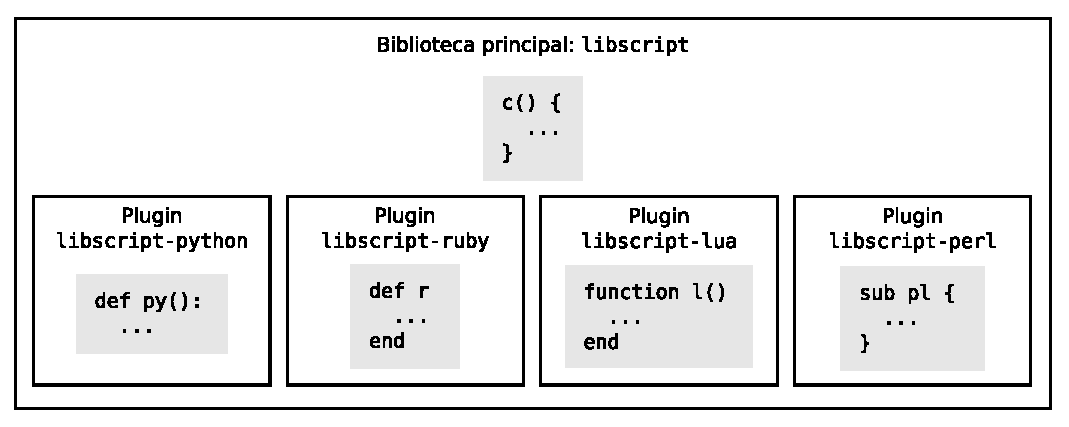
\includegraphics[%
  width=1\columnwidth,
  keepaspectratio]{figura1.eps}\end{center}


\caption{\label{cap:Vis=E3o-geral}Vis�o geral da arquitetura de LibScript}
\end{figure}


LibScript � composta de uma biblioteca din�mica principal, \texttt{libscript},
e \emph{plugins} para diferentes linguagens (Figura~\ref{cap:Vis=E3o-geral}).
A biblioteca principal � ligada a uma aplica��o, e exp�e a ela uma
API de scripting independente de linguagem, que permite executar arquivos,
strings de c�digo e invocar fun��es. Esta biblioteca � uma fina camada
que encaminha estas opera��es para os plugins, que s�o bibliotecas
din�micas auxiliares, carregadas em tempo de execu��o pela biblioteca
principal. Estes plugins embutem os ambientes de execu��o das linguagens
de script.

A aplica��o pode registrar fun��es C na biblioteca principal (ilustrado
pela fun��o \texttt{c\_fun} na figura) e solicitar a ela que execute
scripts que registram fun��es nas diferentes linguagens. Todavia,
a aplica��o n�o interage diretamente com os plugins. Quando a biblioteca
principal recebe c�digo a ser executado em uma determinada linguagem,
ela carrega o plugin adeq�ado (caso este ainda n�o esteja carregado)
e encaminha o c�digo. O plugin ir� executar o script em sua m�quina
virtual, o que pode registrar nela novas fun��es (ilustrado pelas
fun��es \texttt{py\_fun}, \texttt{r\_fun}, \texttt{l\_fun} e \texttt{pl\_fun}
na figura).

A biblioteca principal decide qual plugin carregar atrav�s de um identificador
que especifica qual a linguagem do c�digo a ser executado. Este identificador
pode ser obtido a partir da extens�o de arquivo de um script carregado,
da linha de identifica��o {}``\texttt{\#!}'' no in�cio do script%
\footnote{A linha {}``\texttt{\#!}'' � usada apenas para detectar a linguagem
em que o script � escrito. Por exemplo, uma linha \texttt{\#!/usr/bin/perl
-w} indicar� a carga do plugin \texttt{libscript-perl}, mas o interpretador
Perl em \texttt{/usr/bin} n�o � usado e nem a flag \texttt{-w} passada
� considerada.%
} ou mesmo passado explicitamente pela aplica��o.

%
\begin{figure}
\begin{center}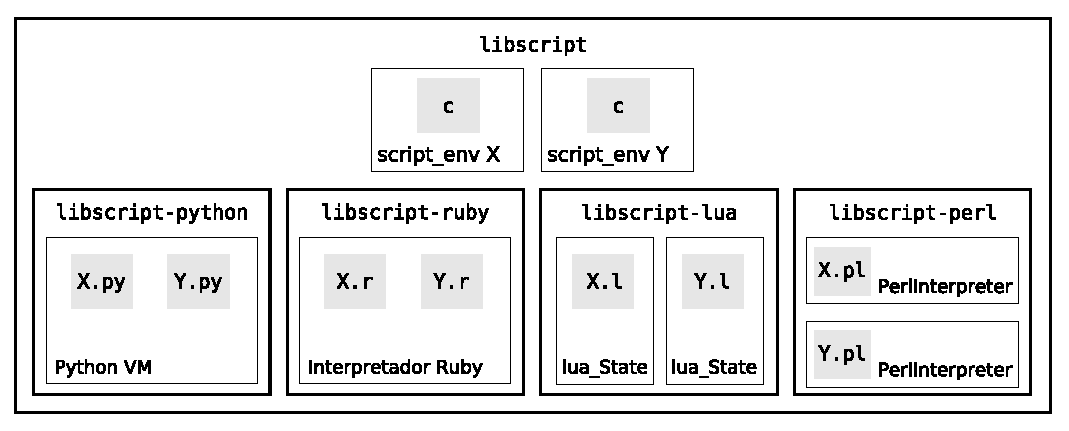
\includegraphics[%
  width=1\columnwidth,
  keepaspectratio]{figura2.eps}\end{center}


\caption{\label{cap:Ambientes-virtuais}Ambientes virtuais em LibScript}
\end{figure}


Fun��es s�o registradas em LibScript em um \emph{ambiente virtual}.
A aplica��o pode criar um ou mais ambientes na biblioteca principal,
identificando-os com um nome. Um ambiente virtual ganha em cada plugin
uma estrutura de dados espec�fica da linguagem (classe, m�dulo, etc.)
que o representar�. No exemplo da Figura~\ref{cap:Ambientes-virtuais}
temos dois ambientes virtuais criados pela aplica��o na biblioteca
principal, \texttt{X} e \texttt{Y}. Em cada um destes ambientes, a
aplica��o registrou uma fun��o C com o nome \texttt{c\_fun} (que podem
ou n�o corresponder � mesma fun��o C). Scripts foram executados nestes
ambientes, o que causou a carga dos plugins. No exemplo, estes scripts
registraram algumas fun��es (\texttt{X.py\_fn}, \texttt{Y.py\_fn},
\texttt{X\#r\_fun}, etc.).

� parte da fun��o para cria��o de ambientes virtuais, todas as demais
fun��es da API de LibScript recebem como par�metro um ambiente virtual
sobre a qual elas devem operar. Isto indica em qual estrutura de C
devem ser armazenadas mensagens de erro e valores de retorno. No caso
de linguagens que permitem m�ltiplos estados de execu��o independentes,
como Lua e Perl, isto indica tamb�m em qual estado o script deve executar.

Quando um script declara uma fun��o no ambiente virtual, esta fun��o
passa a ser acess�vel atrav�s da API de LibScript. Por exemplo, no
plugin Lua, o ambiente virtual � representado por uma tabela com o
nome do ambiente; uma vez que um m�todo Ruby~\texttt{r} � declarado
na classe \texttt{X}, esta fun��o passa a poder ser invocada por C
(atrav�s da API de LibScript) ou pelos outros plugins. Assim, por
exemplo, embora na tabela Lua que implementa o ambiente virtual \texttt{X}
s� conste a fun��o \texttt{l\_fun}, scripts Lua podem invocar as demais
fun��es atrav�s do ambiente virtual, como \texttt{X.c\_fun} e \texttt{X.r\_fun}.
Estas chamadas ser�o tratadas pela biblioteca principal e resolvidas
por ela, no caso de fun��es C como \texttt{X.c\_fun}, ou repassadas
para o plugin apropriado, como no caso de \texttt{X.r\_fun}, realizando
a chamada no plugin Ruby e passando os valores de retorno para o plugin
Lua. A biblioteca principal localiza a fun��o a ser executada consultando
os plugins, conforme ser� explicado na Se��o~\ref{sub:A-API-de-plugins}.

Na implementa��o dos plugins, utilizamos recursos oferecidos pelas
linguagens para tratar acessos a elementos inexistentes nas estruturas,
capturando estes acessos e repassando-os para a biblioteca principal.
Estes recursos ser�o discutidos na Se��o~\ref{sub:Resolu=E7=E3o-de-fun=E7=F5es}.


\subsection{\label{sec:A-Camada-Independente}A API da biblioteca principal}

A API oferecida por LibScript isola a aplica��o das diferentes APIs
oferecidas pelas linguagens de script. N�o se trata apenas de adicionar
uma camada de indire��o entre as chamadas, o que seria apropriado
apenas para os recursos que s�o comuns a todas elas, como inicializa��o
e chamadas de fun��o. A quest�o principal a� s�o os v�rios recursos
particulares a cada linguagem. Uma abordagem pouco pr�tica seria definir
a API como a uni�o dos conjuntos de recursos de todas as linguagens
a ser suportadas (oferecer recursos de manipula��o de seq��ncias para
mapear este recurso de Python, recursos de manipula��o de tabelas
para Lua, e assim por diante). Este caminho traria v�rios problemas:
a API seria complexa e provavelmente precisaria ser estendida a cada
nova linguagem introduzida; mesmo para mapeamentos que aparentemente
poderiam ser reaproveitados (por exemplo, mapear \emph{hashes} de
Python e tabelas de Lua para uma mesma API de \emph{arrays} associativos)
h� o problema de sutis varia��es de sem�ntica entre as implementa��es
dos recursos nas diferentes linguagens. Al�m disso, bindings de aplica��es
poderiam oferecer funcionalidades dispon�veis apenas para uma linguagem,
indo contra a proposta de independ�ncia de linguagem de LibScript.

Outra abordagem �, ao inv�s de expor a API da linguagem � aplica��o,
expor apenas uma API de fun��es da aplica��o para a linguagem e manter
as estruturas de dados e recursos desta restrito ao dom�nio que ser�
invocado. A aplica��o interage com a m�quina virtual enviando strings
de c�digo a ser executado e obt�m resultados de volta quando o script
passa par�metros ao chamar fun��es da aplica��o. Esta abordagem �
proposta em~\cite{thomas02ltn004} e utiliza o que, por exemplo,
Python chama de {}``very high level layer''~\cite{vanrossum06extpy,vanrossum06ref}.
Oferecer uma primitiva para a execu��o de uma string de c�digo � algo
b�sico em linguagens voltadas a script -- \texttt{luaL\_loadstring}
em Lua, \texttt{PyRun\_SimpleString} em Python, \texttt{rb\_eval\_string}
em Ruby , \texttt{perl\_eval\_sv} em Perl~\cite{maceachern06perlembed}.

%
\begin{figure}
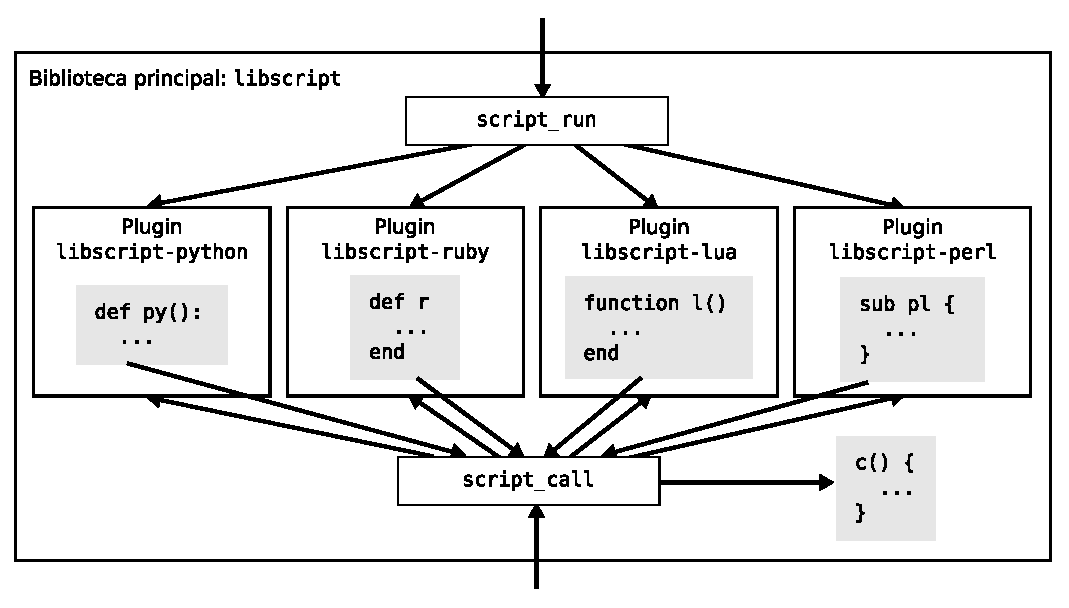
\includegraphics[%
  width=1\columnwidth,
  keepaspectratio]{figura3.eps}


\caption{\label{fig:API-para-execu=E7=E3o}API para execu��o de c�digo em
LibScript}
\end{figure}


LibScript adota esta abordagem mais minimalista para sua API: n�o
s�o oferecidas opera��es espec�ficas para manipula��o de estruturas
de dados, apenas para a \emph{execu��o de strings} -- \texttt{script\_run}
(e a fun��o de conveni�ncia \texttt{script\_run\_file}, que l� um
arquivo e o envia para \texttt{script\_run}) -- e \emph{chamadas de
fun��o} com tipos b�sicos (n�meros e strings) -- \texttt{script\_call}.
Opera��es sobre dados mais complexos de tipos espec�ficos de cada
linguagem, quando necess�rias, podem ser encapsuladas em fun��es implementadas
nas linguagens de script. Pode-se ainda referenciar objetos da linguagem
a partir de C armazenando-as em estruturas na linguagem de script
e retornando a C �ndices num�ricos destas estruturas, servindo como
\emph{handles} de alto n�vel para os objetos.

A Figura~\ref{fig:API-para-execu=E7=E3o} ilustra a intera��o entre
a aplica��o, a biblioteca principal e os plugins em rela��o a estas
duas opera��es fundamentais, simbolizadas pelas fun��es \texttt{script\_run}
e \texttt{script\_call}. Para a execu��o de strings, a biblioteca
principal recebe da aplica��o a entrada e repassa o c�digo a ser executado
para o plugin apropriado. Em \texttt{script\_run}, s�o passadas duas
strings, uma identificando a linguagem e outra contendo o c�digo;
em \texttt{script\_run\_file}, um nome de arquivo%
\footnote{Para c�digo executado com \texttt{script\_run\_file}, a linguagem
� automaticamente detectada como discutido na se��o anterior.%
}. O exemplo a seguir declara um ambiente virtual, registra uma fun��o
C chamada \texttt{hello} e a invoca a partir de c�digo Lua:

\begin{lyxcode}
{\footnotesize script\_env{*}~env~=~script\_init(\char`\"{}exemplo\char`\"{});}{\footnotesize \par}

{\footnotesize script\_new\_function(env,~hello,~\char`\"{}hello\char`\"{});}{\footnotesize \par}

{\footnotesize script\_run(env,~\char`\"{}lua\char`\"{},~\char`\"{}exemplo.hello()\char`\"{});}{\footnotesize \par}
\end{lyxcode}


O ambiente virtual � declarado com a fun��o \texttt{script\_init},
que recebe o nome que identificar� o ambiente e retorna um identificador
do tipo \texttt{script\_env}, um ponteiro opaco que representa um
ambiente virtual. A fun��o C � registrada usando a fun��o \texttt{script\_new\_\-function},
que recebe como par�metros o ambiente, a fun��o a ser registrada e
o nome que a fun��o ter� no ambiente virtual. No c�digo Lua, a fun��o
� acessada como um elemento \texttt{hello} (nome registrado da fun��o)
da tabela global \texttt{exemplo} (nome do ambiente virtual).

Para a chamada de fun��es, a aplica��o deve passar os par�metros de
entrada (a forma ser� discutida mais adiante), e chamar \texttt{script\_call},
indicando o nome de uma fun��o registrada no ambiente virtual. A mesma
fun��o \texttt{script\_call} � usada pelos plugins quando eles desejam
invocar fun��es do ambiente virtual registradas em C ou implementadas
por outros plugins.

Por este motivo, procuramos usar uma API para transfer�ncia de dados
gen�rica, a ser usada tanto na entrada como na sa�da de dados, tanto
na comunica��o entre a aplica��o e a biblioteca principal como entre
a biblioteca principal e os plugins. Optamos por uma abordagem similar
�s empregadas em Lua (Se��o~\ref{sub:Lua-chamada}) e Perl (Se��o~\ref{sub:Perl-call})
para o envio de dados na passagem de par�metros e obten��o de valores
de retorno, usando um buffer interno como �rea de transfer�ncia. Diferentemente
destas linguagens, entretanto, passamos �ndices para os par�metros
explicitamente ao inv�s de empregar uma disciplina de pilha. As fun��es
\texttt{script\_}\{\texttt{get},\texttt{put}\}\_\{\texttt{string},\texttt{int},\texttt{double},\texttt{bool}\}
s�o usadas na entrada e sa�da de valores. As fun��es \texttt{script\_put\_}{*}
armazenam valores no buffer interno e \texttt{script\_get\_}{*} os
removem. Uma chamada a uma fun��o \texttt{teste} passando uma string
e um inteiro como par�metros e obtendo um inteiro como resultado �
realizada da seguinte forma:

\begin{lyxcode}
{\footnotesize script\_put\_string(env,~0,~\char`\"{}entrada\char`\"{});}~\emph{\footnotesize /{*}~�ndice~0:~\char`\"{}entrada\char`\"{}~{*}/}{\footnotesize \par}

{\footnotesize script\_put\_int(env,~1,~2);~~~~~~~~~~~}~\emph{\footnotesize /{*}~�ndice~1:~2~{*}/}{\footnotesize \par}

{\footnotesize script\_call(env,~\char`\"{}teste\char`\"{});}{\footnotesize \par}

{\footnotesize resultado~=~script\_get\_int(env,~0);~~}~\emph{\footnotesize /{*}~retorna~�ndice~0~{*}/}{\footnotesize \par}
\end{lyxcode}


Chamadas de fun��o s�o disponibilizadas como uma opera��o primitiva
pois elas permitem um grau m�nimo de interoperabilidade de forma independente
de linguagem. Dois objetivos s�o atingidos desta forma. O primeiro
� que assim programas C embutindo LibScript podem acessar a funcionalidade
de scripts carregados sem precisar incluir no seu c�digo strings de
texto em alguma linguagem espec�fica, por exemplo, inserindo em seu
c�digo uma chamada a uma fun��o de \emph{callback} a ser definida
via script. Note que no exemplo acima, n�o � especificada a linguagem
em que a fun��o \texttt{teste} � implementada. Se a chamada fosse
feita via execu��o de string de c�digo, isto atrelaria a aplica��o
a pelo menos uma linguagem de script. Usando \texttt{script\_run\_file}
e \texttt{script\_call}, pode-se implementar uma aplica��o extens�vel
sem especificar explicitamente a linguagem de script a ser usada.
O segundo objetivo � permitir que os pr�prios plugins possam invocar
fun��es definidas em outros plugins. De qualquer forma, necessariamente
ter�amos que prover aos plugins uma fun��o de chamada, para que eles
pudessem invocar as fun��es C registradas em LibScript. Tornar a fun��o
de chamada gen�rica o suficiente para que possa invocar tamb�m fun��es
implementadas nos pr�prios plugins n�o torna, ent�o, a API da biblioteca
principal mais complexa.

O buffer de LibScript foi projetado para ser usado apenas como uma
�rea de transfer�ncia tempor�ria entre a biblioteca principal e os
plugins, e n�o como uma facilidade geral para armazenamento e manipula��o
de dados. Assim, a sua API � voltada para a inser��o e remo��o seq�encial
de elementos. Por exemplo, a inser��o de um elemento na posi��o 0
automaticamente zera o buffer, evitando em muitos casos a necessidade
de usar a fun��o \texttt{script\_reset\_buffer}, que realiza tal opera��o
explicitamente.

Fun��es C registradas com \texttt{script\_new\_function} devem receber
o ambiente virtual como par�metro e retornar um c�digo de erro. As
fun��es \texttt{script\_get\_}{*} e \texttt{script\_put\_}{*} s�o
usadas para receber par�metros e retornar valores ao implementar fun��es
que podem ser chamadas via LibScript, da mesma forma que s�o usadas
para passar par�metros e obter valores de retorno ao realizar chamadas
com \texttt{script\_call}.

\begin{lyxcode}
{\footnotesize script\_err~teste\_lua(script\_env{*}~env)~\{}{\footnotesize \par}

~\emph{\footnotesize ~~/{*}~Entrada,~�ndice~0:~string~{*}/}{\footnotesize \par}

~{\footnotesize ~~char{*}~entrada~=~script\_get\_string(env,~0);}{\footnotesize \par}

~\emph{\footnotesize ~~/{*}~Entrada,~�ndice~1:~inteiro~{*}/}{\footnotesize \par}

~{\footnotesize ~~int~n~=~script\_get\_int(env,~1);}{\footnotesize \par}

~\emph{\footnotesize ~~/{*}~Sai~da~fun��o~com~erro~se~algum~script\_get\_{*}~falhou~{*}/}{\footnotesize \par}

~{\footnotesize ~~SCRIPT\_CHECK\_INPUTS(env);}{\footnotesize \par}

~{\footnotesize ~~printf(\char`\"{}Recebi~\%s~e~\%ld~\textbackslash{}n\char`\"{},~entrada,~n);}{\footnotesize \par}

~{\footnotesize ~~free(entrada);}{\footnotesize \par}

~\emph{\footnotesize ~~/{*}~Retorno,~�ndice~0:~inteiro~{*}/}{\footnotesize \par}

~{\footnotesize ~~script\_put\_int(env,~0,~42);}{\footnotesize \par}

~{\footnotesize ~~return~SCRIPT\_OK;}{\footnotesize \par}

{\footnotesize \}}{\footnotesize \par}
\end{lyxcode}


Em LibScript as strings retornadas por \texttt{script\_get\_string}
pertencem � fun��o chamadora, sendo responsabilidade dela desalocar
a mem�ria, diferentemente do que ocorre nas fun��es similares das
APIs das linguagens discutidas neste trabalho. Tal decis�o foi tomada
devido ao car�ter tempor�rio do buffer de LibScript: retornar ao chamador
um ponteiro para uma string cuja validade seria restrita at� a pr�xima
chamada da API seria algo pouco intuitivo, e na pr�tica for�aria freq�entemente
o programador a fazer uma c�pia da string.


\subsection{A API de plugins\label{sub:A-API-de-plugins}}

Um plugin que embute uma linguagem de script deve implementar quatro
opera��es: \texttt{init}, \texttt{run}, \texttt{call} e \texttt{done}.
A biblioteca principal espera que a biblioteca din�mica que implementa
o plugin de uma linguagem exporte quatro fun��es, com nomes do tipo
\texttt{script\_plugin\_}\emph{{[}opera��o{]}}\texttt{\_}\emph{{[}linguagem{]}}.

A fun��o \texttt{script\_plugin\_init\_}\emph{{[}linguagem{]}} � respons�vel
pela inicializa��o de um plugin, e � chamada pela fun��o \texttt{script\_init}
da biblioteca principal. Na inicializa��o de um plugin, a biblioteca
principal passa � fun��o \texttt{script\_plugin\_init\_}\emph{{[}linguagem{]}}
um ponteiro \texttt{script\_env} e recebe um \texttt{script\_plugin\_state},
que � um tipo opaco que � sempre passado de volta ao plugin nas demais
chamadas. Cada plugin define a sua representa��o interna para \texttt{script\_plugin\_state}.
Tipicamente, o estado da m�quina virtual e o ponteiro para o ambiente
LibScript devem ser armazenados de modo a ser posteriormente acess�veis
a partir deste handle. Na Se��o~\ref{sub:Representa=E7=E3o-de-estados}
discutiremos como cada plugin representa o ambiente e o seu estado
interno em \texttt{script\_plugin\_state}.

A fun��o \texttt{script\_plugin\_run\_}\emph{{[}linguagem{]}} � invocada
por \texttt{script\_run}. Ela recebe uma string contendo c�digo da
linguagem de script, executa este c�digo na m�quina virtual e retorna
um valor de status indicando sucesso ou a ocorr�ncia de erros de compila��o
ou execu��o. No caso de erros, os plugins devem capturar exce��es
disparadas pela m�quina virtual e retornar a constante \texttt{SCRIPT\_ERRLANGRUN}.
Caso seja poss�vel obter da linguagem uma mensagem de erro, esta pode
ser propagada usando a fun��o \texttt{script\_set\_error\_message}
da biblioteca principal. A mensagem armazenada por ela poder� ser
posteriormente consultada pela aplica��o com a fun��o \texttt{script\_error\_message}.

A fun��o \texttt{script\_plugin\_call\_}\emph{{[}linguagem{]}} � usada
por \texttt{script\_call}, e � respons�vel por realizar chamadas a
fun��es implementadas na linguagem embutida pelo plugin. Se a fun��o
foi definida no plugin, isto �, se uma fun��o com o nome solicitado
foi registrada na estrutura de dados que descreve o ambiente na m�quina
virtual, ela ser� executada, e o sucesso ou falha da execu��o ser�
reportado de forma igual a \texttt{script\_plugin\_run\_}\emph{{[}linguagem{]}}.
Caso a fun��o solicitada n�o tenha sido definida na m�quina virtual,
\texttt{script\_plugin\_call\_}\emph{\-{[}linguagem{]}} deve retornar
a constante \texttt{SCRIPT\_ERRFNUNDEF}. Par�metros de entrada e valores
de retorno s�o passados atrav�s do buffer de par�metros, usando as
mesmas fun��es \texttt{script\_get\_{*}} e \texttt{script\_put\_{*}}
da biblioteca principal que s�o usadas para a passagem de dados entre
a aplica��o e a biblioteca principal.

A implementa��o da fun��o \texttt{script\_call} na biblioteca principal
faz uso deste comportamento dos plugins para invocar fun��es de modo
independente de linguagem. Inicialmente, ela tenta encontrar uma fun��o
solicitada na lista de fun��es C registradas. Caso n�o haja uma fun��o
C no ambiente virtual com este nome, \texttt{script\_call} tenta localizar
a fun��o nos plugins carregados, chamando a fun��o com \texttt{script\_plugin\_call\_}\emph{{[}linguagem{]}}
em cada plugin, e tentando o pr�ximo a cada vez que recebe \texttt{SCRIPT\_ERRFNUNDEF}.

Finalmente, a fun��o \texttt{script\_plugin\_done\_}\emph{{[}linguagem{]}}
� chamada por \texttt{script\_done} quando um ambiente virtual � encerrado.
Dependendo da representa��o interna usada no plugin, a finaliza��o
de um estado pode ou n�o implicar na finaliza��o da m�quina virtual.
Preferencialmente, esta fun��o deve remover a estrutura que descreve
o ambiente virtual, mas, como veremos na Se��o~\ref{sub:Encerramento-de-estados},
isto nem sempre � poss�vel.


\section{Implementa��o dos plugins\label{sec:Implementa=E7=E3o-dos-plugins}}

Nesta se��o discutiremos os principais aspectos envolvidos na implementa��o
dos plugins desenvolvidos neste estudo de caso. Implementamos plugins
para as linguagens Python, Ruby, Lua e Perl. Apresentaremos aqui como
� feita a representa��o dos estados virtuais em cada plugin (Se��o~\ref{sub:Representa=E7=E3o-de-estados}),
quest�es envolvendo o encerramento de estados (Se��o~\ref{sub:Encerramento-de-estados}),
passagem de par�metros entre a biblioteca principal e os plugins (Se��o~\ref{sub:Passagem-de-par=E2metros}),
como a chamada de fun��es a partir de scripts � tratada pelos plugins
(Se��o~\ref{sub:Resolu=E7=E3o-de-fun=E7=F5es}) e a captura de erros
(Se��o~\ref{sub:Captura-de-erros}).


\subsection{Representa��o de estados\label{sub:Representa=E7=E3o-de-estados}}

O design de LibScript permite que plugins mantenham m�ltiplos estados
de execu��o independentes. Idealmente estes estados seriam totalmente
isolados entre si, como por exemplo diferentes inst�ncias da m�quina
virtual, oferecendo maior seguran�a ao ambiente de execu��o dos scripts.
Todavia, as linguagens oferecem diferentes graus de isolamento poss�vel
entre estados independentes. Lua e Perl permitem m�ltiplas inst�ncias
isoladas do ambiente de execu��o de forma simples, uma vez que as
chamadas � API incluem um identificador de estado%
\footnote{O recurso de m�ltiplos estados independentes � opcional em Perl, selecionado
durante a compila��o da biblioteca do interpretador.%
}. J� linguagens que mant�m estado de forma est�tica, como Python e
Ruby, n�o permitem trabalhar com m�ltiplos estados isolados facilmente%
\footnote{O modelo de threads de Python oferece uma forma de alternar entre
estados na m�quina virtual obtendo objetos \texttt{PyThreadState}
atrav�s da chamada \texttt{Py\_NewInterpreter}, mas isto pode causar
problemas quando m�dulos de extens�o escritos em C utilizam vari�veis
globais est�ticas ou quando m�dulos manipulam o seu pr�prio dicion�rio,
que � compartilhado entre estados. A documenta��o diz, desde 1999,
que {}``\emph{This is a hard-to-fix bug that will be addressed in
a future release.}''~\cite{vanrossum99api,vanrossum06api}%
}. Nas linguagens que n�o permitem m�ltiplas inst�ncias da m�quina
virtual, podemos definir apenas espa�os de nomes separados para os
ambientes virtuais LibScript, que compartilham um �nico estado global
de execu��o dentro do plugin. � representa��o de um estado de execu��o
relativo a um ambiente virtual LibScript dentro de um plugin damos
o nome de \emph{estado virtual}, que pode ou n�o corresponder a um
estado de execu��o isolado.

Como comentado na se��o anterior, a fun��o \texttt{script\_plugin\_init\_}\emph{lin\-gua\-gem}
retorna � biblioteca principal um \texttt{script\_plugin\_state},
que � a representa��o opaca do seu estado virtual. O conte�do desta
representa��o varia de linguagem para linguagem, mas o princ�pio b�sico
� que dois dados devem estar dispon�veis a partir deste valor: uma
refer�ncia para o ambiente virtual LibScript, recebido como par�metro
para \texttt{script\_plugin\_init\_}\emph{lin\-gua\-gem}, para que
o plugin possa fazer chamadas � biblioteca principal, e um identificador
que permita ao plugin acessar a estrutura de dados que representa
na linguagem o espa�o de nome de fun��es acess�veis via LibScript.
No plugin Lua, esta estrutura � uma tabela; em Python, um m�dulo;
em Ruby, uma classe; e em Perl, um pacote.

Em LibScript-Lua, estados s�o implementados como \texttt{lua\_State}s
(Se��o~\ref{sub:Lua-Registro}). Desta forma, scripts executados
em um ambiente s�o plenamente isolados dos demais ambientes. Por exemplo,
a altera��o do valor de uma vari�vel global em um ambiente n�o afeta
os demais. De fato, o \texttt{script\_plugin\_state} retornado pelo
plugin Lua � simplesmente o \texttt{lua\_State} convertido via cast.
O ponteiro para o ambiente LibScript � armazenado em Lua no registro,
da seguinte forma:

\begin{lyxcode}
\emph{\footnotesize /{*}~Empilha~o~�ndice~{*}/}{\footnotesize \par}

{\footnotesize lua\_pushstring(L,~\char`\"{}LibScript.env\char`\"{});}{\footnotesize \par}

\emph{\footnotesize /{*}~Empilha~o~ambiente~LibScript~{*}/}{\footnotesize \par}

{\footnotesize lua\_pushlightuserdata(L,~env);}{\footnotesize \par}

\emph{\footnotesize /{*}~registro{[}\char`\"{}LibScript.env\char`\"{}{]}~=~env~{*}/}{\footnotesize \par}

{\footnotesize lua\_settable(L,~LUA\_REGISTRYINDEX);}{\footnotesize \par}
\end{lyxcode}


O plugin cria neste \texttt{lua\_State} uma tabela que representar�
o ambiente virtual para scripts Lua. Esta tabela � armazenada no \texttt{lua\_State}
como uma vari�vel global com o nome do ambiente virtual.

Em LibScript-Perl os estados s�o isolados como em Lua. Cada estado
criado inicializa uma nova inst�ncia de \texttt{PerlInterpreter}.
Neste interpretador, � criado um pacote que ser� a representa��o do
ambiente vis�vel a partir de c�digo Perl. O tipo \texttt{script\_plugin\_state},
ent�o, � um \emph{typedef} para \texttt{PerlInterpreter}{*}.

Como discutido na Se��o~\ref{sub:Perl-registro}, a implementa��o
de fun��es C exportadas para um interpretador Perl � feita escrevendo
um m�dulo de extens�o usando o pr�-processador XS, e a forma de obter
comunica��o no sentido Perl$\rightarrow$C em uma m�quina virtual
embutida � ligando um m�dulo de extens�o juntamente com a m�quina
virtual. Assim, parte do plugin LibScript-Perl � implementado como
um m�dulo XS, exposto na m�quina virtual embutida como o pacote Perl
\texttt{LibScript}. Durante a inicializa��o de um estado virtual,
o ponteiro para o ambiente virtual LibScript � armazenado neste pacote,
na vari�vel \texttt{\$LibScript::env}. O pacote que representa o ambiente
virtual � criado pela fun��o \texttt{script\_plugin\_init\_perl},
executando a string de c�digo \texttt{\char`\"{}package} \emph{{[}ambiente{]}}\texttt{;\char`\"{}}
com a fun��o \texttt{Perl\_eval\_pv}.

Como Python n�o disp�e de facilidades para disparar m�ltiplas m�quinas
virtuais plenamente isoladas, o plugin Python implementa estados virtuais
apenas como m�dulos separados, compartilhando um mesmo estado global.
Durante a inicializa��o de um estado, � criado um m�dulo Python com
o nome do ambiente. O seguinte trecho da fun��o \texttt{script\_plugin\_init\_python}
exibe a seq��ncia onde o m�dulo � criado e importado:

\begin{lyxcode}
\emph{\footnotesize /{*}~Obt�m~o~nome~do~ambiente~{*}/}{\footnotesize \par}

{\footnotesize char{*}~namespace~=~script\_namespace(env);}{\footnotesize \par}

\emph{\footnotesize /{*}~Cria~o~m�dulo.~O~primeiro~par�metro~�~o~nome~do~m�dulo,~o~segundo}{\footnotesize \par}

~\emph{\footnotesize ~~a~lista~de~m�todos~do~m�dulo,~que~ser�~inicialmente~vazio.~{*}/}{\footnotesize \par}

{\footnotesize PyObject{*}~module~=~Py\_InitModule3(namespace,~NULL);}{\footnotesize \par}

\emph{\footnotesize /{*}~Obt�m~dicion�rio~de~globais~{*}/}{\footnotesize \par}

{\footnotesize PyObject{*}~globals~=~PyModule\_GetDict(PyImport\_AddModule(\char`\"{}\_\_builtin\_\_\char`\"{}));}{\footnotesize \par}

\emph{\footnotesize /{*}~Atribui~o~m�dulo~�~vari�vel~global~com~o~seu~nome.~{*}/}{\footnotesize \par}

{\footnotesize PyDict\_SetItemString(globals,~namespace,~module);}{\footnotesize \par}
\end{lyxcode}


O tipo \texttt{script\_plugin\_state} � um \emph{typedef} para \texttt{PyObject{*}}.
O objeto retornado pela fun��o de inicializa��o � o dicion�rio de
elementos do m�dulo, obtido com \texttt{PyModule\_GetDict\-(module)}.
Neste dicion�rio, armazenamos o ponteiro do ambiente virtual como
o atributo privado \texttt{\_\_env}.

De forma similar, em Ruby estados virtuais s�o implementados como
classes que compartilham um mesmo estado global, j� que Ruby tamb�m
n�o permite m�ltiplos ambientes de execu��o isolados. Na fun��o de
inicializa��o \texttt{script\_plugin\_init\_ruby}, uma classe com
o nome do ambiente virtual � criada usando a fun��o \texttt{rb\_define\_class}.
O ponteiro do ambiente virtual � armazenado em uma constante da classe
como um n�mero. O \texttt{VALUE} referente � classe � retornado como
o \texttt{script\_plugin\_state}.

\begin{lyxcode}
{\footnotesize VALUE~state;}{\footnotesize \par}

\emph{\footnotesize /{*}~...~(inicializa��o~do~interpretador~omitida)~...~{*}/}{\footnotesize \par}

\emph{\footnotesize /{*}~class\_name~�~o~nome~do~ambiente~virtual,}{\footnotesize \par}

~\emph{\footnotesize ~~com~a~inicial~convertida~para~mai�sculas,}{\footnotesize \par}

~\emph{\footnotesize ~~respeitando~a~conven��o~de~nomes~de~classe~Ruby~{*}/}{\footnotesize \par}

{\footnotesize state~=~rb\_define\_class(class\_name,~rb\_cObject);}{\footnotesize \par}

\emph{\footnotesize /{*}~Isto~assume~que~void{*}~cabe~em~um~long~{*}/}{\footnotesize \par}

{\footnotesize rb\_const\_set(state,~rb\_intern(\char`\"{}@@LibScriptEnv\char`\"{}),~INT2NUM((long)env));~~~~}{\footnotesize \par}

\emph{\footnotesize /{*}~...~{*}/}{\footnotesize \par}

{\footnotesize return~(script\_plugin\_state)~state;}{\footnotesize \par}
\end{lyxcode}

\subsection{Encerramento de estados\label{sub:Encerramento-de-estados}}

Como Lua e Perl representam estados de forma independente, o encerramento
de um estado nestes plugins � simples: a estrutura da linguagem que
encapsula o ambiente completo de execu��o � encerrada. A implementa��o
da fun��o de finaliza��o no plugin Lua � a seguinte:

\begin{lyxcode}
{\footnotesize void~script\_plugin\_done\_lua(script\_plugin\_state~state)~\{}{\footnotesize \par}

~{\footnotesize ~}~\emph{\footnotesize /{*}~Em~Lua,~um~state~�~um~lua\_State~{*}/}{\footnotesize \par}

~{\footnotesize ~~lua\_State{*}~L~=~(lua\_State{*})~state;}{\footnotesize \par}

~{\footnotesize ~}~\emph{\footnotesize /{*}~Encerra~o~estado.~N�o~afeta~outros~ambientes.~{*}/}{\footnotesize \par}

~{\footnotesize ~~lua\_close(L);}{\footnotesize \par}

{\footnotesize \}}{\footnotesize \par}
\end{lyxcode}


Em Perl, o processo, embora um tanto mais elaborado, � essencialmente
similar:

\begin{lyxcode}
{\footnotesize void~script\_plugin\_done\_perl(script\_perl\_state{*}~state)~\{}{\footnotesize \par}

~{\footnotesize ~}~\emph{\footnotesize /{*}~Algumas~macros~assumem~que~o~ponteiro~do~interpretador}{\footnotesize \par}

~\emph{\footnotesize ~~~~~se~chama~my\_perl.~{*}/}{\footnotesize \par}

~{\footnotesize ~~PerlInterpreter{*}~my\_perl~=~(PerlInterpreter{*})~state;}{\footnotesize \par}

~{\footnotesize ~}~\emph{\footnotesize /{*}~Algumas~opera��es~atuam~sobre~o~{}``estado~atual'',}{\footnotesize \par}

~\emph{\footnotesize ~~~~~ent�o~a~macro~PERL\_SET\_CONTEXT~deve~ser~usada~para}{\footnotesize \par}

~\emph{\footnotesize ~~~~~alternar~o~interpretador~ativo~{*}/}{\footnotesize \par}

~{\footnotesize ~~PERL\_SET\_CONTEXT(my\_perl);}{\footnotesize \par}

~\emph{\footnotesize ~~/{*}~Esta~flag~deve~ser~ativada~para~que~a~limpeza~do}{\footnotesize \par}

~\emph{\footnotesize ~~~~~ambiente~seja~completa,~o~que~�~necess�rio~quando}{\footnotesize \par}

~\emph{\footnotesize ~~~~~pode~haver~mais~de~um~interpretador~ativo~{*}/}{\footnotesize \par}

~{\footnotesize ~~PL\_perl\_destruct\_level~=~1;}{\footnotesize \par}

~\emph{\footnotesize ~~/{*}~Encerramento~do~interpretador~{*}/}{\footnotesize \par}

~{\footnotesize ~~perl\_destruct(my\_perl);}{\footnotesize \par}

~{\footnotesize ~~perl\_free(my\_perl);}{\footnotesize \par}

{\footnotesize \}}{\footnotesize \par}
\end{lyxcode}


Em Python e Ruby, o plugin precisa manter o controle do n�mero de
estados ativos para desalocar a m�quina virtual somente quando este
chegar a zero. Al�m disso, tanto em Ruby como em Python n�o h� recursos
nas APIs (ou nas linguagens, de fato) para remover, respectivamente,
classes ou m�dulos. Em Ruby, poder�amos atribuir \texttt{nil} � constante
que representa a classe que descreve o ambiente virtual, mas depois
disso n�o � poss�vel definir uma nova classe em seu lugar: tanto \texttt{rb\_define\_class}
via C como \texttt{class} \emph{{[}Nome{]}} via Ruby geram um erro
indicando que o valor j� foi definido com outro tipo. Como Ruby possui
classes abertas, uma constru��o \texttt{class} \emph{{[}Nome{]}} para
um \emph{{[}Nome{]}} j� existente � entendida como a continua��o da
descri��o da classe, e n�o como a redefini��o de \emph{{[}Nome{]}}.
Python, por sua vez, n�o disponibiliza recursos na API para a descarga
de m�dulos, mas permite atribuir \texttt{None} � global referente
ao m�dulo. O m�dulo pode ser importado novamente, mas a mesma inst�ncia
dele, armazenada internamente por Python, ser� retornada. A seguinte
sess�o interativa de linha de comando permite observar este comportamento,
que ocorre tanto diretamente em Python como via a API de C:

\begin{lyxcode}
{\footnotesize >\,{}>\,{}>~import~sys}{\footnotesize \par}

{\footnotesize >\,{}>\,{}>~sys.foo~=~\char`\"{}hello\char`\"{}}{\footnotesize \par}

{\footnotesize >\,{}>\,{}>~sys.foo}{\footnotesize \par}

{\footnotesize 'hello'}{\footnotesize \par}

{\footnotesize >\,{}>\,{}>~sys~=~None}{\footnotesize \par}

{\footnotesize >\,{}>\,{}>~import~sys}{\footnotesize \par}

{\footnotesize >\,{}>\,{}>~sys.foo}{\footnotesize \par}

{\footnotesize 'hello'~}{\footnotesize \par}
\end{lyxcode}


Assim, as estruturas de dados referentes aos estados LibScript n�o
s�o encerrados nos plugins Python e Ruby. Esta � a implementa��o da
rotina de encerramento no plugin Ruby:

\begin{lyxcode}
{\footnotesize void~script\_plugin\_done\_ruby(script\_ruby\_state~state)~\{}{\footnotesize \par}

~\emph{\footnotesize ~~/{*}~Decrementa~o~contador~de~estados,}{\footnotesize \par}

~\emph{\footnotesize ~~~~~uma~vari�vel~global}~{\footnotesize static}~\emph{\footnotesize do~plugin.~{*}/}{\footnotesize \par}

~{\footnotesize ~~script\_ruby\_state\_count-{}-;}{\footnotesize \par}

~\emph{\footnotesize ~~/{*}~Finaliza~o~interpretador~se~este~for~o~�ltimo~estado.~{*}/}{\footnotesize \par}

~{\footnotesize ~~if~(script\_ruby\_state\_count~==~0)}{\footnotesize \par}

~{\footnotesize ~~~~~ruby\_finalize();}{\footnotesize \par}

{\footnotesize \}}{\footnotesize \par}
\end{lyxcode}
A implementa��o no plugin Python � basicamente igual:

\begin{lyxcode}
{\footnotesize void~script\_plugin\_done\_python(script\_python\_state~state)~\{}{\footnotesize \par}

~{\footnotesize ~~script\_python\_state\_count-{}-;}{\footnotesize \par}

~{\footnotesize ~~if~(script\_python\_state\_count~==~0)}{\footnotesize \par}

~{\footnotesize ~~~~~Py\_Finalize();}{\footnotesize \par}

{\footnotesize \}}{\footnotesize \par}
\end{lyxcode}

\subsection{Passagem de par�metros\label{sub:Passagem-de-par=E2metros}}

A transfer�ncia de dados entre a biblioteca principal e os plugins
� concentrada em duas opera��es: uma para passar o conte�do do buffer
de par�metros de LibScript para o espa�o de dados da m�quina virtual
e outra para realizar a opera��o inversa. A primeira � usada na passagem
de par�metros de entrada quando fun��es da linguagem de script s�o
chamadas por C e para a obten��o dos valores de retorno quando a linguagem
de script faz chamadas que s�o tratadas por C. A segunda opera��o,
de forma complementar, � usada para os valores de retorno quando C
chama a linguagem de script e para os par�metros de entrada quando
uma chamada feita pela linguagem de script � tratada por c�digo C.

Na implementa��o do plugin LibScript-Lua, a fun��o \texttt{script\_\-lua\_\-stack\_\-to\_\-buffer}
converte o conte�do da pilha de Lua para o buffer de par�metros de
LibScript. A fun��o do plugin respons�vel por invocar fun��es Lua
a partir de C, \texttt{script\_\-plugin\_\-call\_\-lua}, usa a
fun��o \texttt{script\_\-lua\_\-stack\_\-to\_\-buffer} para armazenar
no buffer LibScript os valores de retorno da fun��o Lua invocada,
j� que estes s�o retornados na pilha virtual. Quando o c�digo Lua
chama fun��es implementadas em C ou em outro plugin, \texttt{script\_\-lua\_\-stack\_\-to\_\-buffer}
� usada para converter os par�metros de entrada da fun��o, tamb�m
recebidos na pilha virtual. A seguir, vemos a implementa��o desta
fun��o:

\begin{lyxcode}
{\footnotesize static~void~script\_lua\_stack\_to\_buffer(script\_env{*}~env,~lua\_State~{*}L)~\{}{\footnotesize \par}

~{\footnotesize ~~int~nargs;~int~i;~}{\footnotesize \par}

~{\footnotesize ~}~\emph{\footnotesize /{*}~N�mero~de~elementos~na~pilha~de~Lua~{*}/}{\footnotesize \par}

~{\footnotesize ~~nargs~=~lua\_gettop(L);}{\footnotesize \par}

~{\footnotesize ~~script\_reset\_buffer(env);}~\emph{\footnotesize /{*}~Esvazia~o~buffer~LibScript~{*}/}{\footnotesize \par}

~{\footnotesize ~~for~(i~=~1;~i~<=~nargs;~i++)~\{}{\footnotesize \par}

~{\footnotesize ~~~~}~\emph{\footnotesize /{*}~Verifica~o~tipo~Lua~do~elemento~na~posi��o~i~da~pilha}{\footnotesize \par}

~\emph{\footnotesize ~~~~~e~para~cada~tipo,~converte~o~elemento~e~o~armazena~no~buffer~{*}/}{\footnotesize \par}

~{\footnotesize ~~~~~switch(lua\_type(L,~i))~\{~}{\footnotesize \par}

~{\footnotesize ~~~~~case~LUA\_TNUMBER:}{\footnotesize \par}

~{\footnotesize ~~~~~~~~script\_put\_double(env,~i-1,~lua\_tonumber(L,~i));~break;~}{\footnotesize \par}

~{\footnotesize ~~~~~case~LUA\_TSTRING:}{\footnotesize \par}

~{\footnotesize ~~~~~~~~script\_put\_string(env,~i-1,~lua\_tostring(L,~i));~break;}{\footnotesize \par}

~{\footnotesize ~~~~~case~LUA\_TBOOLEAN:}{\footnotesize \par}

~{\footnotesize ~~~~~~~~script\_put\_bool(env,~i-1,~lua\_toboolean(L,~i));~break;}{\footnotesize \par}

~{\footnotesize ~~~~~default:}{\footnotesize \par}

~\emph{\footnotesize ~~~~~~~~/{*}~Tipos~n�o~tratados~s�o~substitu�dos~por~zero.~{*}/}{\footnotesize \par}

~{\footnotesize ~~~~~~~~script\_put\_double(env,~i-1,~0);}{\footnotesize \par}

~{\footnotesize ~~~~~\}}{\footnotesize \par}

~{\footnotesize ~~\}}{\footnotesize \par}

{\footnotesize \}}{\footnotesize \par}
\end{lyxcode}


Assumimos em LibScript strings no formato de C: a fun��o \texttt{script\_put\_string}
copia a string passada at� o primeiro \texttt{'\textbackslash{}0'}.
Assim, ao obter strings de linguagens que permitem conte�do arbitr�rio,
estas ser�o truncadas caso contenham \texttt{'\textbackslash{}0'}.
Por isso, no plugin Lua usamos diretamente a fun��o \texttt{lua\_tostring},
e n�o a fun��o mais geral \texttt{lua\_tolstring} (que retorna tamb�m
o tamanho do buffer). Esta decis�o de projeto coincide com o objetivo
explicado anteriormente de restringirmos a API da biblioteca principal
a recursos dispon�veis em todas as linguagens.

Os valores de tipos desconhecidos s�o substitu�dos pelo valor zero,
o que mant�m a posi��o dos demais valores na lista de argumentos.
Optamos por n�o sinalizar erro nesta situa��o para evitar aqui a gera��o
de exce��es, o que complicaria a exposi��o. A captura e propaga��o
de erros ser�o vistas na Se��o~\ref{sub:Captura-de-erros}.

A segunda fun��o de transfer�ncia de dados de LibScript-Lua, \texttt{script\_lua\_buffer\_to\_stack},
obt�m os valores do buffer LibScript e os insere na pilha virtual
de Lua. Esta fun��o � usada para passar os par�metros de entrada para
Lua em \texttt{script\_plugin\_call\_lua} e para passar para Lua os
valores obtidos pelo retorno da fun��o \texttt{script\_call}, que
� invocada internamente pelo plugin quando Lua invoca uma fun��o C.

\begin{lyxcode}
{\footnotesize static~int~script\_lua\_buffer\_to\_stack(script\_env{*}~env,~lua\_State~{*}L)~\{}{\footnotesize \par}

~{\footnotesize ~~int~i;~char{*}~s;}{\footnotesize \par}

~\emph{\footnotesize ~~/{*}~N�mero~de~elementos~no~buffer~{*}/}{\footnotesize \par}

~{\footnotesize ~~int~len~=~script\_buffer\_len(env);}{\footnotesize \par}

~{\footnotesize ~~for~(i~=~0;~i~<~len;~i++)~\{}{\footnotesize \par}

~\emph{\footnotesize ~~~~~/{*}~Verifica~o~tipo~do~elemento~na~posi��o~i~do~buffer~{*}/}{\footnotesize \par}

~\emph{\footnotesize ~~~~~/{*}~e~para~cada~tipo,~o~obt�m~e~o~insere~na~pilha~de~Lua~{*}/}{\footnotesize \par}

~{\footnotesize ~~~~~type~=~script\_get\_type(env,~i);}{\footnotesize \par}

~{\footnotesize ~~~~~switch~(type)~\{}{\footnotesize \par}

~{\footnotesize ~~~~~case~SCRIPT\_DOUBLE:}{\footnotesize \par}

~{\footnotesize ~~~~~~~~lua\_pushnumber(L,~script\_get\_double(env,~i));~break;}{\footnotesize \par}

~{\footnotesize ~~~~~case~SCRIPT\_STRING:}{\footnotesize \par}

~{\footnotesize ~~~~~~~}~\emph{\footnotesize /{*}~A~string~pertence~ao~chamador.~{*}/}~

~{\footnotesize ~~~~~~~~s~=~script\_get\_string(env,~i);}{\footnotesize \par}

~{\footnotesize ~~~~~~~~lua\_pushstring(L,~s);}{\footnotesize \par}

~\emph{\footnotesize ~~~~~~~~/{*}~Libera~a~string,}{\footnotesize \par}

~\emph{\footnotesize ~~~~~~~~~~~j�~que~Lua~armazena~sua~pr�pria~c�pia.~{*}/}{\footnotesize \par}

~{\footnotesize ~~~~~~~~free(s);}{\footnotesize \par}

~{\footnotesize ~~~~~~~~break;}{\footnotesize \par}

~{\footnotesize ~~~~~case~SCRIPT\_BOOL:}{\footnotesize \par}

~{\footnotesize ~~~~~~~~lua\_pushboolean(L,~script\_get\_bool(env,~i));~break;}{\footnotesize \par}

~{\footnotesize ~~~~~\}}{\footnotesize \par}

~{\footnotesize ~~\}}{\footnotesize \par}

~{\footnotesize ~~return~len;}{\footnotesize \par}

{\footnotesize \}}{\footnotesize \par}
\end{lyxcode}


Em LibScript-Python, n�o foi poss�vel concentrar as opera��es de transfer�ncia
de dados em apenas duas fun��es. Cada opera��o teve que ser dividida
em duas partes. A convers�o de dados enviados de Python para o buffer
de LibScript foi divida nas fun��es \texttt{script\_python\_put\_object}
e \texttt{script\_python\_tuple\_to\_buffer}. A primeira fun��o converte
um �nico valor Python e o insere na posi��o solicitada no buffer:

\begin{lyxcode}
{\footnotesize static~void~script\_python\_put\_object(script\_env{*}~env,~int~i,~PyObject{*}~o)~\{}{\footnotesize \par}

~{\footnotesize ~~if~(PyString\_Check(o))}{\footnotesize \par}

~{\footnotesize ~~~~~script\_put\_string(env,~i,~PyString\_AS\_STRING(o));}{\footnotesize \par}

~{\footnotesize ~~else~if~(PyInt\_Check(o))}{\footnotesize \par}

~{\footnotesize ~~~~~script\_put\_int(env,~i,~PyInt\_AS\_LONG(o));}{\footnotesize \par}

~{\footnotesize ~~else~if~(PyLong\_Check(o))}{\footnotesize \par}

~{\footnotesize ~~~~~script\_put\_double(env,~i,~PyLong\_AsDouble(o));}{\footnotesize \par}

~{\footnotesize ~~else~if~(PyFloat\_Check(o))}{\footnotesize \par}

~{\footnotesize ~~~~~script\_put\_double(env,~i,~PyFloat\_AS\_DOUBLE(o));}{\footnotesize \par}

~{\footnotesize ~~else~if~(PyBool\_Check(o))}{\footnotesize \par}

~{\footnotesize ~~~~~script\_put\_bool(env,~i,~o~==~Py\_True~?~1~:~0);}{\footnotesize \par}

~{\footnotesize ~~else}{\footnotesize \par}

~{\footnotesize ~~~~~script\_put\_int(env,~i,~0);}{\footnotesize \par}

{\footnotesize \}}{\footnotesize \par}
\end{lyxcode}


� importante notar que os tipos Python \texttt{PyInt} e \texttt{PyLong}
n�o correspondem aos tipos C \texttt{int} e \texttt{long}: \texttt{PyInt}
� o tipo inteiro correspondente ao tamanho da palavra da m�quina (an�logo
a \texttt{int}), mas \texttt{PyLong} � um inteiro de precis�o arbitr�ria.
Em LibScript, representamos \texttt{PyLong}s como \texttt{double}s.
A API de LibScript oferece a fun��o \texttt{script\_put\_int} como
conveni�ncia, mas internamente, como ocorre por exemplo em Lua, todos
os n�meros s�o armazenados como \texttt{double}s.

A segunda fun��o, \texttt{script\_python\_tuple\_to\_buffer}, insere
os elementos de uma tupla no buffer:

\begin{lyxcode}
{\footnotesize static~void~script\_python\_tuple\_to\_buffer(script\_env{*}~env,~PyObject{*}~tuple)~\{}{\footnotesize \par}

~{\footnotesize ~~int~i;}{\footnotesize \par}

~\emph{\footnotesize ~~/{*}~N�mero~de~elementos~da~tupla~{*}/}{\footnotesize \par}

~{\footnotesize ~~int~len~=~PyTuple\_GET\_SIZE(tuple);}{\footnotesize \par}

~\emph{\footnotesize ~~/{*}~Esvazia~o~buffer~LibScript~{*}/}{\footnotesize \par}

~{\footnotesize ~~script\_reset\_buffer(env);}{\footnotesize \par}

~{\footnotesize ~~for~(i~=~0;~i~<~len;~i++)~\{}{\footnotesize \par}

~\emph{\footnotesize ~~~~~/{*}~Obt�m~elemento~da~tupla~{*}/}{\footnotesize \par}

~{\footnotesize ~~~~~PyObject{*}~o~=~PyTuple\_GET\_ITEM(tuple,~i);}{\footnotesize \par}

~\emph{\footnotesize ~~~~~/{*}~Insere-o~no~buffer.~{*}/}{\footnotesize \par}

~{\footnotesize ~~~~~script\_python\_put\_object(env,~i,~o);}{\footnotesize \par}

~{\footnotesize ~~\}}{\footnotesize \par}

{\footnotesize \}}{\footnotesize \par}
\end{lyxcode}


A opera��o inversa, de transfer�ncia de dados do buffer LibScript
para Python, tamb�m � implementada em duas fun��es, uma tratando objetos
individualmente e outra tratando tuplas. A fun��o \texttt{script\_get\_object}
converte um elemento do buffer para um \texttt{PyObject} equivalente:

\begin{lyxcode}
{\footnotesize static~PyObject{*}~script\_python\_get\_object(script\_env{*}~env,~int~i)~\{}{\footnotesize \par}

~{\footnotesize ~~PyObject{*}~ret;~char{*}~s;}{\footnotesize \par}

~{\footnotesize ~~switch~(script\_get\_type(env,~i))~\{}{\footnotesize \par}

~{\footnotesize ~~case~SCRIPT\_DOUBLE:}{\footnotesize \par}

~{\footnotesize ~~~~~return~PyFloat\_FromDouble(script\_get\_double(env,~i));}{\footnotesize \par}

~{\footnotesize ~~case~SCRIPT\_STRING:}{\footnotesize \par}

~{\footnotesize ~~~~~s~=~script\_get\_string(env,~i);}{\footnotesize \par}

~{\footnotesize ~~~~~PyObject{*}~ret~=~PyString\_FromString(s);}{\footnotesize \par}

~{\footnotesize ~~~~~free(s);}{\footnotesize \par}

~{\footnotesize ~~~~~return~ret;}{\footnotesize \par}

~{\footnotesize ~~case~SCRIPT\_BOOL:}{\footnotesize \par}

~{\footnotesize ~~~~~return~PyBool\_FromLong(script\_get\_bool(env,~i));}{\footnotesize \par}

~{\footnotesize ~~\}}{\footnotesize \par}

{\footnotesize \}}{\footnotesize \par}
\end{lyxcode}


A fun��o \texttt{script\_python\_buffer\_to\_tuple} gera uma tupla
contendo todos os elementos do buffer LibScript:

\begin{lyxcode}
{\footnotesize static~PyObject{*}~script\_python\_buffer\_to\_tuple(script\_env{*}~env)~\{}{\footnotesize \par}

~{\footnotesize ~~int~i;}{\footnotesize \par}

~{\footnotesize ~~int~len~=~script\_buffer\_len(env);}{\footnotesize \par}

~{\footnotesize ~~PyObject{*}~ret~=~PyTuple\_New(len);}{\footnotesize \par}

~{\footnotesize ~~for(i~=~0;~i~<~len;~i++)~\{}{\footnotesize \par}

~{\footnotesize ~~~~~PyObject{*}~o~=~script\_python\_get\_object(env,~i);}{\footnotesize \par}

~{\footnotesize ~~~~~PyTuple\_SetItem(ret,~i,~o);}{\footnotesize \par}

~{\footnotesize ~~\}}{\footnotesize \par}

~{\footnotesize ~~return~ret;}{\footnotesize \par}

{\footnotesize \}}{\footnotesize \par}
\end{lyxcode}


Assim, estes dois pares de fun��es realizam fun��es equivalentes �s
que \texttt{script\_lua\_\-stack\_to\_buffer} e \texttt{script\_lua\_buffer\_to\_stack}
exercem no plugin Lua. Elas foram separadas em duas partes em fun��o
do modelo de retorno de valores em fun��es Python: no caso de m�ltiplos
valores de retorno, eles s�o retornados como uma tupla; para valores
simples, eles s�o passados diretamente. Isto � evidenciado no seguinte
trecho da fun��o \texttt{script\_plugin\_call\_python}:

\begin{lyxcode}
{\footnotesize PyObject~{*}ret,~{*}args;}{\footnotesize \par}

\emph{\footnotesize /{*}~...~{*}/}{\footnotesize \par}

\emph{\footnotesize /{*}~Obt�m~o~par�metros~de~entrada~{*}/}{\footnotesize \par}

{\footnotesize args~=~script\_python\_buffer\_to\_tuple(env);}{\footnotesize \par}

\emph{\footnotesize /{*}~Chama~uma~fun��o~Python~{*}/}{\footnotesize \par}

{\footnotesize ret~=~PyEval\_CallObject(func,~args);}{\footnotesize \par}

\emph{\footnotesize /{*}~...~{*}/}{\footnotesize \par}

\emph{\footnotesize /{*}~Se~a~fun��o~n�o~retornou~valor~{*}/}{\footnotesize \par}

{\footnotesize if~(ret~==~Py\_None)}{\footnotesize \par}

~\emph{\footnotesize ~~/{*}~Apenas~zere~o~buffer~LibScript~{*}/}{\footnotesize \par}

~{\footnotesize ~~script\_reset\_buffer(env);}{\footnotesize \par}

\emph{\footnotesize /{*}~Se~retornou~uma~tupla~{*}/}{\footnotesize \par}

{\footnotesize else~if~(PyTuple\_Check(ret))}{\footnotesize \par}

~\emph{\footnotesize ~~/{*}~Insira~seus~elementos~no~buffer~{*}/}{\footnotesize \par}

~{\footnotesize ~~script\_python\_tuple\_to\_buffer(env,~ret);}{\footnotesize \par}

\emph{\footnotesize /{*}~Se~retornou~outro~tipo~de~objeto~{*}/}{\footnotesize \par}

{\footnotesize else}{\footnotesize \par}

~\emph{\footnotesize ~~/{*}~Insira-o~como~�nico~elemento~{*}/}{\footnotesize \par}

~{\footnotesize ~~script\_python\_put\_object(env,~0,~ret);}{\footnotesize \par}
\end{lyxcode}


No tratador de chamadas a fun��es externas do plugin, a comunica��o
no sentido inverso emprega uma l�gica similar:

\begin{lyxcode}
\emph{\footnotesize /{*}~Obt�m~o~par�metros~de~entrada~{*}/}{\footnotesize \par}

{\footnotesize script\_python\_tuple\_to\_buffer(env,~args);}{\footnotesize \par}

\emph{\footnotesize /{*}~Chama~um~fun��o~via~LibScript~{*}/}{\footnotesize \par}

{\footnotesize err~=~script\_call(env,~fn\_name);}{\footnotesize \par}

{\footnotesize /{*}~...~{*}/}{\footnotesize \par}

{\footnotesize switch(script\_buffer\_len(env))~\{}{\footnotesize \par}

\emph{\footnotesize /{*}~Se~a~fun��o~n�o~retornou~valor~{*}/}{\footnotesize \par}

{\footnotesize case~0:}{\footnotesize \par}

~\emph{\footnotesize ~~/{*}~Retorne~o~valor~Python~'None'~{*}/}{\footnotesize \par}

~{\footnotesize ~~Py\_RETURN\_NONE;}{\footnotesize \par}

\emph{\footnotesize /{*}~Se~retornou~um~�nico~valor~{*}/}{\footnotesize \par}

{\footnotesize case~1:}{\footnotesize \par}

~\emph{\footnotesize ~~/{*}~Converta~e~retorne-o~{*}/}{\footnotesize \par}

~{\footnotesize ~~return~script\_python\_get\_object(env,~0);}{\footnotesize \par}

\emph{\footnotesize /{*}~Se~retornou~mais~de~um~valor~{*}/}{\footnotesize \par}

{\footnotesize default:}{\footnotesize \par}

~\emph{\footnotesize ~~/{*}~Retorne-os~em~uma~tupla~{*}/}{\footnotesize \par}

~{\footnotesize ~~return~script\_python\_buffer\_to\_tuple(env);}{\footnotesize \par}

{\footnotesize \}}{\footnotesize \par}
\end{lyxcode}


Assim como em Python, fun��es em Ruby retornam m�ltiplos valores encapsulando-os
em um tipo agregado. Desta forma, as opera��es de transfer�ncias de
dados de LibScript-Ruby tamb�m s�o divididas em pares de fun��es,
uma convertendo um valor do buffer, e outra operando sobre um array
Ruby. A fun��o an�loga a \texttt{script\_python\_put\_object} � \texttt{script\_ruby\_put\_value}:

\begin{lyxcode}
{\footnotesize static~void~script\_ruby\_put\_value(script\_env{*}~env,~int~i,~VALUE~arg)~\{}{\footnotesize \par}

~{\footnotesize ~~switch~(TYPE(arg))~\{}{\footnotesize \par}

~{\footnotesize ~~case~T\_FLOAT:}{\footnotesize \par}

~{\footnotesize ~~case~T\_FIXNUM:}{\footnotesize \par}

~{\footnotesize ~~case~T\_BIGNUM:}{\footnotesize \par}

~{\footnotesize ~~~~~script\_put\_double(env,~i,~NUM2DBL(arg));~break;}{\footnotesize \par}

~{\footnotesize ~~case~T\_STRING:}{\footnotesize \par}

~{\footnotesize ~~~~~script\_put\_string(env,~i,~StringValuePtr(arg));~break;}{\footnotesize \par}

~{\footnotesize ~~case~T\_TRUE:}{\footnotesize \par}

~{\footnotesize ~~~~~script\_put\_bool(env,~i,~1);~break;}{\footnotesize \par}

~{\footnotesize ~~case~T\_FALSE:}{\footnotesize \par}

~{\footnotesize ~~~~~script\_put\_bool(env,~i,~0);~break;}{\footnotesize \par}

~{\footnotesize ~~default:}{\footnotesize \par}

~{\footnotesize ~~~~~script\_put\_int(env,~i,~0);}{\footnotesize \par}

~{\footnotesize ~~\}}{\footnotesize \par}

{\footnotesize \}}{\footnotesize \par}
\end{lyxcode}


Aqui, alguns problemas da API de Ruby s�o aparentes. Al�m da inconsist�ncia
na nomenclatura das fun��es de convers�o de objetos, o significado
do valor retornado pela macro \texttt{TYPE} s� pode ser compreendido
atrav�s da representa��o interna de \texttt{VALUE}s na implementa��o
de Ruby, e n�o atrav�s da hierarquia de tipos dos objetos da linguagem.
As classes que t�m tratamento especial na estrutura interna de \texttt{VALUE}s
possuem constantes associadas a si, como \texttt{T\_FLOAT} e \texttt{T\_STRING};
as demais s�o identificados apenas como \texttt{T\_OBJECT}s. O uso
de \texttt{T\_TRUE} e \texttt{T\_FALSE} pode dar a entender que alguns
valores espec�ficos tamb�m retornam resultados especiais para \texttt{TYPE}.
De fato, estes valores s�o definidos como \texttt{VALUE}s que n�o
correspondem a �ndices da heap de objetos de Ruby e s�o tratados de
forma especial na implementa��o. Do ponto de vista de c�digo Ruby,
entretanto, esta classifica��o dos valores \texttt{true} e \texttt{false}
em tipos separados na API C � justificada definindo-os como \emph{singletons}
das classes \texttt{TrueClass} e \texttt{FalseClass}, abordagem provavelmente
influenciada por Smalltalk. Por�m, diferentemente de Smalltalk, onde
\texttt{True} e \texttt{False} s�o subclasses de \texttt{Boolean},
em Ruby \texttt{TrueClass} e \texttt{FalseClass} s�o subclasses diretas
de \texttt{Object}. Isto traz a inconveni�ncia de que verificar se
um tipo � um valor booleano incorre sempre em dois testes.

Assim como LibScript-Python tem uma fun��o para armazenar no buffer
os elementos de uma tupla, LibScript-Ruby possui uma fun��o para armazenar
os elementos de um array:

\begin{lyxcode}
{\footnotesize static~void~script\_ruby\_array\_to\_buffer(script\_env{*}~env,~VALUE~array)~\{}{\footnotesize \par}

~{\footnotesize ~~int~i;}{\footnotesize \par}

~{\footnotesize ~~int~len~=~RARRAY(array)->len;}{\footnotesize \par}

~{\footnotesize ~~script\_reset\_buffer(env);}{\footnotesize \par}

~{\footnotesize ~~for~(i~=~0;~i~<~len;~i++)~\{}{\footnotesize \par}

~{\footnotesize ~~~~~VALUE~o~=~rb\_ary\_entry(array,~i);}{\footnotesize \par}

~{\footnotesize ~~~~~script\_ruby\_put\_value(env,~i,~o);}{\footnotesize \par}

~{\footnotesize ~~\}}{\footnotesize \par}

{\footnotesize \}}{\footnotesize \par}
\end{lyxcode}
Ruby n�o possui uma fun��o na API C para retornar o tamanho de um
array; ao inv�s disso, a estrutura interna do \texttt{VALUE} � exposta
atrav�s da macro \texttt{RARRAY} (que apenas encapsula um cast). 

As opera��es para convers�o de valores do buffer LibScript para Ruby
tamb�m s�o similares �s implementadas no plugin Python. Novamente,
onde em Python h� uma fun��o para manipula��o de tuplas, temos em
Ruby uma fun��o que opera sobre arrays:

\begin{lyxcode}
{\footnotesize static~VALUE~script\_ruby\_get\_value(script\_env{*}~env,~int~i)~\{}{\footnotesize \par}

~{\footnotesize ~~VALUE~ret;~char{*}~s;}{\footnotesize \par}

~{\footnotesize ~~switch~(script\_get\_type(env,~i))~\{}{\footnotesize \par}

~{\footnotesize ~~case~SCRIPT\_DOUBLE:}{\footnotesize \par}

~{\footnotesize ~~~~~return~rb\_float\_new(script\_get\_double(env,~i));}{\footnotesize \par}

~{\footnotesize ~~case~SCRIPT\_STRING:}{\footnotesize \par}

~{\footnotesize ~~~~~s~=~script\_get\_string(env,~i);}{\footnotesize \par}

~{\footnotesize ~~~~~ret~=~rb\_str\_new2(s);}{\footnotesize \par}

~{\footnotesize ~~~~~free(s);}{\footnotesize \par}

~{\footnotesize ~~~~~return~ret;}{\footnotesize \par}

~{\footnotesize ~~case~SCRIPT\_BOOL:}{\footnotesize \par}

~{\footnotesize ~~~~~return~script\_get\_bool(env,~i)~?~Qtrue~:~Qfalse;}{\footnotesize \par}

~{\footnotesize ~~\}}{\footnotesize \par}

{\footnotesize \}}{\footnotesize \par}

~{\footnotesize }~\\
{\footnotesize static~VALUE~script\_ruby\_buffer\_to\_array(script\_env{*}~env)~\{}{\footnotesize \par}

~{\footnotesize ~~int~i;}{\footnotesize \par}

~{\footnotesize ~~int~len~=~script\_buffer\_len(env);}{\footnotesize \par}

~{\footnotesize ~~VALUE~ret~=~rb\_ary\_new2(len);}{\footnotesize \par}

~{\footnotesize ~~for~(i~=~0;~i~<~len;~i++)~\{}{\footnotesize \par}

~{\footnotesize ~~~~~VALUE~o~=~script\_ruby\_get\_value(env,~i);}{\footnotesize \par}

~{\footnotesize ~~~~~rb\_ary\_store(ret,~i,~o);}{\footnotesize \par}

~{\footnotesize ~~\}}{\footnotesize \par}

~{\footnotesize ~~return~ret;}{\footnotesize \par}

{\footnotesize \}}{\footnotesize \par}
\end{lyxcode}


De forma similar ao plugin Python, a implementa��o da chamada de fun��es
Ruby a partir de LibScript usa a fun��o \texttt{script\_ruby\_buffer\_to\_array}
para converter os par�metros de entrada e as fun��es \texttt{script\_ruby\_put\_value}
ou \texttt{script\_ruby\_array\_to\_buffer} para converter o valor
de retorno, dependendo se a fun��o retornou um ou mais valores (ou
mais precisamente, se a fun��o retornou ou n�o um array). Em chamadas
de fun��es LibScript a partir de Ruby, os par�metros de entrada s�o
convertidos com \texttt{script\_ruby\_array\_to\_buffer} e os valores
de retorno com \texttt{script\_ruby\_get\_value} ou \texttt{script\_ruby\_buffer\_to\_array}.

No plugin Perl, temos tr�s fun��es: a transfer�ncia de dados da pilha
para o buffer LibScript p�de ser implementada em uma �nica fun��o
como em Lua, mas a transfer�ncia no sentido oposto teve que ser dividida
em duas fun��es, como em Python e Ruby. Esta assimetria vem do fato
de que o tratamento de valores de retorno � encapsulado pelo pr�-processador
XS atrav�s da vari�vel especial \texttt{RETVAL}; assim, nesta situa��o
n�o podemos manipular a pilha diretamente, mas apenas passar \texttt{SV}s
como valores de sa�da. 

A transfer�ncia de dados da pilha de Perl para o buffer LibScript
� razoavelmente simples:

\begin{lyxcode}
{\footnotesize void~script\_perl\_stack\_to\_buffer(pTHX\_~int~ax,~script\_env{*}~env,}{\footnotesize \par}

~{\footnotesize ~~~~~~~~~~~~~~~~~~~~~~~~~~~~~~~~int~count,~int~offset)~\{}{\footnotesize \par}

~{\footnotesize ~~int~i;}{\footnotesize \par}

~{\footnotesize ~~script\_reset\_buffer(env);}{\footnotesize \par}

~{\footnotesize ~~for~(i~=~0;~i~<~count;~i++)~\{}{\footnotesize \par}

~\emph{\footnotesize ~~~~~/{*}~Obt�m~um~ponteiro~para~o~SV~{*}/}{\footnotesize \par}

~{\footnotesize ~~~~~SV{*}~o~=~ST(offset+i);}{\footnotesize \par}

~{\footnotesize ~~~~~if~(SvIOK(o))}{\footnotesize \par}

~{\footnotesize ~~~~~~~~script\_put\_int(env,~i,~SvIV(o));}{\footnotesize \par}

~{\footnotesize ~~~~~else~if~(SvNOK(o))}{\footnotesize \par}

~{\footnotesize ~~~~~~~~script\_put\_double(env,~i,~SvNV(o));}{\footnotesize \par}

~{\footnotesize ~~~~~else~if~(SvPOK(o))}{\footnotesize \par}

~{\footnotesize ~~~~~~~~script\_put\_string(env,~i,~SvPV\_nolen(o));}{\footnotesize \par}

~{\footnotesize ~~~~~else}{\footnotesize \par}

~{\footnotesize ~~~~~~~~script\_put\_int(env,~i,~0);}{\footnotesize \par}

~{\footnotesize ~~\}}{\footnotesize \par}

{\footnotesize \}}{\footnotesize \par}
\end{lyxcode}


Os par�metros de entrada desta fun��o merecem coment�rio. Inicialmente,
temos a macro \texttt{pTHX\_}. Esta macro foi adicionada � API quando
Perl passou a permitir m�ltiplos interpretadores simult�neos por processo:
as fun��es da API foram transformadas em macros que encapsulam a passagem
deste primeiro par�metro. Por exemplo, a fun��o \texttt{eval\_sv}
pode ser chamada como \texttt{Perl\_eval\_sv}, passando a macro \texttt{aTHX\_}
como par�metro inicial. De maneira geral o uso destas macros fica
impl�cito, mas ao escrever fun��es que usam a API de Perl torna-se
necess�rio usar a macro \texttt{pTHX\_} na declara��o%
\footnote{A macro \texttt{pTHX\_} � usada sem a v�rgula separando-a do argumento
seguinte. Quando ela � o �nico argumento, deve-se usar \texttt{pTHX}.%
}, para propagar a informa��o de estado do interpretador atrav�s de
chamadas de fun��o, e \texttt{aTHX\_} nas chamadas.

Outro sintoma de que a API de Perl foi projetada mais para uso interno
do pr�-processador XS do que para manipula��o direta transparece no
segundo argumento, \texttt{ax}. Algumas macros assumem a exist�ncia
deste valor, que n�o � propagado via \texttt{pTHX\_}, mas � declarado
implicitamente quando fun��es s�o encapsuladas via XS. A API parece
assumir que uma fun��o XS n�o ir� invocar outra fun��o C que tamb�m
use a API. Tivemos ent�o que propagar esta vari�vel (que � citada
na documenta��o, mas apenas como \emph{\char`\"{}the 'ax' variable\char`\"{}~}\cite{okamoto06perlapi},
sem explica��es do seu prop�sito).

Os outros dois par�metros, \texttt{count} e \texttt{offset}, s�o necess�rios
devido �s diferentes formas que as informa��es que eles representam
s�o obtidas nos dois contextos onde esta fun��o � usada. Nos outros
plugins, podemos obter a quantidade de elementos de entrada de forma
uniforme (consultando o n�mero de elementos da tupla em Python, por
exemplo). Em Perl, nas duas situa��es onde a fun��o � chamada, o n�mero
de elementos a serem lidos da pilha deve ser obtido de formas diferentes,
e por isso o passamos como par�metro \texttt{count}. Na rotina chamadora
de fun��es LibScript, implementada no arquivo XS, o tamanho da pilha
� obtido atrav�s de uma vari�vel especial, \texttt{items}. J� na chamada
de fun��es Perl, o valor de \texttt{count} � obtido como retorno da
fun��o que realiza a invoca��o, \texttt{Perl\_call\_pv}. 

A posi��o inicial da pilha a partir da qual devemos obter os elementos
(\texttt{offset}) tamb�m varia. Dentro da fun��o XS, os par�metros
de entrada come�am a partir da posi��o 2, pois LibScript passa o ponteiro
do ambiente e o nome da fun��o nos dois primeiros argumentos. Na chamada
de fun��es Perl, o valor de \texttt{offset} � zero pois, como visto
no protocolo de chamada de fun��es Perl discutido na Se��o~\ref{sub:Perl-call},
a base da pilha � ajustada ap�s a chamada da fun��o pela macro \texttt{SPAGAIN}. 

A convers�o de valores do buffer LibScript para a pilha de Perl �
dada em duas fun��es, uma que gera um �nico \texttt{SV} e outra que
empilha todos os elementos:

\begin{lyxcode}
{\footnotesize SV{*}~script\_perl\_get\_sv(pTHX\_~script\_env{*}~env,~int~i)~\{}{\footnotesize \par}

~{\footnotesize ~~switch~(script\_get\_type(env,~i))~\{}{\footnotesize \par}

~{\footnotesize ~~case~SCRIPT\_DOUBLE:~return~newSVnv(script\_get\_double(env,~i));}{\footnotesize \par}

~\emph{\footnotesize ~~/{*}~0~indica~que~o~tamanho~da~string~deve~ser~calculado~por~Perl.~{*}/}{\footnotesize \par}

~{\footnotesize ~~case~SCRIPT\_STRING:~return~newSVpv(script\_get\_string(env,~i),~0);}{\footnotesize \par}

~{\footnotesize ~~case~SCRIPT\_BOOL:~return~newSViv(script\_get\_bool(env,~i));}{\footnotesize \par}

~{\footnotesize ~~\}}{\footnotesize \par}

{\footnotesize \}}{\footnotesize \par}

~{\footnotesize ~}~\\
{\footnotesize SV{*}{*}~script\_perl\_buffer\_to\_stack(pTHX\_~SV{*}{*}~sp,~script\_env{*}~env)~\{}{\footnotesize \par}

~{\footnotesize ~~int~i;}{\footnotesize \par}

~{\footnotesize ~~int~len~=~script\_buffer\_len(env);}{\footnotesize \par}

~{\footnotesize ~~for~(i~=~0;~i~<~len;~i++)~\{}{\footnotesize \par}

~{\footnotesize ~~~~~XPUSHs(sv\_2mortal(script\_perl\_get\_sv(aTHX\_~env,~i)));}{\footnotesize \par}

~{\footnotesize ~~\}}{\footnotesize \par}

~{\footnotesize ~~return~sp;}{\footnotesize \par}

{\footnotesize \}}{\footnotesize \par}
\end{lyxcode}


Novamente, uma vari�vel criada internamente por Perl teve que ser
propagada explicitamente: \texttt{sp}, o \emph{stack pointer}. Esta
vari�vel � referenciada internamente pela macro \texttt{xPUSHs}. Al�m
disso, como \texttt{XPUSHs} pode redimensionar a pilha, precisamos
retornar o valor atualizado de \texttt{sp} de volta para o chamador.
No mais, a gera��o de \texttt{SV}s, o registro destes como vari�veis
mortais e o seu empilhamento ocorre da forma usual, j� apresentada
na Se��o~\ref{sub:Perl-call}.

Assim como nos demais plugins, a passagem de par�metros de entrada
em LibScript-Perl, tanto para a chamada de fun��es Perl como de fun��es
via LibScript, � feita chamando a fun��o de convers�o que opera sobre
o buffer como um todo: na chamada de fun��es Perl usamos \texttt{script\_perl\_buffer\_to\_stack}
e na de fun��es via LibScript, \texttt{script\_perl\_stack\_to\_buffer}.
Para tratar os valores de retorno de fun��es Perl, pudemos utilizar
diretamente a fun��o \texttt{script\_perl\_stack\_to\_buffer}, de
forma similar � realizada em LibScript-Lua. Para o retorno de fun��es
chamadas via LibScript, por�m, precisamos lidar com a vari�vel especial
\texttt{RETVAL} de XS e com os diferentes contextos de chamada de
Perl. O trecho abaixo ilustra o tratamento de valores de retorno neste
caso:

\begin{lyxcode}
{\footnotesize err~=~script\_call(env,~function\_name);}{\footnotesize \par}

\emph{\footnotesize /{*}~...~(tratamento~de~erro~omitido)~...~{*}/}{\footnotesize \par}

{\footnotesize switch~(GIMME\_V)~\{}{\footnotesize \par}

{\footnotesize case~G\_SCALAR:}{\footnotesize \par}

~\emph{\footnotesize ~~/{*}~Retorna~o~primeiro~item~do~buffer~{*}/}{\footnotesize \par}

~{\footnotesize ~~RETVAL~=~script\_perl\_get\_sv(aTHX\_~env,~0);}{\footnotesize \par}

~{\footnotesize ~~break;}{\footnotesize \par}

{\footnotesize case~G\_ARRAY:}{\footnotesize \par}

~{\footnotesize ~~len~=~script\_buffer\_len(env);}{\footnotesize \par}

~\emph{\footnotesize ~~/{*}~Cria~um~array~{*}/}{\footnotesize \par}

~{\footnotesize ~~RETVAL~=~(SV{*})newAV();}{\footnotesize \par}

~\emph{\footnotesize ~~/{*}~Arrays~retornados~devem~ser~marcados~como~mortais~{*}/}{\footnotesize \par}

~{\footnotesize ~~sv\_2mortal((SV{*})RETVAL);}{\footnotesize \par}

~\emph{\footnotesize ~~/{*}~Insere~o~conte�do~do~buffer~no~array~{*}/}{\footnotesize \par}

~{\footnotesize ~~for~(i~=~0;~i~<~len;~i++)}{\footnotesize \par}

~{\footnotesize ~~~~~av\_push((AV{*})RETVAL,~script\_perl\_get\_sv(aTHX\_~env,~i));}{\footnotesize \par}

~{\footnotesize ~~break;}{\footnotesize \par}

{\footnotesize case~G\_VOID:}{\footnotesize \par}

~\emph{\footnotesize ~~/{*}~O~valor~de~retorno~�~descartado~em~contextos~void.~{*}/}{\footnotesize \par}

~\emph{\footnotesize ~~/{*}~Retornamos~ent�o~a~constante~Perl~undef.~{*}/}{\footnotesize \par}

~{\footnotesize ~~RETVAL~=~\&PL\_sv\_undef;}{\footnotesize \par}

~{\footnotesize ~~break;}{\footnotesize \par}

{\footnotesize \}}{\footnotesize \par}
\end{lyxcode}

\subsection{\label{sub:Resolu=E7=E3o-de-fun=E7=F5es}Chamada de fun��es}

Nos plugins de LibScript, fun��es implementadas externamente (em C
ou outros plugins) s�o localizadas somente no momento em que elas
s�o chamadas. O objetivo aqui, al�m de otimizar o tempo de inicializa��o
e consumo de mem�ria no ambiente de execu��o da linguagem de script
(ao evitar a declara��o de fun��es que n�o ser�o utilizadas), � permitir
a localiza��o de fun��es declaradas ap�s a inicializa��o do ambiente.
Para permitir esta resolu��o de fun��es de forma din�mica, � preciso
capturar o acesso a elementos inexistentes na estrutura que descreve
o ambiente virtual no plugin e encaminhar a chamada � biblioteca principal
via \texttt{script\_call}. Ao comparar as abordagens empregadas em
cada plugin para obter tal comportamento, podemos avaliar alguns recursos
de meta-programa��o oferecidos por cada linguagem e a sua disponibilidade
atrav�s das suas APIs.

Como vimos na Se��o~\ref{sub:Representa=E7=E3o-de-estados}, em Lua,
durante a inicializa��o do plugin, � criada uma tabela armazenada
em uma vari�vel global com o nome do ambiente. Fun��es s�o inseridas
dinamicamente nesta tabela atrav�s da metatabela associada a ela logo
ap�s a sua cria��o em \texttt{script\_plugin\_init\_lua}. O campo
\texttt{\_\_index} da metatabela aponta para uma fun��o~C interna
ao plugin, \texttt{script\_lua\_}\-\texttt{make\_caller}, que � ent�o
invocada sempre que um elemento inexistente for solicitado na tabela.
A fun��o \texttt{script\_lua\_make\_caller} cria uma \emph{closure}~C,
que consiste de outra fun��o~C interna ao plugin (\texttt{script\_lua\_caller})
e o nome da fun��o solicitada. Esta closure � associada � entrada
da tabela do ambiente. Assim, chamadas a fun��es implementadas externamente
ser�o resolvidas por \texttt{script\_lua\_caller}, que as passar�
adiante para \texttt{script\_call}.

No plugin Python, ao chamar uma fun��o no m�dulo do ambiente virtual,
o \emph{callback} \texttt{\_\_getattro} do m�dulo, definido como a
fun��o interna \texttt{script\_python\_get}, � chamado. Esta fun��o
procura uma entrada no dicion�rio do m�dulo e, caso n�o a encontre,
cria um objeto do tipo \texttt{script\_python\_object}, e o retorna
como resultado de \texttt{\_\_getattro}. Este tipo de dado � declarado
no plugin como uma classe Python, cujas inst�ncias cont�m um ponteiro
para o ambiente virtual e uma string C com o nome da fun��o que eles
representam. Estes objetos possuem o seu \emph{callback} \texttt{\_\_call}
definido como \texttt{script\_python\_caller}, uma fun��o que, assim
como \texttt{script\_lua\_caller}, converte os par�metros recebidos
para o buffer de LibScript, invoca \texttt{script\_call} e converte
os valores de retorno de volta a Python. Assim, objetos deste tipo
s�o \emph{functors}, e se comportam de forma similar � \emph{closure}
definida no plugin Lua.

A resolu��o de fun��es sob demanda em Ruby � implementada utilizando
o m�todo \texttt{method\_missing}, que � um fallback definido pela
linguagem, chamado sempre que um m�todo inexistente � invocado em
uma classe. Diferentemente de \texttt{\_\_getattro} em Python e \texttt{\_\_index}
em Lua, que s�o tratadores de acesso a atributos e portanto precisam
retornar um objeto que � chamado em um passo seguinte, o m�todo \texttt{method\_missing}
trata chamadas diretamente. Assim, ao ser invocado, \texttt{method\_missing}
recebe o nome do m�todo solicitado e os par�metros passados e os encaminha
para a fun��o \texttt{script\_call}.

No plugin Perl, como em Lua e Python, tamb�m h� uma fun��o C respons�vel
por realizar a a invoca��o de \texttt{script\_call} e a convers�o
de par�metros e valores de retorno. Esta fun��o, \texttt{script\_perl\_caller},
para que possa ser exposta ao interpretador Perl, � implementada em
um m�dulo XS. Uma vez carregado o m�dulo, a fun��o � vis�vel em Perl
como a fun��o \texttt{LibScript::caller}. A resolu��o din�mica de
fun��es do pacote Perl que representa o ambiente virtual LibScript
� feita usando a fun��o \texttt{AUTOLOAD} de Perl, que se comporta
como \texttt{method\_missing} em Ruby, capturando chamadas a fun��es
inexistentes. Na fun��o de inicializa��o do plugin, c�digo Perl �
executado para carregar o m�dulo de extens�o, inicializar o pacote
do ambiente e inserir nele uma fun��o \texttt{AUTOLOAD} que chamar�
\texttt{LibScript::caller}:

\begin{lyxcode}
{\footnotesize snprintf(code,~LEN\_CODE,}{\footnotesize \par}

~\emph{\footnotesize ~~/{*}~Inicializa~o~m�dulo~de~extens�o~{*}/}{\footnotesize \par}

~{\footnotesize ~~\char`\"{}bootstrap~LibScript;\char`\"{}}{\footnotesize \par}

~\emph{\footnotesize ~~/{*}~Declara~o~pacote~do~ambiente~{*}/}{\footnotesize \par}

~{\footnotesize ~~\char`\"{}package~\%s;\char`\"{}}{\footnotesize \par}

~\emph{\footnotesize ~~/{*}~Armazena~o~ponteiro~do~ambiente~em~Perl~{*}/}{\footnotesize \par}

~{\footnotesize ~~\char`\"{}\$LibScript::env~=~\%p;\char`\"{}}{\footnotesize \par}

~{\footnotesize ~~\char`\"{}sub~AUTOLOAD~\{\char`\"{}}{\footnotesize \par}

~{\footnotesize ~~~~~\char`\"{}our~\$AUTOLOAD;\char`\"{}}{\footnotesize \par}

~\emph{\footnotesize ~~~~~/{*}~Extrai~o~nome~do~m�todo}{\footnotesize \par}

~\emph{\footnotesize ~~~~~~~~do~nome~qualificado~{}``pacote::m�todo''~{*}/}{\footnotesize \par}

~{\footnotesize ~~~~~\char`\"{}\$AUTOLOAD~=\textasciitilde{}~s/{[}\textasciicircum{}:{]}{*}:://;\char`\"{}}{\footnotesize \par}

~\emph{\footnotesize ~~~~~/{*}~Invoca~caller~passando~o~endere�o~do~ambiente,~{*}/}{\footnotesize \par}

~\emph{\footnotesize ~~~~~/{*}~o~nome~do~m�todo,~e~o~array~de~argumentos~{*}/}{\footnotesize \par}

~\emph{\footnotesize ~~~~}~{\footnotesize \char`\"{}LibScript::caller(\%p,~\$AUTOLOAD,~@\_);\char`\"{}~~}{\footnotesize \par}

~{\footnotesize ~~\char`\"{}\}\char`\"{},}{\footnotesize \par}

~{\footnotesize ~~state->package,~env,~env);}{\footnotesize \par}

\emph{\footnotesize /{*}~Avalia~a~string~de~c�digo;}{\footnotesize \par}

~\emph{\footnotesize ~~TRUE~indica~que~erros~devem~ser~sinalizados.~{*}/}{\footnotesize \par}

{\footnotesize Perl\_eval\_pv(my\_perl,~code,~TRUE);}{\footnotesize \par}
\end{lyxcode}

\subsection{Captura de erros\label{sub:Captura-de-erros}}

Os plugins devem capturar a ocorr�ncia de erros na execu��o de strings
de c�digo e em chamadas de fun��o. Em Lua, ambas as opera��es s�o
realizadas usando a fun��o \texttt{lua\_pcall}, cujo valor de retorno
indica a ocorr�ncia de erros. No caso de erros, a mensagem de erro
� obtida no topo da pilha virtual de Lua e propagada para a biblioteca
principal usando \texttt{script\_set\_error\_message}. No caso da
execu��o de strings de c�digo, erros de compila��o s�o detectados
atrav�s do valor de retorno da fun��o \texttt{luaL\_loadstring}, que
carrega o c�digo a ser executado por \texttt{lua\_pcall}.

Em Python, a ocorr�ncia de erros � sinalizada pelo valor de retorno
das fun��es de execu��o de strings, \texttt{PyRun\_SimpleString},
e de chamada de fun��es, \texttt{PyEval\_CallObject}. No caso de erros,
chamamos a fun��o \texttt{PyErr\_Occurred}, que retorna um objeto
Python representando a exce��o. A mensagem de erro � obtida convertendo
este objeto para uma string Python usando \texttt{PyObject\_Str},
e finalmente para uma string C com \texttt{PyString\_AS\_STRING}.

Em Perl, erros s�o sinalizados na vari�vel especial \texttt{\$@},
cujo conte�do pode ser verificado atrav�s da API de C com a macro
\texttt{ERRSV}. O teste para ocorr�ncia de erros � \texttt{SvTRUE(ERRSV)},
e a mensagem de erro pode ser obtida convertendo esta vari�vel para
uma string C com a macro \texttt{SvPV}.

Ruby disponibiliza uma fun��o para execu��o de strings de c�digo,
\texttt{rb\_eval\_string}, e uma vers�o desta que captura erros e
sinaliza a sua ocorr�ncia atrav�s do valor de retorno, \texttt{rb\_eval\_string\_protect}.
Entretanto, para chamadas de m�todo, n�o h� uma vers�o protegida da
fun��o \texttt{rb\_funcall}. A fun��o disponibilizada pela API para
proteger chamadas, \texttt{rb\_protect}, n�o recebe como par�metro
um m�todo Ruby, mas sim uma fun��o~C. Para chamar m�todos Ruby de
forma protegida, precisamos escrever uma fun��o C que encapsula a
chamada:

\begin{lyxcode}
{\footnotesize static~VALUE~script\_ruby\_pcall(VALUE~args)~\{}{\footnotesize \par}

~\emph{\footnotesize ~~/{*}~Extrai~nome~do~m�todo~do~array~de~argumentos~{*}/}{\footnotesize \par}

~{\footnotesize ~~ID~fn\_id~=~SYM2ID(rb\_ary\_pop(args));~}{\footnotesize \par}

~\emph{\footnotesize ~~/{*}~Extrai~a~classe~do~array~de~argumentos~{*}/}{\footnotesize \par}

~{\footnotesize ~~VALUE~klass~=~rb\_ary\_pop(args);}{\footnotesize \par}

~{\footnotesize ~~return~rb\_apply(klass,~fn\_id,~args);}{\footnotesize \par}

{\footnotesize \}}{\footnotesize \par}
\end{lyxcode}
e ent�o invoc�-la usando \texttt{rb\_protect}:

\begin{lyxcode}
\emph{\footnotesize /{*}~Insere~a~classe~no~array~de~argumentos~{*}/}{\footnotesize \par}

{\footnotesize rb\_ary\_push(args,~klass);}{\footnotesize \par}

\emph{\footnotesize /{*}~Insere~o~nome~do~m�todo~no~array~de~argumentos~{*}/}{\footnotesize \par}

{\footnotesize rb\_ary\_push(args,~ID2SYM(rb\_intern(fn)));}{\footnotesize \par}

\emph{\footnotesize /{*}~Chama~a~fun��o~wrapper~{*}/}{\footnotesize \par}

{\footnotesize ret~=~rb\_protect(script\_ruby\_pcall,~args,~\&error);~}{\footnotesize \par}

{\footnotesize if~(error)~\{}{\footnotesize \par}

~{\footnotesize ~~script\_reset\_buffer(env);}{\footnotesize \par}

~{\footnotesize ~~script\_set\_error\_message(env,~StringValuePtr(ruby\_errinfo));}{\footnotesize \par}

~{\footnotesize ~~ruby\_errinfo~=~Qnil;}{\footnotesize \par}

~{\footnotesize ~~return~SCRIPT\_ERRLANGRUN;}{\footnotesize \par}

{\footnotesize \}}{\footnotesize \par}
\end{lyxcode}


Como a fun��o \texttt{rb\_protect} passa apenas um \texttt{VALUE}
para a fun��o C, precisamos armazenar a classe, o identificador do
m�todo e os par�metros de entrada do m�todo Ruby a ser invocado em
um array Ruby. A ocorr�ncia de erros � sinalizada em uma vari�vel
passada no terceiro par�metro de \texttt{rb\_protect}, e a mensagem
de erro � obtida no \texttt{VALUE} global \texttt{ruby\_errinfo}.


\section{Conclus�es}

O estudo de caso apresentado aqui ilustrou, atrav�s da implementa��o
dos plugins, o processo de embutir quatro linguagens de script realizando
interface com uma mesma API C. Diversos aspectos da intera��o entre
C e as linguagens de script foram abordados, contemplando inicializa��o
e encerramento do ambiente de execu��o, passagem de dados e chamadas
de fun��o nos dois sentidos e a sinaliza��o de erros. A partir disto,
podemos fazer algumas observa��es sobre a adequabilidade destas linguagens
como ambientes embutidos em aplica��es.

Em muitas aplica��es � importante que haja isolamento entre os scripts
executados, como por exemplo, em scripts de diferentes clientes rodando
em um servidor web. Como vimos, Lua e Perl permitem disparar m�ltiplos
ambientes de execu��o, o que garante isolamento. J� Python e Ruby
permitem apenas um estado, reduzindo sua aplicabilidade para cen�rios
onde os scripts devem executar isolados uns dos outros%
\footnote{Em Python � poss�vel alternar a tabela de globais durante a execu��o
de diferentes threads, o que oferece uma alternativa, um tanto mais
trabalhosa, para obter isolamento. Ainda assim, o estado global compartilhado
por m�dulos de extens�o � o mesmo. %
}. Estas duas linguagens trazem ainda outro problema: em alguns casos
n�o � poss�vel trazer o seu espa�o de dados de volta ao estado original
durante a execu��o de uma aplica��o. Em Python, m�dulos importados
n�o podem ser descarregados. Em Ruby, uma classe n�o pode ser redefinida
(somente estendida) e \texttt{ID}s n�o s�o coletados.

Na implementa��o do plugin de Perl fica evidente que a sua API n�o
foi projetada visando embutir o interpretador em aplica��es. Al�m
de exigir o desenvolvimento de um m�dulo de extens�o para que o c�digo
Perl possa ter acesso a fun��es C, observamos aqui que a sua API �
incompleta no que diz respeito ao seu uso como linguagem embutida.
Muitas macros foram desenvolvidas assumindo que seriam sempre invocadas
a partir de c�digo escrito em arquivos XS, ou mesmo por c�digo gerado
pelo pr�-processador XS. Isto � confirmado pela necessidade de passar
par�metros adicionais n�o-documentados para que as macros funcionem,
como p�de ser observado na Se��o~\ref{sub:Passagem-de-par=E2metros}.

Lua, por sua vez, mostrou-se apropriada como linguagem embutida, n�o
compartilhando das limita��es aqui descritas sobre as outras linguagens.
Al�m disso, ela possui uma API simples, que trata as constru��es da
linguagem de forma completa e ortogonal, o que se deve tanto ao foco
da implementa��o de Lua como linguagem embutida, quanto ao projeto
minimalista da linguagem em si. Mesmo em exemplos pequenos como os
apresentados aqui, que exercitam apenas uma parte pequena das APIs,
podemos observar que aspectos onde as linguagens definem tratamentos
especiais ou possuem menor uniformidade transparecem nas APIs para
C. Tanto em Python como em Ruby, fun��es que retornam m�ltiplos valores
geram convers�es impl�citas para tipos agregados (listas e arrays).
De forma similar, m�ltiplos retornos s�o representados em Perl atrav�s
de contextos do tipo array. Nos seus respectivos plugins LibScript,
estas caracter�sticas tiveram que ser tratadas de forma especial.
No plugin Lua, em contraste, o tratamento para um valor �nico de retorno
� igual ao de valores m�ltiplos, assim como ocorre na linguagem. 


\chapter{\label{cha:Considera=E7=F5es-Finais}Conclus�es}

A escolha de uma linguagem de script depende de uma s�rie de fatores,
varios deles relativos � linguagem em si, outros relativos � sua implementa��o.
Quando lidamos com cen�rios de desenvolvimento multi-linguagem, um
aspecto que n�o deve ser negligenciado � o projeto das interfaces
entre as linguagens. Seja estendendo a linguagem de script atrav�s
de c�digo C, ou tornando uma aplica��o C extens�vel atrav�s de uma
linguagem de script, a API oferecida pela linguagem tem um papel fundamental,
muitas vezes influenciando o projeto da aplica��o.

Este trabalho tra�ou um panorama dos problemas gerais enfrentados
na intera��o entre c�digo C e o ambiente de execu��o de uma linguagem
de script. Apresentamos as formas como as APIs de cinco linguagens
tratam estes problemas, indicando pontos positivos e negativos das
diferentes abordagens utilizadas. Realizamos uma compara��o pr�tica
do uso destas APIs atrav�s de um estudo de caso onde as linguagens
de script foram embutidas em bibliotecas C exportando uma mesma interface.
A implementa��o consiste de uma biblioteca gen�rica para scripting,
chamada LibScript, e uma s�rie de plugins que realizam a interface
com as diferentes linguagens. Pudemos assim observar como elas tratam
aspectos importantes relativos a linguagens embutidas, como a passagem
de dados, chamadas de fun��es entre as duas linguagens, tratamento
de erros e o isolamento dos ambientes de execu��o em aplica��es.

Embora os mesmos problemas gerais, como transfer�ncia de dados, registro
e chamada de fun��es, sejam comuns aos diferentes cen�rios de uso
de uma API de linguagem de script, aplica��es embutindo uma m�quina
virtual tendem a demandar mais da API do que bibliotecas implementando
m�dulos de extens�o. Este ponto � ilustrado pelas dificuldades impostas
pela API de Python tanto no acesso a vari�veis como no registro de
fun��es globais; e principalmente pela complexidade da API de chamada
de fun��es de Perl.

O fato de que a API de Python dificulta o uso de vari�veis e fun��es
globais, favorecendo o uso de m�dulos, pode ser justificado como uma
forma de promover um modelo de programa��o mais estruturada. Isto
� interessante para o uso da API no desenvolvimento de m�dulos de
extens�o, uma vez que o uso de vari�veis e fun��es globais � extremamente
prejudicial nestes casos, j� que poluiria o espa�o de nomes das aplica��es
Python. J� para o caso onde a linguagem � embutida para prover suporte
� execu��o de scripts em uma aplica��o C, a aus�ncia de uma forma
conveniente para definir fun��es globais no espa�o de nomes dos scripts
� question�vel.

A abordagem empregada por Perl, usando um pr�-processador com o objetivo
de gerar automaticamente o c�digo para a convers�o de dados na passagem
de par�metros e valores de retorno, se mostrou inadequada para o cen�rio
envolvendo interpretadores embutidos. Embora o uso do pr�-processador
simplifique os casos simples de declara��o de fun��es C, a falta de
uma API bem definida para tratar a transfer�ncia de dados entre o
interpretador Perl e o c�digo C se faz perceber nos casos mais elaborados.
Duas destas situa��es se fizeram presentes no estudo de caso: o recebimento
de par�metros \emph{varargs} e a passagem de valores de retorno tratando
m�ltiplos contextos de execu��o. Ambas exigiram manipula��es de estruturas
e constru��es de mais baixo n�vel, que o pr�-processador tem por objetivo
ocultar.

Observa��es interessantes resultaram da compara��o da API de Java
com a das demais quatro linguagens de script, uma vez que, embora
possua diversas caracter�sticas em comum com estas linguagens, Java
n�o seja considerada uma linguagem de script. Enquanto a tipagem est�tica
reduz bastante a necessidade de convers�es de dados expl�citas no
c�digo C para tipos primitivos da linguagem, na pr�tica a verifica��o
de tipos para objetos e a liga��o de campos e m�todos acontece de
forma din�mica, j� que estes t�m que ser realizados em tempo de execu��o
pela JNI. Assim, no contexto da intera��o de uma m�quina virtual com
c�digo C, as vantagens trazidas pela tipagem est�tica s�o reduzidas.
Al�m disso, a resolu��o din�mica de campos e m�todos faz com que a
manipula��o de objetos via C tenha diferen�as sutis de comportamento
em rela��o ao que ocorre em c�digo Java, o que pode ser uma fonte
de erros do programador.

Ao comparar as APIs, consideramos apenas as suas interfaces, fazendo
uma an�lise qualitativa da usabilidade de cada uma da perspectiva
do programador C, e n�o uma an�lise quantitativa das suas implementa��es.
O custo de desempenho adicionado pelo c�digo que realiza a liga��o
entre duas linguagens, por exemplo, n�o pode ser desprezado. Muitas
decis�es de projeto de uma API s�o influenciadas por requisitos da
implementa��o como restri��es de portabilidade ou desempenho. Por
exemplo, o tratamento autom�tico de controle de escopo de \texttt{VALUE}s
em Ruby, varrendo a pilha de C, traz grande conveni�ncia para o programador,
mas reduz a portabilidade da implementa��o.

Merece coment�rio tamb�m a disparidade entre as linguagens no que
concerne � disponibilidade de documenta��o. Java, Python e Lua possuem
extensa documenta��o, tanto para a linguagem como para as suas APIs
para C. Para estas linguagens, pudemos basear largamente nosso estudo
e a implementa��o dos exemplos para o estudo de caso na documenta��o
fornecida. A documenta��o de Ruby relativa � sua API de C � mais escassa;
em~\cite{thomas04ruby} � coberta apenas parte da API p�blica. Precisamos
fazer uso de fun��es n�o documentadas para tarefas fundamentais como
liberar refer�ncias globais registradas via C. Durante o desenvolvimento
do plugin Ruby no estudo de caso, consultamos freq�entemente o c�digo-fonte
de Ruby para compreender os aspectos que n�o s�o cobertos pela documenta��o
do comportamento das suas fun��es p�blicas. A documenta��o da API
de C de Perl tamb�m � incompleta, espalhada atrav�s de diversas \emph{man
pages} inclu�das na sua distribui��o e em certos casos desatualizada.
Para compreender os diversos protocolos envolvidos no uso pr�tico
da API de Perl, precisamos recorrer ao c�digo-fonte de aplica��es
que fazem uso dela.

O equil�brio entre simplicidade e conveni�ncia � outro tema recorrente
ao compararmos as APIs. A extensa API de Python, contendo 656 fun��es
p�blicas, contrasta com as 113 fun��es expostas pela API de Lua (79
na API \emph{core}, 34 na API auxiliar). Em diversas situa��es, fun��es
na API de Python abreviam duas, tr�s ou at� mais chamadas, como no
caso de fun��es poderosas como \texttt{Py\_BuildValue} e \texttt{PyObject\_CallFunction},
tornando o c�digo C sucinto e leg�vel. A abordagem defendida por Lua
� a de uma API minimalista, oferecendo mecanismos sobre os quais funcionalidades
mais elaboradas possam ser constru�das. De fato, em~\cite{ierusalimschy06pil2}
� apresentada uma fun��o C equivalente a \texttt{PyObject\_CallFunction}
usando a API de Lua.

Ruby exporta 530 fun��es em seu cabe�alho e Perl 1209, mas como apenas
uma pequena fra��o destas � documentada, torna-se dif�cil avaliar
o tamanho da {}``API p�blica'' destas linguagens e quantas destas
s�o apenas fun��es para uso interno expostas nos seus cabe�alhos%
\footnote{Algumas fun��es s�o marcadas como sendo de uso interno, mas a maioria
n�o possui qualquer indica��o.%
}. Isto mostra tamb�m que a documenta��o n�o � relevante apenas enquanto
material de apoio para o desenvolvimento, mas tamb�m indica o qu�o
bem definida � uma API.

A API de Java � bem documentada como a de Python e Lua, mas o n�mero
de fun��es exportadas n�o � um bom par�metro para compara��es com
as demais APIs porque, em fun��o dos tipos estaticamente definidos,
muitas fun��es possuem uma variante para cada tipo primitivo. Java
exporta sua API como uma estrutura contendo ponteiros para fun��o;
228 fun��es ao todo s�o exportadas nesta estrutura.

Outro aspecto que p�de ser observado neste trabalho � que a consist�ncia
da API depende largamente da consist�ncia da linguagem que ela exp�e.
Constru��es onde a linguagem tem pouca ortogonalidade, como o tratamento
de blocos em Ruby ou as diferen�as nos tratamentos de valores escalares
e arrays em Perl, acabam por aumentar a complexidade da API da linguagem
e demandam tratamento espec�fico por parte do programador no c�digo
C.

Como possibilidades de trabalhos futuros, este trabalho pode ser estendido
atrav�s do estudo de outros aspectos de APIs de linguagens de script.
Um foco poss�vel � o impacto de desempenho de diferentes projetos
de API em aplica��es multi-linguagem. Outro � a rela��o entre o projeto
de uma m�quina virtual e o de sua respectiva API. Al�m disso, outra
perspectiva de trabalho � a continua��o do desenvolvimento da biblioteca
LibScript. Possibilidades incluem adicionar novos plugins, revisar
a sua API e exercit�-la embutindo a biblioteca em aplica��es reais.
LibScript e os quatro plugins implementados s�o software livre e est�o
dispon�veis para download em~\url{http://libscript.sourceforge.net}.

\bibliographystyle{plain}
\bibliography{dissert}


\appendix

\chapter{\label{cha:API-de-LibScript}API de LibScript}


\section{Inicializa��o e T�rmino}

\begin{itemize}
\item \texttt{script\_env{*} script\_init(const char{*} namespace)}\\
Inicializa LibScript e retorna um ponteiro para o ambiente virtual.
O par�metro \texttt{namespace} indica o nome a ser usado nas estruturas
a serem criadas no espa�o de nomes das m�quinas virtuais para representar
o ambiente virtual.
\item \texttt{void script\_done(script\_env{*} env)}\\
Encerra o ambiente virtual.
\end{itemize}

\section{Registro de Fun��es}

\begin{itemize}
\item \texttt{typedef script\_err ({*}script\_fn)(script\_env{*})}\\
Tipo das fun��es C a serem registradas no ambiente virtual. Ao expor
uma API existente para LibScript, a fun��o tipicamente ser� uma fun��o
\emph{wrapper} que carrega os par�metros de entrada do ambiente, chama
uma fun��o do programa e envia os par�metros de sa�da de volta ao
ambiente.
\item \texttt{script\_err script\_new\_function(script\_env{*} env, script\_fn
fn, const char{*} name)}\\
Registra uma fun��o no ambiente virtual.
\end{itemize}

\section{Buffer de par�metros}

\begin{itemize}
\item \texttt{double script\_get\_double(script\_env{*} env, int index)}~\\
\texttt{int script\_get\_int(script\_env{*} env, int index)}~\\
\texttt{int script\_get\_bool(script\_env{*} env, int index)}~\\
\texttt{const char{*} script\_get\_string(script\_env{*} env, int
index)}\\
Obt�m dados do buffer. Estas fun��es devem ser chamadas ao in�cio
das fun��es \emph{wrapper}. Para cada par�metro de entrada, uma chamada
deve ser realizada. Ao fim, pode-se invocar a macro \texttt{SCRIPT\_CHECK\_INPUTS(env)},
que encerra a fun��o retornando um c�digo de erro caso alguma leitura
com alguma destas fun��es n�o tenha encontrado um dado do tipo esperado
(A API n�o realiza convers�es autom�ticas entre strings e n�meros).
Em \texttt{script\_get\_string}, a string retornada pertence ao chamador,
que passa a ser respons�vel por desaloc�-la.
\item \texttt{script\_type script\_get\_type(script\_env{*} env, int index)}~\\
\texttt{int script\_buffer\_len(script\_env{*} env)}~\\
Estas fun��es permitem escrever fun��es em C que realizam verifica��o
de tipo e n�mero de par�metros em tempo de execu��o. A fun��o \texttt{script\_get\_type}
obt�m o tipo do elemento do buffer solicitado e \texttt{script\_buffer\_len}
retorna o n�mero de par�metros no buffer.
\item \texttt{void script\_put\_double(script\_env{*} env, int index, double
value)}~\\
\texttt{void script\_put\_int(script\_env{*} env, int index, int value)}~\\
\texttt{void script\_put\_bool(script\_env{*} env, int index, int
value)}~\\
\texttt{void script\_put\_string(script\_env{*} env, int index, const
char{*} value)}~\\
Inserem dados no buffer. Ao final de uma fun��o, os valores de retorno
devem ser passados com chamadas a estas fun��es e um c�digo de erro
\texttt{SCRIPT\_OK} como retorno da fun��o C.
\item \texttt{void script\_reset\_buffer(script\_env{*} env)}\\
Esvazia o buffer.
\end{itemize}

\section{Executando C�digo}

\begin{itemize}
\item \texttt{script\_err script\_run(script\_env{*} env, const char{*}
language, const char{*} code)}\\
Executa uma string de c�digo em uma dada linguagem. Se necess�rio,
o plugin apropriado � carregado e inicializado.
\item \texttt{script\_err script\_run\_file(script\_env{*} env, const char{*}
filename)}\\
Fun��o de conveni�ncia; carrega o texto de um arquivo e o executa
com \texttt{script\_run}. A linguagem � detectada a partir da extens�o
do arquivo.
\item \texttt{script\_err script\_call(script\_env{*} env, const char{*}
fn)}\\
Requisita a execu��o de uma fun��o em algum dos plugins cadastrados.
Os par�metros de entrada devem ser passados anteriormente com chamadas
�s fun��es \texttt{script\_put\_{*}}; valores de retorno podem ser
obtidos com \texttt{script\_get\_{*}}. Inicialmente, a tabela de fun��es
C do ambiente virtual � consultada. N�o havendo uma fun��o definida
em C, os plugins s�o consultados na seq��ncia em que foram inicializados
implicitamente via \texttt{script\_run} ou \texttt{script\_run\_file}:
fun��es registradas na representa��o do ambiente virtual definido
para a LibScript na m�quina virtual da linguagem (isto �, no nome
criado com \texttt{script\_init}) s�o acess�veis via \texttt{script\_call}.
\item \texttt{script\_err script\_error(script\_env{*} env)}~\\
\texttt{const char{*} script\_error\_message(script\_env{*} env)}~\\
\texttt{void script\_set\_error\_message(script\_env{*} env, const
char{*} message)}~\\
Obt�m o c�digo e a mensagem de erro mais recentes do ambiente. Ap�s
uma chamada a script\_error, o c�digo de erro � zerado de volta para
\texttt{SCRIPT\_OK}. A mensagem de erro, por sua vez, n�o � zerada.
A fun��o \texttt{script\_set\_error\_message} define um novo valor
para a mensagem de erro do ambiente. Permite ao plugin propagar �
aplica��o as mensagens de erro da m�quina virtual.
\item \texttt{const char{*} script\_get\_namespace(script\_env{*} env)}\\
Retorna o nome do namespace registrado com \texttt{script\_init}.
\end{itemize}

\section{API Exportada por Plugins}

As chamadas aos plugins que implementam interfaces com as v�rias m�quinas
virtuais s�o realizadas internamente pela biblioteca principal, que
espera encontrar as seguintes fun��es:

\begin{itemize}
\item \texttt{script\_plugin\_state script\_plugin\_init\_}\emph{linguagem}\texttt{(script\_env{*}
env)}\\
Respons�vel por inicializar o plugin. Durante a inicializa��o, o espa�o
de nomes do ambiente virtual deve ser exposto � m�quina virtual de
alguma forma apropriada para a linguagem (como uma tabela em Lua,
ou um m�dulo em Python, ou ainda uma classe em Ruby). A rotina de
inicializa��o pode retornar um handle que ser� passado de volta a
ele nas chamadas subseq�entes. O estado da m�quina virtual e o ponteiro
para o ambiente LibScript devem ser armazenados de modo a ser posteriormente
acess�veis a partir deste handle.
\item \texttt{script\_err script\_plugin\_run\_}\emph{linguagem}\texttt{(script\_plugin\_state
st, char{*} text)}\\
Envia c�digo para execu��o na m�quina virtual. Esta fun��o � utilizada
internamente por \texttt{script\_run} e \texttt{script\_run\_file}.
Deve retornar \texttt{SCRIPT\_OK} em caso de sucesso, \texttt{SCRIPT\_ERRLANGCOMP}
para erros de compila��o ou \texttt{SCRIPT\_ERRLANGRUN} para erros
de execu��o, preferencialmente definindo uma mensagem de erro com
\texttt{script\_set\_error\_message}.
\item \texttt{script\_err script\_plugin\_call\_}\emph{linguagem}\texttt{(script\_plugin\_state
st, char{*} fn)}\\
Realiza a chamada de uma fun��o que tenha sido definida nativamente
no espa�o de nomes do ambiente na m�quina virtual do plugin. Ao chamar
uma fun��o no espa�o de nomes, seja em C atrav�s de \texttt{script\_call}
ou executando c�digo em algum dos plugins, LibScript ir� utilizar
esta fun��o para tentar executar a fun��o no contexto do plugin. Se
a fun��o n�o foi definida no plugin, o valor \texttt{SCRIPT\_ERRFNUNDEF}
deve ser retornado. Caso contr�rio, ela deve ser executada, com par�metros
de entrada obtidos atrav�s de \texttt{script\_get\_{*}} e valores
de retorno enviados com \texttt{script\_put\_{*}}, e os valores \texttt{SCRIPT\_OK}
ou \texttt{SCRIPT\_ERRLANGRUN} devem ser retornados, conforme apropriado. 
\item \texttt{void script\_plugin\_done\_}\emph{linguagem}\texttt{(script\_plugin\_state
st)}\\
Respons�vel pelo encerramento do ambiente.
\end{itemize}

\end{document}
